\batchmode
\documentclass[twoside]{article}

% Packages required by doxygen
\usepackage{fixltx2e}
\usepackage{calc}
\usepackage{doxygen}
\usepackage[export]{adjustbox} % also loads graphicx
\usepackage{graphicx}
\usepackage[utf8]{inputenc}
\usepackage{makeidx}
\usepackage{multicol}
\usepackage{multirow}
\PassOptionsToPackage{warn}{textcomp}
\usepackage{textcomp}
\usepackage[nointegrals]{wasysym}
\usepackage[table]{xcolor}

% Font selection
\usepackage[T1]{fontenc}
\usepackage[scaled=.90]{helvet}
\usepackage{courier}
\usepackage{amssymb}
\usepackage{sectsty}
\renewcommand{\familydefault}{\sfdefault}
\allsectionsfont{%
  \fontseries{bc}\selectfont%
  \color{darkgray}%
}
\renewcommand{\DoxyLabelFont}{%
  \fontseries{bc}\selectfont%
  \color{darkgray}%
}
\newcommand{\+}{\discretionary{\mbox{\scriptsize$\hookleftarrow$}}{}{}}

% Page & text layout
\usepackage{geometry}
\geometry{%
  letterpaper,%
  top=2.5cm,%
  bottom=2.5cm,%
  left=2.5cm,%
  right=2.5cm%
}
\tolerance=750
\hfuzz=15pt
\hbadness=750
\setlength{\emergencystretch}{15pt}
\setlength{\parindent}{0cm}
\setlength{\parskip}{3ex plus 2ex minus 2ex}
\makeatletter
\renewcommand{\paragraph}{%
  \@startsection{paragraph}{4}{0ex}{-1.0ex}{1.0ex}{%
    \normalfont\normalsize\bfseries\SS@parafont%
  }%
}
\renewcommand{\subparagraph}{%
  \@startsection{subparagraph}{5}{0ex}{-1.0ex}{1.0ex}{%
    \normalfont\normalsize\bfseries\SS@subparafont%
  }%
}
\makeatother

% Headers & footers
\usepackage{fancyhdr}
\pagestyle{fancyplain}
\fancyhead[LE]{\fancyplain{}{\bfseries\thepage}}
\fancyhead[CE]{\fancyplain{}{}}
\fancyhead[RE]{\fancyplain{}{\bfseries\leftmark}}
\fancyhead[LO]{\fancyplain{}{\bfseries\rightmark}}
\fancyhead[CO]{\fancyplain{}{}}
\fancyhead[RO]{\fancyplain{}{\bfseries\thepage}}
\fancyfoot[LE]{\fancyplain{}{}}
\fancyfoot[CE]{\fancyplain{}{}}
\fancyfoot[RE]{\fancyplain{}{\bfseries\scriptsize Generated by Doxygen }}
\fancyfoot[LO]{\fancyplain{}{\bfseries\scriptsize Generated by Doxygen }}
\fancyfoot[CO]{\fancyplain{}{}}
\fancyfoot[RO]{\fancyplain{}{}}
\renewcommand{\footrulewidth}{0.4pt}
\renewcommand{\sectionmark}[1]{%
  \markright{\thesection\ #1}%
}

% Indices & bibliography
\usepackage{natbib}
\usepackage[titles]{tocloft}
\setcounter{tocdepth}{3}
\setcounter{secnumdepth}{5}
\makeindex

% Hyperlinks (required, but should be loaded last)
\usepackage{ifpdf}
\ifpdf
  \usepackage[pdftex,pagebackref=true]{hyperref}
\else
  \usepackage[ps2pdf,pagebackref=true]{hyperref}
\fi
\hypersetup{%
  colorlinks=true,%
  linkcolor=blue,%
  citecolor=blue,%
  unicode%
}

% Custom commands
\newcommand{\clearemptydoublepage}{%
  \newpage{\pagestyle{empty}\cleardoublepage}%
}

\usepackage{caption}
\captionsetup{labelsep=space,justification=centering,font={bf},singlelinecheck=off,skip=4pt,position=top}

%===== C O N T E N T S =====

\begin{document}

% Titlepage & ToC
\hypersetup{pageanchor=false,
             bookmarksnumbered=true,
             pdfencoding=unicode
            }
\pagenumbering{roman}
\begin{titlepage}
\vspace*{7cm}
\begin{center}%
{\Large Tracker }\\
\vspace*{1cm}
{\large Generated by Doxygen 1.8.11}\\
\end{center}
\end{titlepage}
\tableofcontents
\pagenumbering{arabic}
\hypersetup{pageanchor=true}

%--- Begin generated contents ---
\section{Main Page}
\label{index}\hypertarget{index}{}\href{https://travis-ci.org/markjolah/Tracker}{\tt } \subsection*{Tracker}

Tracker is a particle tracking trajectory connector tool that is based on a sparse-\/matrix \href{https://en.wikipedia.org/wiki/Assignment_problem}{\tt linear assignment problem (L\+AP)} solver.
\begin{DoxyItemize}
\item Tracker uses a sparse matrix formulations of the \href{https://dl.acm.org/citation.cfm?id=30107}{\tt Jonker-\/\+Volgenant Algorithm}
\item Tracker provides C++ and Matlab object-\/oriented interfaces. \href{http://markolah.pecos.us/Tracker/classtracker_1_1LAPTrack.html}{\tt {\ttfamily tracker\+::\+L\+A\+P\+Track}}
\item Tracker is designed for cross-\/platform complilation to Linux and Windows 64-\/bit targets.
\end{DoxyItemize}

\subsubsection*{Trajectory connection problem}

In single particle tracking applications, a set of likely particles are localized for each frame of a video capture. The goal of trajectory connection is to partition the localizations from all the frames into a set of trajectories. Each trajectory is a sequence of localizations which are likely to be from the same object (point emitter).

The Tracker library implements a two-\/phase strategy to trajectory connection. First a frame-\/to-\/frame algorithm sequentially builds a set of trajectories connecting localizations in adjacent frames, next a gap-\/closing phase connects shorter trajectories across several frames as particles are often not localized in every frame for various reasons including experimental and photo-\/chemical effects.

\href{https://raw.githubusercontent.com/markjolah/Tracker/master/doc/images/tracker_problem.png}{\tt } 

{\bfseries Figure 1}\+: The frame-\/to-\/frame trajectory connection problem 

\subsubsection*{Documentation}

The Tracker Doxygen documentation can be build with the {\ttfamily O\+P\+T\+\_\+\+D\+OC} C\+Make option and is also available on online\+:
\begin{DoxyItemize}
\item \href{https://markjolah.github.io/Tracker/index.html}{\tt Tracker H\+T\+ML Manual}
\item \href{https://markjolah.github.io/Tracker/pdf/Tracker-0.1-reference.pdf}{\tt Tracker P\+DF Manual}
\item \href{https://github.com/markjolah/Tracker}{\tt Tracker github repository}
\end{DoxyItemize}

\subsubsection*{Dependencies}


\begin{DoxyItemize}
\item \href{http://arma.sourceforge.net/docs.html}{\tt {\itshape Armadillo}} -\/ A high-\/performance array library for C++.
\end{DoxyItemize}

\paragraph*{External Projects}

These packages are specialized C\+Make projects. If they are not currently installed, at the start of the build process, the \href{https://github.com/markjolah/UncommonCMakeModules/blob/master/AddExternalDependency.cmake}{\tt Add\+External\+Dependency.\+cmake} will automatically download, configure, build and install C\+Make-\/based projects to the {\ttfamily C\+M\+A\+K\+E\+\_\+\+I\+N\+S\+T\+A\+L\+L\+\_\+\+P\+R\+E\+F\+IX}. This process is completed before C\+Make configure-\/time so calls to the normal {\ttfamily find\+\_\+package()} command are used to find the auto-\/added Dependencies.


\begin{DoxyItemize}
\item \href{https://markjolah.github.io/BacktraceException}{\tt Backtrace\+Exception} -\/ A library to provide debugging output on exception calls. Important for Matlab debugging.
\item \href{https://markjolah.github.io/MexIFace}{\tt Mex\+I\+Face} -\/ A C++/\+Matlab object oriented interface library for high-\/performance numerical computations. Provides cross-\/compilation to Matlab R2016b+ target environments on Linux and Windows 64-\/bit targets. 
\end{DoxyItemize}
\section{Namespace Index}
\subsection{Namespace List}
Here is a list of all namespaces with brief descriptions\+:\begin{DoxyCompactList}
\item\contentsline{section}{\hyperlink{namespacetracker}{tracker} }{\pageref{namespacetracker}}{}
\end{DoxyCompactList}

\section{Hierarchical Index}
\subsection{Class Hierarchy}
This inheritance list is sorted roughly, but not completely, alphabetically\+:\begin{DoxyCompactList}
\item \contentsline{section}{tracker\+:\+:L\+A\+P\+\_\+\+J\+V\+Sparse$<$ FloatT $>$}{\pageref{classtracker_1_1LAP__JVSparse}}{}
\item \contentsline{section}{tracker\+:\+:Tracker}{\pageref{classtracker_1_1Tracker}}{}
\begin{DoxyCompactList}
\item \contentsline{section}{tracker\+:\+:L\+A\+P\+Track}{\pageref{classtracker_1_1LAPTrack}}{}
\end{DoxyCompactList}
\item Tracker\+Error\begin{DoxyCompactList}
\item \contentsline{section}{tracker\+:\+:Logical\+Error}{\pageref{structtracker_1_1LogicalError}}{}
\item \contentsline{section}{tracker\+:\+:Parameter\+Value\+Error}{\pageref{structtracker_1_1ParameterValueError}}{}
\end{DoxyCompactList}
\end{DoxyCompactList}

\section{Class Index}
\subsection{Class List}
Here are the classes, structs, unions and interfaces with brief descriptions\+:\begin{DoxyCompactList}
\item\contentsline{section}{\hyperlink{classtracker_1_1LAP__JVSparse}{tracker\+::\+L\+A\+P\+\_\+\+J\+V\+Sparse$<$ Float\+T $>$} }{\pageref{classtracker_1_1LAP__JVSparse}}{}
\item\contentsline{section}{\hyperlink{classtracker_1_1LAPTrack}{tracker\+::\+L\+A\+P\+Track} }{\pageref{classtracker_1_1LAPTrack}}{}
\item\contentsline{section}{\hyperlink{structtracker_1_1LogicalError}{tracker\+::\+Logical\+Error} \\*Parameter value is not valid }{\pageref{structtracker_1_1LogicalError}}{}
\item\contentsline{section}{\hyperlink{structtracker_1_1ParameterValueError}{tracker\+::\+Parameter\+Value\+Error} \\*Parameter value is not valid }{\pageref{structtracker_1_1ParameterValueError}}{}
\item\contentsline{section}{\hyperlink{classtracker_1_1Tracker}{tracker\+::\+Tracker} }{\pageref{classtracker_1_1Tracker}}{}
\end{DoxyCompactList}

\section{File Index}
\subsection{File List}
Here is a list of all files with brief descriptions\+:\begin{DoxyCompactList}
\item\contentsline{section}{\hyperlink{LAP__JVSparse_8cpp}{L\+A\+P\+\_\+\+J\+V\+Sparse.\+cpp} \\*The member definitions for the L\+AP Jonker Volgenant algorithm }{\pageref{LAP__JVSparse_8cpp}}{}
\item\contentsline{section}{\hyperlink{LAP__JVSparse_8h}{L\+A\+P\+\_\+\+J\+V\+Sparse.\+h} \\*The class declaration for the L\+AP Jonker Volgenant algorithm }{\pageref{LAP__JVSparse_8h}}{}
\item\contentsline{section}{\hyperlink{LAPTrack_8cpp}{L\+A\+P\+Track.\+cpp} \\*The member definitions for L\+A\+P\+Track }{\pageref{LAPTrack_8cpp}}{}
\item\contentsline{section}{\hyperlink{LAPTrack_8h}{L\+A\+P\+Track.\+h} \\*The class declaration and inline and templated functions for L\+A\+P\+Track }{\pageref{LAPTrack_8h}}{}
\item\contentsline{section}{\hyperlink{Tracker_8cpp}{Tracker.\+cpp} \\*The member definitions for Tracker }{\pageref{Tracker_8cpp}}{}
\item\contentsline{section}{\hyperlink{Tracker_8h}{Tracker.\+h} \\*The class declaration and inline and templated functions for Tracker }{\pageref{Tracker_8h}}{}
\end{DoxyCompactList}

\section{Namespace Documentation}
\hypertarget{namespacetracker}{}\subsection{tracker Namespace Reference}
\label{namespacetracker}\index{tracker@{tracker}}
\subsubsection*{Classes}
\begin{DoxyCompactItemize}
\item 
class \hyperlink{classtracker_1_1LAP__JVSparse}{L\+A\+P\+\_\+\+J\+V\+Sparse}
\item 
class \hyperlink{classtracker_1_1LAPTrack}{L\+A\+P\+Track}
\item 
struct \hyperlink{structtracker_1_1LogicalError}{Logical\+Error}
\begin{DoxyCompactList}\small\item\em Parameter value is not valid. \end{DoxyCompactList}\item 
struct \hyperlink{structtracker_1_1ParameterValueError}{Parameter\+Value\+Error}
\begin{DoxyCompactList}\small\item\em Parameter value is not valid. \end{DoxyCompactList}\item 
class \hyperlink{classtracker_1_1Tracker}{Tracker}
\end{DoxyCompactItemize}
\subsubsection*{Typedefs}
\begin{DoxyCompactItemize}
\item 
using \hyperlink{namespacetracker_afa61236fc365dda12f9244e9277ddf30}{Tracker\+Error} = backtrace\+\_\+exception\+::\+Backtrace\+Exception
\end{DoxyCompactItemize}


\subsubsection{Typedef Documentation}
\index{tracker@{tracker}!Tracker\+Error@{Tracker\+Error}}
\index{Tracker\+Error@{Tracker\+Error}!tracker@{tracker}}
\paragraph[{\texorpdfstring{Tracker\+Error}{TrackerError}}]{\setlength{\rightskip}{0pt plus 5cm}using {\bf tracker\+::\+Tracker\+Error} = typedef backtrace\+\_\+exception\+::\+Backtrace\+Exception}\hypertarget{namespacetracker_afa61236fc365dda12f9244e9277ddf30}{}\label{namespacetracker_afa61236fc365dda12f9244e9277ddf30}


Definition at line 28 of file Tracker.\+h.


\section{Class Documentation}
\hypertarget{classtracker_1_1LAP__JVSparse}{}\subsection{tracker\+:\+:L\+A\+P\+\_\+\+J\+V\+Sparse$<$ FloatT $>$ Class Template Reference}
\label{classtracker_1_1LAP__JVSparse}\index{tracker\+::\+L\+A\+P\+\_\+\+J\+V\+Sparse$<$ Float\+T $>$@{tracker\+::\+L\+A\+P\+\_\+\+J\+V\+Sparse$<$ Float\+T $>$}}


{\ttfamily \#include $<$/home/travis/build/markjolah/\+Tracker/include/\+Tracker/\+L\+A\+P\+\_\+\+J\+V\+Sparse.\+h$>$}

\subsubsection*{Static Public Member Functions}
\begin{DoxyCompactItemize}
\item 
static I\+VecT \hyperlink{classtracker_1_1LAP__JVSparse_aea34e1276a8b6d217bd08a8a3b1156a8}{solve} (const Sp\+MatT \&C)
\item 
static void \hyperlink{classtracker_1_1LAP__JVSparse_a2587babf5d28fee6c4e09659f492e58e}{solve\+L\+A\+P\+\_\+orig} (const Sp\+MatT \&C, I\+VecT \&x, I\+VecT \&y, VecT \&u, VecT \&v)
\item 
static VecT \hyperlink{classtracker_1_1LAP__JVSparse_a4d731a155829c5f7c587afa0e518fe62}{compute\+Cost} (const Sp\+MatT \&C, const I\+VecT \&row\+\_\+sol)
\item 
static bool \hyperlink{classtracker_1_1LAP__JVSparse_ada3eb6af3023ab78522072c9d36c593a}{check\+Costs} (const Sp\+MatT \&C)
\item 
static bool \hyperlink{classtracker_1_1LAP__JVSparse_a6ee562c47e27a223a7e4fae2f92b88aa}{check\+Solution} (const Sp\+MatT \&C, const I\+VecT \&x, const I\+VecT \&y, const VecT \&u, const VecT \&v)
\end{DoxyCompactItemize}


\subsubsection{Detailed Description}
\subsubsection*{template$<$class FloatT$>$\\*
class tracker\+::\+L\+A\+P\+\_\+\+J\+V\+Sparse$<$ Float\+T $>$}



Definition at line 21 of file L\+A\+P\+\_\+\+J\+V\+Sparse.\+h.



\subsubsection{Member Function Documentation}
\index{tracker\+::\+L\+A\+P\+\_\+\+J\+V\+Sparse@{tracker\+::\+L\+A\+P\+\_\+\+J\+V\+Sparse}!check\+Costs@{check\+Costs}}
\index{check\+Costs@{check\+Costs}!tracker\+::\+L\+A\+P\+\_\+\+J\+V\+Sparse@{tracker\+::\+L\+A\+P\+\_\+\+J\+V\+Sparse}}
\paragraph[{\texorpdfstring{check\+Costs(const Sp\+Mat\+T \&\+C)}{checkCosts(const SpMatT &C)}}]{\setlength{\rightskip}{0pt plus 5cm}template$<$class FloatT $>$ bool {\bf tracker\+::\+L\+A\+P\+\_\+\+J\+V\+Sparse}$<$ FloatT $>$\+::check\+Costs (
\begin{DoxyParamCaption}
\item[{const Sp\+MatT \&}]{C}
\end{DoxyParamCaption}
)\hspace{0.3cm}{\ttfamily [static]}}\hypertarget{classtracker_1_1LAP__JVSparse_ada3eb6af3023ab78522072c9d36c593a}{}\label{classtracker_1_1LAP__JVSparse_ada3eb6af3023ab78522072c9d36c593a}


Definition at line 95 of file L\+A\+P\+\_\+\+J\+V\+Sparse.\+cpp.

\index{tracker\+::\+L\+A\+P\+\_\+\+J\+V\+Sparse@{tracker\+::\+L\+A\+P\+\_\+\+J\+V\+Sparse}!check\+Solution@{check\+Solution}}
\index{check\+Solution@{check\+Solution}!tracker\+::\+L\+A\+P\+\_\+\+J\+V\+Sparse@{tracker\+::\+L\+A\+P\+\_\+\+J\+V\+Sparse}}
\paragraph[{\texorpdfstring{check\+Solution(const Sp\+Mat\+T \&\+C, const I\+Vec\+T \&x, const I\+Vec\+T \&y, const Vec\+T \&u, const Vec\+T \&v)}{checkSolution(const SpMatT &C, const IVecT &x, const IVecT &y, const VecT &u, const VecT &v)}}]{\setlength{\rightskip}{0pt plus 5cm}template$<$class FloatT $>$ bool {\bf tracker\+::\+L\+A\+P\+\_\+\+J\+V\+Sparse}$<$ FloatT $>$\+::check\+Solution (
\begin{DoxyParamCaption}
\item[{const Sp\+MatT \&}]{C, }
\item[{const I\+VecT \&}]{x, }
\item[{const I\+VecT \&}]{y, }
\item[{const VecT \&}]{u, }
\item[{const VecT \&}]{v}
\end{DoxyParamCaption}
)\hspace{0.3cm}{\ttfamily [static]}}\hypertarget{classtracker_1_1LAP__JVSparse_a6ee562c47e27a223a7e4fae2f92b88aa}{}\label{classtracker_1_1LAP__JVSparse_a6ee562c47e27a223a7e4fae2f92b88aa}


Definition at line 118 of file L\+A\+P\+\_\+\+J\+V\+Sparse.\+cpp.

\index{tracker\+::\+L\+A\+P\+\_\+\+J\+V\+Sparse@{tracker\+::\+L\+A\+P\+\_\+\+J\+V\+Sparse}!compute\+Cost@{compute\+Cost}}
\index{compute\+Cost@{compute\+Cost}!tracker\+::\+L\+A\+P\+\_\+\+J\+V\+Sparse@{tracker\+::\+L\+A\+P\+\_\+\+J\+V\+Sparse}}
\paragraph[{\texorpdfstring{compute\+Cost(const Sp\+Mat\+T \&\+C, const I\+Vec\+T \&row\+\_\+sol)}{computeCost(const SpMatT &C, const IVecT &row_sol)}}]{\setlength{\rightskip}{0pt plus 5cm}template$<$class FloatT $>$ {\bf L\+A\+P\+\_\+\+J\+V\+Sparse}$<$ FloatT $>$\+::VecT {\bf tracker\+::\+L\+A\+P\+\_\+\+J\+V\+Sparse}$<$ FloatT $>$\+::compute\+Cost (
\begin{DoxyParamCaption}
\item[{const Sp\+MatT \&}]{C, }
\item[{const I\+VecT \&}]{row\+\_\+sol}
\end{DoxyParamCaption}
)\hspace{0.3cm}{\ttfamily [static]}}\hypertarget{classtracker_1_1LAP__JVSparse_a4d731a155829c5f7c587afa0e518fe62}{}\label{classtracker_1_1LAP__JVSparse_a4d731a155829c5f7c587afa0e518fe62}
Compute the total cost of a solution


\begin{DoxyParams}[1]{Parameters}
\mbox{\tt in}  & {\em row\+\_\+sol} & This is the \textquotesingle{}x\textquotesingle{} output from the solver giving the col assignment for each row in order \\
\hline
\end{DoxyParams}


Definition at line 85 of file L\+A\+P\+\_\+\+J\+V\+Sparse.\+cpp.



Referenced by tracker\+::\+L\+A\+P\+Track\+::debug\+Close\+Gaps(), and tracker\+::\+L\+A\+P\+Track\+::debug\+F2\+F().



Here is the caller graph for this function\+:\nopagebreak
\begin{figure}[H]
\begin{center}
\leavevmode
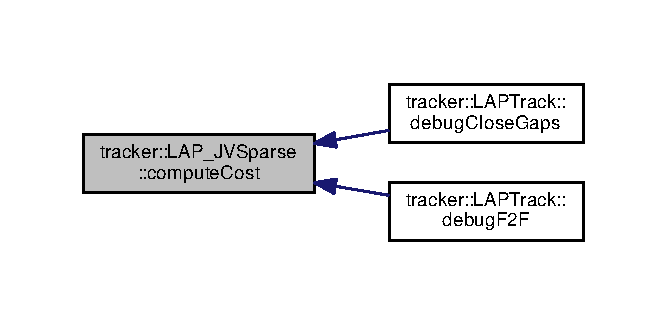
\includegraphics[width=320pt]{classtracker_1_1LAP__JVSparse_a4d731a155829c5f7c587afa0e518fe62_icgraph}
\end{center}
\end{figure}


\index{tracker\+::\+L\+A\+P\+\_\+\+J\+V\+Sparse@{tracker\+::\+L\+A\+P\+\_\+\+J\+V\+Sparse}!solve@{solve}}
\index{solve@{solve}!tracker\+::\+L\+A\+P\+\_\+\+J\+V\+Sparse@{tracker\+::\+L\+A\+P\+\_\+\+J\+V\+Sparse}}
\paragraph[{\texorpdfstring{solve(const Sp\+Mat\+T \&\+C)}{solve(const SpMatT &C)}}]{\setlength{\rightskip}{0pt plus 5cm}template$<$class FloatT $>$ {\bf L\+A\+P\+\_\+\+J\+V\+Sparse}$<$ FloatT $>$\+::I\+VecT {\bf tracker\+::\+L\+A\+P\+\_\+\+J\+V\+Sparse}$<$ FloatT $>$\+::solve (
\begin{DoxyParamCaption}
\item[{const Sp\+MatT \&}]{C}
\end{DoxyParamCaption}
)\hspace{0.3cm}{\ttfamily [static]}}\hypertarget{classtracker_1_1LAP__JVSparse_aea34e1276a8b6d217bd08a8a3b1156a8}{}\label{classtracker_1_1LAP__JVSparse_aea34e1276a8b6d217bd08a8a3b1156a8}


Definition at line 21 of file L\+A\+P\+\_\+\+J\+V\+Sparse.\+cpp.



Referenced by tracker\+::\+L\+A\+P\+Track\+::close\+Gaps(), tracker\+::\+L\+A\+P\+Track\+::debug\+Close\+Gaps(), tracker\+::\+L\+A\+P\+Track\+::debug\+F2\+F(), and tracker\+::\+L\+A\+P\+Track\+::link\+F2\+F().



Here is the caller graph for this function\+:\nopagebreak
\begin{figure}[H]
\begin{center}
\leavevmode
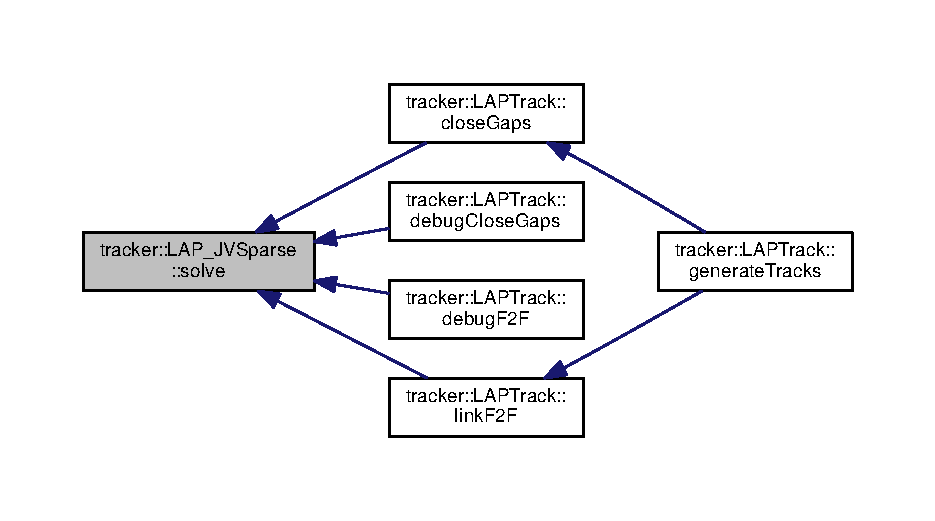
\includegraphics[width=350pt]{classtracker_1_1LAP__JVSparse_aea34e1276a8b6d217bd08a8a3b1156a8_icgraph}
\end{center}
\end{figure}


\index{tracker\+::\+L\+A\+P\+\_\+\+J\+V\+Sparse@{tracker\+::\+L\+A\+P\+\_\+\+J\+V\+Sparse}!solve\+L\+A\+P\+\_\+orig@{solve\+L\+A\+P\+\_\+orig}}
\index{solve\+L\+A\+P\+\_\+orig@{solve\+L\+A\+P\+\_\+orig}!tracker\+::\+L\+A\+P\+\_\+\+J\+V\+Sparse@{tracker\+::\+L\+A\+P\+\_\+\+J\+V\+Sparse}}
\paragraph[{\texorpdfstring{solve\+L\+A\+P\+\_\+orig(const Sp\+Mat\+T \&\+C, I\+Vec\+T \&x, I\+Vec\+T \&y, Vec\+T \&u, Vec\+T \&v)}{solveLAP_orig(const SpMatT &C, IVecT &x, IVecT &y, VecT &u, VecT &v)}}]{\setlength{\rightskip}{0pt plus 5cm}template$<$class FloatT $>$ void {\bf tracker\+::\+L\+A\+P\+\_\+\+J\+V\+Sparse}$<$ FloatT $>$\+::solve\+L\+A\+P\+\_\+orig (
\begin{DoxyParamCaption}
\item[{const Sp\+MatT \&}]{C, }
\item[{I\+VecT \&}]{x, }
\item[{I\+VecT \&}]{y, }
\item[{VecT \&}]{u, }
\item[{VecT \&}]{v}
\end{DoxyParamCaption}
)\hspace{0.3cm}{\ttfamily [static]}}\hypertarget{classtracker_1_1LAP__JVSparse_a2587babf5d28fee6c4e09659f492e58e}{}\label{classtracker_1_1LAP__JVSparse_a2587babf5d28fee6c4e09659f492e58e}
This wraps the original sparse lap implementation that for some reason uses 1-\/based indexing, which we correct with some pointer arrithmetic and adjusting of appropriate indicies in the sparse matrix implementation.

Furthermore because the lap\+\_\+orig code assumes a compressed-\/row format, but we pass it the internal datastore of a compressed-\/col format sparse metrix. We invert x/y and u/v on the call to lap\+\_\+orig to effectively let the transformation work easily with the legacy code.

This means x is the row sol and y is the col sol, as it normally would be.


\begin{DoxyParams}[1]{Parameters}
\mbox{\tt in}  & {\em C} & costs sparse matrix \\
\hline
\mbox{\tt out}  & {\em x} & -\/ row assignments \\
\hline
\mbox{\tt out}  & {\em y} & -\/ col assignments \\
\hline
\mbox{\tt out}  & {\em u} & -\/ reduced row costs \\
\hline
\mbox{\tt out}  & {\em v} & -\/ reduced column costs \\
\hline
\end{DoxyParams}


Definition at line 50 of file L\+A\+P\+\_\+\+J\+V\+Sparse.\+cpp.



The documentation for this class was generated from the following files\+:\begin{DoxyCompactItemize}
\item 
\hyperlink{LAP__JVSparse_8h}{L\+A\+P\+\_\+\+J\+V\+Sparse.\+h}\item 
\hyperlink{LAP__JVSparse_8cpp}{L\+A\+P\+\_\+\+J\+V\+Sparse.\+cpp}\end{DoxyCompactItemize}

\hypertarget{classtracker_1_1LAPTrack}{}\subsection{tracker\+:\+:L\+A\+P\+Track Class Reference}
\label{classtracker_1_1LAPTrack}\index{tracker\+::\+L\+A\+P\+Track@{tracker\+::\+L\+A\+P\+Track}}


{\ttfamily \#include $<$/home/travis/build/markjolah/\+Tracker/include/\+Tracker/\+L\+A\+P\+Track.\+h$>$}



Inheritance diagram for tracker\+:\+:L\+A\+P\+Track\+:\nopagebreak
\begin{figure}[H]
\begin{center}
\leavevmode
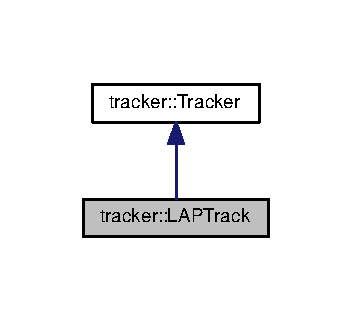
\includegraphics[width=169pt]{classtracker_1_1LAPTrack__inherit__graph}
\end{center}
\end{figure}


Collaboration diagram for tracker\+:\+:L\+A\+P\+Track\+:\nopagebreak
\begin{figure}[H]
\begin{center}
\leavevmode
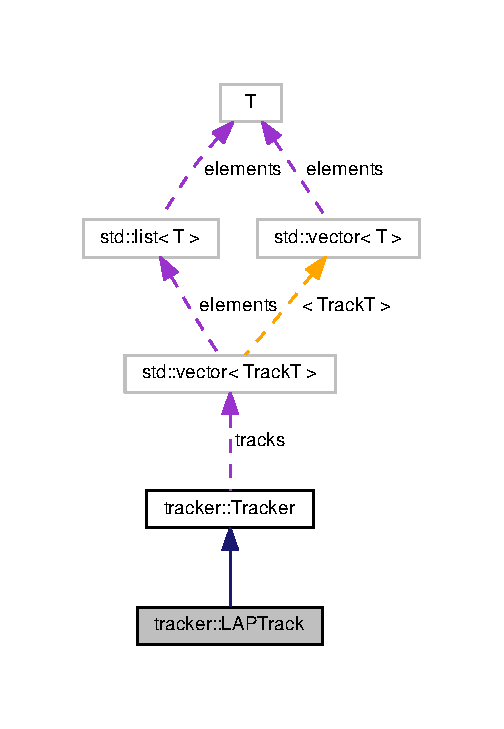
\includegraphics[width=242pt]{classtracker_1_1LAPTrack__coll__graph}
\end{center}
\end{figure}
\subsubsection*{Public Types}
\begin{DoxyCompactItemize}
\item 
using \hyperlink{classtracker_1_1LAPTrack_a85e4da204f0881dd4b46caf38bcef737}{Sp\+MatT} = arma\+::\+Sp\+Mat$<$ \hyperlink{classtracker_1_1Tracker_a66e8a81f12871e23082264c964f8f103}{FloatT} $>$
\item 
using \hyperlink{classtracker_1_1LAPTrack_aa2a2232f3db006d28422e54b9f236945}{U\+VecT} = arma\+::\+Col$<$ arma\+::uword $>$
\item 
using \hyperlink{classtracker_1_1LAPTrack_a24e342e3b28213ea690b9bb806fc380e}{U\+MatT} = arma\+::umat
\item 
using \hyperlink{classtracker_1_1Tracker_a66e8a81f12871e23082264c964f8f103}{FloatT} = double
\item 
using \hyperlink{classtracker_1_1Tracker_ad39a875dc6957cb6a9f3affcf6517d80}{IdxT} = int32\+\_\+t
\item 
using \hyperlink{classtracker_1_1Tracker_a9905fa9b81b252716e651d87d7d57aff}{VecT} = arma\+::\+Col$<$ \hyperlink{classtracker_1_1Tracker_a66e8a81f12871e23082264c964f8f103}{FloatT} $>$
\item 
using \hyperlink{classtracker_1_1Tracker_a60a1d6ee07284ba82f0533c79311ccfd}{MatT} = arma\+::\+Mat$<$ \hyperlink{classtracker_1_1Tracker_a66e8a81f12871e23082264c964f8f103}{FloatT} $>$
\item 
using \hyperlink{classtracker_1_1Tracker_a59a6e01be987f9c0093a8ac5ad97ce33}{I\+VecT} = arma\+::\+Col$<$ \hyperlink{classtracker_1_1Tracker_ad39a875dc6957cb6a9f3affcf6517d80}{IdxT} $>$
\item 
using \hyperlink{classtracker_1_1Tracker_a6de023cd3b5466996624c7e1b7e5d551}{I\+MatT} = arma\+::\+Mat$<$ \hyperlink{classtracker_1_1Tracker_ad39a875dc6957cb6a9f3affcf6517d80}{IdxT} $>$
\item 
using \hyperlink{classtracker_1_1Tracker_a122e1d351fcb4444aec9729cf7625322}{I\+Vec\+FieldT} = arma\+::field$<$ \hyperlink{classtracker_1_1Tracker_a59a6e01be987f9c0093a8ac5ad97ce33}{I\+VecT} $>$
\item 
using \hyperlink{classtracker_1_1Tracker_a50ae514521f940c08813b45f53b6ce2d}{Index\+VectorT} = std\+::vector$<$ \hyperlink{classtracker_1_1Tracker_ad39a875dc6957cb6a9f3affcf6517d80}{IdxT} $>$
\item 
using \hyperlink{classtracker_1_1Tracker_ac1b06aee1b9d85fb75cf6a9579eb0e84}{TrackT} = std\+::list$<$ \hyperlink{classtracker_1_1Tracker_ad39a875dc6957cb6a9f3affcf6517d80}{IdxT} $>$
\item 
using \hyperlink{classtracker_1_1Tracker_a25ee8479eb10f1619a8eefd5d310eeb7}{Track\+VecT} = std\+::vector$<$ \hyperlink{classtracker_1_1Tracker_ac1b06aee1b9d85fb75cf6a9579eb0e84}{TrackT} $>$
\item 
using \hyperlink{classtracker_1_1Tracker_a5fd443ec1139ed82910dd16316100db7}{ParamT} = std\+::map$<$ std\+::string, \hyperlink{classtracker_1_1Tracker_a66e8a81f12871e23082264c964f8f103}{FloatT} $>$
\item 
using \hyperlink{classtracker_1_1Tracker_a1a79f7073d8e1a032369dcc8105604ce}{Vec\+ParamT} = std\+::map$<$ std\+::string, \hyperlink{classtracker_1_1Tracker_a9905fa9b81b252716e651d87d7d57aff}{VecT} $>$
\end{DoxyCompactItemize}
\subsubsection*{Public Member Functions}
\begin{DoxyCompactItemize}
\item 
\hyperlink{classtracker_1_1LAPTrack_a276996ee58188944dd1d81f767ce0474}{L\+A\+P\+Track} (const \hyperlink{classtracker_1_1Tracker_a1a79f7073d8e1a032369dcc8105604ce}{Vec\+ParamT} \&param)
\item 
\hyperlink{classtracker_1_1Tracker_a1a79f7073d8e1a032369dcc8105604ce}{Vec\+ParamT} \hyperlink{classtracker_1_1LAPTrack_ab5dc7bdfbaafa9eafec4d9fd7ade3411}{get\+Stats} () const 
\item 
void \hyperlink{classtracker_1_1LAPTrack_a9561d939e76b3ed9afca03cc4d457c9e}{initialize\+Tracks} (const \hyperlink{classtracker_1_1Tracker_a59a6e01be987f9c0093a8ac5ad97ce33}{I\+VecT} \&frame\+Idx\+\_\+, const \hyperlink{classtracker_1_1Tracker_a60a1d6ee07284ba82f0533c79311ccfd}{MatT} \&position\+\_\+, const \hyperlink{classtracker_1_1Tracker_a60a1d6ee07284ba82f0533c79311ccfd}{MatT} \&S\+E\+\_\+position\+\_\+)
\item 
void \hyperlink{classtracker_1_1LAPTrack_a22ba01a68c707be9b3e906e14b84ff1f}{initialize\+Tracks} (const \hyperlink{classtracker_1_1Tracker_a59a6e01be987f9c0093a8ac5ad97ce33}{I\+VecT} \&frame\+Idx\+\_\+, const \hyperlink{classtracker_1_1Tracker_a60a1d6ee07284ba82f0533c79311ccfd}{MatT} \&position\+\_\+, const \hyperlink{classtracker_1_1Tracker_a60a1d6ee07284ba82f0533c79311ccfd}{MatT} \&S\+E\+\_\+position\+\_\+, const \hyperlink{classtracker_1_1Tracker_a60a1d6ee07284ba82f0533c79311ccfd}{MatT} \&feature\+\_\+, const \hyperlink{classtracker_1_1Tracker_a60a1d6ee07284ba82f0533c79311ccfd}{MatT} \&S\+E\+\_\+feature\+\_\+)
\item 
void \hyperlink{classtracker_1_1LAPTrack_acb3db52d2371baf8f96c35cf9e3741bd}{link\+F2F} ()
\item 
void \hyperlink{classtracker_1_1LAPTrack_a7e1ce573ac1f20bbb1f7bb6a51876525}{close\+Gaps} ()
\item 
\hyperlink{classtracker_1_1LAPTrack_a85e4da204f0881dd4b46caf38bcef737}{Sp\+MatT} \hyperlink{classtracker_1_1LAPTrack_a993c8f819a93d6d2ed442a1678c5ce81}{compute\+F2\+F\+Cost\+Mat} (int cur\+Frame, int next\+Frame) const 
\item 
void \hyperlink{classtracker_1_1LAPTrack_a1f334e86d674d5fa4eb69b281e3db62c}{debug\+F2F} (int \hyperlink{classtracker_1_1Tracker_aa3e32ff8183fe70af1d351f6324e7615}{frame\+Idx}, \hyperlink{classtracker_1_1Tracker_a59a6e01be987f9c0093a8ac5ad97ce33}{I\+VecT} \&cur\+\_\+locs, \hyperlink{classtracker_1_1Tracker_a59a6e01be987f9c0093a8ac5ad97ce33}{I\+VecT} \&next\+\_\+locs, \hyperlink{classtracker_1_1LAPTrack_a85e4da204f0881dd4b46caf38bcef737}{Sp\+MatT} \&cost, \hyperlink{classtracker_1_1Tracker_a6de023cd3b5466996624c7e1b7e5d551}{I\+MatT} \&connections, \hyperlink{classtracker_1_1Tracker_a9905fa9b81b252716e651d87d7d57aff}{VecT} \&conn\+\_\+costs) const 
\item 
void \hyperlink{classtracker_1_1LAPTrack_a52533a484c3fca552698a94785f5054a}{debug\+Close\+Gaps} (\hyperlink{classtracker_1_1LAPTrack_a85e4da204f0881dd4b46caf38bcef737}{Sp\+MatT} \&cost, \hyperlink{classtracker_1_1Tracker_a6de023cd3b5466996624c7e1b7e5d551}{I\+MatT} \&connections, \hyperlink{classtracker_1_1Tracker_a9905fa9b81b252716e651d87d7d57aff}{VecT} \&conn\+\_\+costs) const 
\item 
\hyperlink{classtracker_1_1LAPTrack_a85e4da204f0881dd4b46caf38bcef737}{Sp\+MatT} \hyperlink{classtracker_1_1LAPTrack_a3a195a7fa82a0019115bc3fd53a38e5f}{compute\+Gap\+Close\+Matrix} () const 
\item 
void \hyperlink{classtracker_1_1LAPTrack_aac61350c9f3e2c12c9aef7892a718f38}{generate\+Tracks} ()
\item 
void \hyperlink{classtracker_1_1LAPTrack_a0e7109c21c558f6ecd300f2a21416d4c}{check\+Frame\+Idxs} ()
\item 
void \hyperlink{classtracker_1_1Tracker_a5d1d2a969102d181b69b23333c874fc3}{print\+Tracks} () const 
\end{DoxyCompactItemize}
\subsubsection*{Public Attributes}
\begin{DoxyCompactItemize}
\item 
\hyperlink{classtracker_1_1Tracker_a66e8a81f12871e23082264c964f8f103}{FloatT} \hyperlink{classtracker_1_1LAPTrack_aeb0584b18f32b86e395de5a973108187}{D}
\item 
\hyperlink{classtracker_1_1Tracker_a66e8a81f12871e23082264c964f8f103}{FloatT} \hyperlink{classtracker_1_1LAPTrack_ad0e45f79d117cd5156818f27c3a41d45}{kon}
\item 
\hyperlink{classtracker_1_1Tracker_a66e8a81f12871e23082264c964f8f103}{FloatT} \hyperlink{classtracker_1_1LAPTrack_a726079bfbbc885c065086b76ee549bfa}{koff}
\item 
\hyperlink{classtracker_1_1Tracker_a66e8a81f12871e23082264c964f8f103}{FloatT} \hyperlink{classtracker_1_1LAPTrack_a67d4adb49fbda172c6ea701c93985713}{rho}
\item 
\hyperlink{classtracker_1_1Tracker_a9905fa9b81b252716e651d87d7d57aff}{VecT} \hyperlink{classtracker_1_1LAPTrack_a69599f06e61865ba634d6c88a1119319}{feature\+Var}
\item 
\hyperlink{classtracker_1_1Tracker_a66e8a81f12871e23082264c964f8f103}{FloatT} \hyperlink{classtracker_1_1LAPTrack_a8da459415ca2bb4f3d57b3c8db87e66e}{max\+Speed} = 0
\item 
\hyperlink{classtracker_1_1Tracker_a66e8a81f12871e23082264c964f8f103}{FloatT} \hyperlink{classtracker_1_1LAPTrack_ad3662aeeb356ae8dd4070f583a8ba9c9}{max\+Position\+Displacement\+Sigma} = 5.\+0
\item 
\hyperlink{classtracker_1_1Tracker_a9905fa9b81b252716e651d87d7d57aff}{VecT} \hyperlink{classtracker_1_1LAPTrack_a220f2d5a80b5999ed3c70e31a04901b0}{max\+Feature\+Displacement\+Sigma}
\item 
\hyperlink{classtracker_1_1Tracker_ad39a875dc6957cb6a9f3affcf6517d80}{IdxT} \hyperlink{classtracker_1_1LAPTrack_a3b70051e6eb22f9798c865109740ab48}{max\+Gap\+Close\+Frames} = 20
\item 
\hyperlink{classtracker_1_1Tracker_ad39a875dc6957cb6a9f3affcf6517d80}{IdxT} \hyperlink{classtracker_1_1LAPTrack_a580b1ec32d1e21c40e5a19f3f26518b4}{min\+Gap\+Close\+Track\+Length} = 1
\item 
\hyperlink{classtracker_1_1Tracker_ad39a875dc6957cb6a9f3affcf6517d80}{IdxT} \hyperlink{classtracker_1_1LAPTrack_a9a856327b91dddeb277b8a3633184cb3}{min\+Final\+Track\+Length} = 1
\item 
const \hyperlink{classtracker_1_1Tracker_a66e8a81f12871e23082264c964f8f103}{FloatT} \hyperlink{classtracker_1_1LAPTrack_a7e64b62f96af123e349ce5ba7801cced}{cost\+\_\+epsilon} = std\+::numeric\+\_\+limits$<$\hyperlink{classtracker_1_1Tracker_a66e8a81f12871e23082264c964f8f103}{FloatT}$>$\+::epsilon()
\item 
\hyperlink{classtracker_1_1Tracker_ad39a875dc6957cb6a9f3affcf6517d80}{IdxT} \hyperlink{classtracker_1_1Tracker_a5d8cb7831463035649c791311001228f}{N} = 0
\item 
\hyperlink{classtracker_1_1Tracker_ad39a875dc6957cb6a9f3affcf6517d80}{IdxT} \hyperlink{classtracker_1_1Tracker_a5efb17589760984816411fb6f69d561d}{n\+Dims} = 0
\item 
\hyperlink{classtracker_1_1Tracker_ad39a875dc6957cb6a9f3affcf6517d80}{IdxT} \hyperlink{classtracker_1_1Tracker_ade0b77f0b5ffc71aecddc70593ec16bb}{n\+Features} = 0
\item 
\hyperlink{classtracker_1_1Tracker_a59a6e01be987f9c0093a8ac5ad97ce33}{I\+VecT} \hyperlink{classtracker_1_1Tracker_aa3e32ff8183fe70af1d351f6324e7615}{frame\+Idx}
\item 
\hyperlink{classtracker_1_1Tracker_a60a1d6ee07284ba82f0533c79311ccfd}{MatT} \hyperlink{classtracker_1_1Tracker_a89978ed5ec72607820f45f3dcf63dd04}{position}
\item 
\hyperlink{classtracker_1_1Tracker_a60a1d6ee07284ba82f0533c79311ccfd}{MatT} \hyperlink{classtracker_1_1Tracker_acd4e8651a05dff9170230149b7fe0029}{S\+E\+\_\+position}
\item 
\hyperlink{classtracker_1_1Tracker_a60a1d6ee07284ba82f0533c79311ccfd}{MatT} \hyperlink{classtracker_1_1Tracker_ab9d6c09e4ae84ff482cd21cc32878138}{feature}
\item 
\hyperlink{classtracker_1_1Tracker_a60a1d6ee07284ba82f0533c79311ccfd}{MatT} \hyperlink{classtracker_1_1Tracker_a0aa2719b06bfd7b630628486b67ca5fd}{S\+E\+\_\+feature}
\item 
\hyperlink{classtracker_1_1Tracker_ad39a875dc6957cb6a9f3affcf6517d80}{IdxT} \hyperlink{classtracker_1_1Tracker_a3ba78a0a502bd2ac432601fc204e3ba1}{first\+Frame} = 0
\item 
\hyperlink{classtracker_1_1Tracker_ad39a875dc6957cb6a9f3affcf6517d80}{IdxT} \hyperlink{classtracker_1_1Tracker_af3219a1e02551ca5c6aafc4a8c14ff30}{last\+Frame} = 0
\item 
\hyperlink{classtracker_1_1Tracker_ad39a875dc6957cb6a9f3affcf6517d80}{IdxT} \hyperlink{classtracker_1_1Tracker_a103afa608ae5693103d81e040a9e29d6}{n\+Frames} = 0
\item 
\hyperlink{classtracker_1_1Tracker_a59a6e01be987f9c0093a8ac5ad97ce33}{I\+VecT} \hyperlink{classtracker_1_1Tracker_a84d3000b7a2b7a2566791f05d3b8afcb}{n\+Frame\+Locs}
\item 
\hyperlink{classtracker_1_1Tracker_a122e1d351fcb4444aec9729cf7625322}{I\+Vec\+FieldT} \hyperlink{classtracker_1_1Tracker_a089a3af55a168691f56d856658786159}{frame\+Loc\+Idx}
\item 
\hyperlink{classtracker_1_1Tracker_a25ee8479eb10f1619a8eefd5d310eeb7}{Track\+VecT} \hyperlink{classtracker_1_1Tracker_a1e43335eb50e56014399a157b261160b}{tracks}
\end{DoxyCompactItemize}
\subsubsection*{Protected Types}
\begin{DoxyCompactItemize}
\item 
enum \hyperlink{classtracker_1_1LAPTrack_ae474c311508c7e37bfd9080f3885f59b}{StateT} \{ \hyperlink{classtracker_1_1LAPTrack_ae474c311508c7e37bfd9080f3885f59ba0cb22a66c6ed4baeddea761814bb8bda}{U\+N\+T\+R\+A\+C\+K\+ED}, 
\hyperlink{classtracker_1_1LAPTrack_ae474c311508c7e37bfd9080f3885f59ba1f595bb9aff13fb50048ffda22ad8e73}{F2\+F\+\_\+\+L\+I\+N\+K\+ED}, 
\hyperlink{classtracker_1_1LAPTrack_ae474c311508c7e37bfd9080f3885f59bae1bc3dd81f059d3b28c1338111878699}{G\+A\+P\+S\+\_\+\+C\+L\+O\+S\+ED}
 \}
\end{DoxyCompactItemize}
\subsubsection*{Protected Attributes}
\begin{DoxyCompactItemize}
\item 
\hyperlink{classtracker_1_1Tracker_a66e8a81f12871e23082264c964f8f103}{FloatT} \hyperlink{classtracker_1_1LAPTrack_a6909c7f712dc8abbde326ef7c77d3885}{min\+Cost} = 1e-\/6
\item 
\hyperlink{classtracker_1_1Tracker_a66e8a81f12871e23082264c964f8f103}{FloatT} \hyperlink{classtracker_1_1LAPTrack_a0d698061ef3117aed73b71975b217ef1}{log1mkoff}
\item 
\hyperlink{classtracker_1_1Tracker_a66e8a81f12871e23082264c964f8f103}{FloatT} \hyperlink{classtracker_1_1LAPTrack_ac0e506d8b8b4e29689cbf2a112f86df4}{log1mkon}
\item 
\hyperlink{classtracker_1_1Tracker_a66e8a81f12871e23082264c964f8f103}{FloatT} \hyperlink{classtracker_1_1LAPTrack_a95e4746d8eac4e665e0bb34be5ad4198}{logrho}
\item 
\hyperlink{classtracker_1_1Tracker_a66e8a81f12871e23082264c964f8f103}{FloatT} \hyperlink{classtracker_1_1LAPTrack_ac257b647714df10faf5c3bc15ae9ed43}{logkon}
\item 
\hyperlink{classtracker_1_1Tracker_a66e8a81f12871e23082264c964f8f103}{FloatT} \hyperlink{classtracker_1_1LAPTrack_a75af05f0cad86fd46bcb32ac63e36abb}{logkoff}
\item 
\hyperlink{classtracker_1_1LAPTrack_ae474c311508c7e37bfd9080f3885f59b}{StateT} \hyperlink{classtracker_1_1LAPTrack_a0e74c48780822951efdc3570348a3dd5}{state}
\item 
\hyperlink{classtracker_1_1Tracker_a50ae514521f940c08813b45f53b6ce2d}{Index\+VectorT} \hyperlink{classtracker_1_1LAPTrack_a56dd0c2e669f3311471a817d2c12595c}{birth\+Frame\+Idx}
\item 
\hyperlink{classtracker_1_1Tracker_a59a6e01be987f9c0093a8ac5ad97ce33}{I\+VecT} \hyperlink{classtracker_1_1LAPTrack_a19b9e3e8cc4e908fa2e3816f386a7f27}{frame\+Birth\+Start\+Idx}
\item 
\hyperlink{classtracker_1_1Tracker_a59a6e01be987f9c0093a8ac5ad97ce33}{I\+VecT} \hyperlink{classtracker_1_1Tracker_a638ecbd5a6466c2730e7c7b9561e9fc9}{track\+Assignment}
\end{DoxyCompactItemize}
\subsubsection*{Static Protected Attributes}
\begin{DoxyCompactItemize}
\item 
static const \hyperlink{classtracker_1_1Tracker_a66e8a81f12871e23082264c964f8f103}{FloatT} \hyperlink{classtracker_1_1Tracker_adf40b4f798f070419f5eb697b36b65ac}{log2pi} = log(2$\ast$arma\+::\+Datum$<$\hyperlink{classtracker_1_1Tracker_a66e8a81f12871e23082264c964f8f103}{Tracker\+::\+FloatT}$>$\+::pi)
\end{DoxyCompactItemize}


\subsubsection{Detailed Description}


Definition at line 16 of file L\+A\+P\+Track.\+h.



\subsubsection{Member Typedef Documentation}
\index{tracker\+::\+L\+A\+P\+Track@{tracker\+::\+L\+A\+P\+Track}!FloatT@{FloatT}}
\index{FloatT@{FloatT}!tracker\+::\+L\+A\+P\+Track@{tracker\+::\+L\+A\+P\+Track}}
\paragraph[{\texorpdfstring{FloatT}{FloatT}}]{\setlength{\rightskip}{0pt plus 5cm}using {\bf tracker\+::\+Tracker\+::\+FloatT} =  double\hspace{0.3cm}{\ttfamily [inherited]}}\hypertarget{classtracker_1_1Tracker_a66e8a81f12871e23082264c964f8f103}{}\label{classtracker_1_1Tracker_a66e8a81f12871e23082264c964f8f103}


Definition at line 47 of file Tracker.\+h.

\index{tracker\+::\+L\+A\+P\+Track@{tracker\+::\+L\+A\+P\+Track}!IdxT@{IdxT}}
\index{IdxT@{IdxT}!tracker\+::\+L\+A\+P\+Track@{tracker\+::\+L\+A\+P\+Track}}
\paragraph[{\texorpdfstring{IdxT}{IdxT}}]{\setlength{\rightskip}{0pt plus 5cm}using {\bf tracker\+::\+Tracker\+::\+IdxT} =  int32\+\_\+t\hspace{0.3cm}{\ttfamily [inherited]}}\hypertarget{classtracker_1_1Tracker_ad39a875dc6957cb6a9f3affcf6517d80}{}\label{classtracker_1_1Tracker_ad39a875dc6957cb6a9f3affcf6517d80}


Definition at line 48 of file Tracker.\+h.

\index{tracker\+::\+L\+A\+P\+Track@{tracker\+::\+L\+A\+P\+Track}!I\+MatT@{I\+MatT}}
\index{I\+MatT@{I\+MatT}!tracker\+::\+L\+A\+P\+Track@{tracker\+::\+L\+A\+P\+Track}}
\paragraph[{\texorpdfstring{I\+MatT}{IMatT}}]{\setlength{\rightskip}{0pt plus 5cm}using {\bf tracker\+::\+Tracker\+::\+I\+MatT} =  arma\+::\+Mat$<${\bf IdxT}$>$\hspace{0.3cm}{\ttfamily [inherited]}}\hypertarget{classtracker_1_1Tracker_a6de023cd3b5466996624c7e1b7e5d551}{}\label{classtracker_1_1Tracker_a6de023cd3b5466996624c7e1b7e5d551}


Definition at line 52 of file Tracker.\+h.

\index{tracker\+::\+L\+A\+P\+Track@{tracker\+::\+L\+A\+P\+Track}!Index\+VectorT@{Index\+VectorT}}
\index{Index\+VectorT@{Index\+VectorT}!tracker\+::\+L\+A\+P\+Track@{tracker\+::\+L\+A\+P\+Track}}
\paragraph[{\texorpdfstring{Index\+VectorT}{IndexVectorT}}]{\setlength{\rightskip}{0pt plus 5cm}using {\bf tracker\+::\+Tracker\+::\+Index\+VectorT} =  std\+::vector$<${\bf IdxT}$>$\hspace{0.3cm}{\ttfamily [inherited]}}\hypertarget{classtracker_1_1Tracker_a50ae514521f940c08813b45f53b6ce2d}{}\label{classtracker_1_1Tracker_a50ae514521f940c08813b45f53b6ce2d}


Definition at line 54 of file Tracker.\+h.

\index{tracker\+::\+L\+A\+P\+Track@{tracker\+::\+L\+A\+P\+Track}!I\+Vec\+FieldT@{I\+Vec\+FieldT}}
\index{I\+Vec\+FieldT@{I\+Vec\+FieldT}!tracker\+::\+L\+A\+P\+Track@{tracker\+::\+L\+A\+P\+Track}}
\paragraph[{\texorpdfstring{I\+Vec\+FieldT}{IVecFieldT}}]{\setlength{\rightskip}{0pt plus 5cm}using {\bf tracker\+::\+Tracker\+::\+I\+Vec\+FieldT} =  arma\+::field$<${\bf I\+VecT}$>$\hspace{0.3cm}{\ttfamily [inherited]}}\hypertarget{classtracker_1_1Tracker_a122e1d351fcb4444aec9729cf7625322}{}\label{classtracker_1_1Tracker_a122e1d351fcb4444aec9729cf7625322}


Definition at line 53 of file Tracker.\+h.

\index{tracker\+::\+L\+A\+P\+Track@{tracker\+::\+L\+A\+P\+Track}!I\+VecT@{I\+VecT}}
\index{I\+VecT@{I\+VecT}!tracker\+::\+L\+A\+P\+Track@{tracker\+::\+L\+A\+P\+Track}}
\paragraph[{\texorpdfstring{I\+VecT}{IVecT}}]{\setlength{\rightskip}{0pt plus 5cm}using {\bf tracker\+::\+Tracker\+::\+I\+VecT} =  arma\+::\+Col$<${\bf IdxT}$>$\hspace{0.3cm}{\ttfamily [inherited]}}\hypertarget{classtracker_1_1Tracker_a59a6e01be987f9c0093a8ac5ad97ce33}{}\label{classtracker_1_1Tracker_a59a6e01be987f9c0093a8ac5ad97ce33}


Definition at line 51 of file Tracker.\+h.

\index{tracker\+::\+L\+A\+P\+Track@{tracker\+::\+L\+A\+P\+Track}!MatT@{MatT}}
\index{MatT@{MatT}!tracker\+::\+L\+A\+P\+Track@{tracker\+::\+L\+A\+P\+Track}}
\paragraph[{\texorpdfstring{MatT}{MatT}}]{\setlength{\rightskip}{0pt plus 5cm}using {\bf tracker\+::\+Tracker\+::\+MatT} =  arma\+::\+Mat$<${\bf FloatT}$>$\hspace{0.3cm}{\ttfamily [inherited]}}\hypertarget{classtracker_1_1Tracker_a60a1d6ee07284ba82f0533c79311ccfd}{}\label{classtracker_1_1Tracker_a60a1d6ee07284ba82f0533c79311ccfd}


Definition at line 50 of file Tracker.\+h.

\index{tracker\+::\+L\+A\+P\+Track@{tracker\+::\+L\+A\+P\+Track}!ParamT@{ParamT}}
\index{ParamT@{ParamT}!tracker\+::\+L\+A\+P\+Track@{tracker\+::\+L\+A\+P\+Track}}
\paragraph[{\texorpdfstring{ParamT}{ParamT}}]{\setlength{\rightskip}{0pt plus 5cm}using {\bf tracker\+::\+Tracker\+::\+ParamT} =  std\+::map$<$std\+::string,{\bf FloatT}$>$\hspace{0.3cm}{\ttfamily [inherited]}}\hypertarget{classtracker_1_1Tracker_a5fd443ec1139ed82910dd16316100db7}{}\label{classtracker_1_1Tracker_a5fd443ec1139ed82910dd16316100db7}
A convenient form for reporting dictionaries of named FP data to matlab 

Definition at line 57 of file Tracker.\+h.

\index{tracker\+::\+L\+A\+P\+Track@{tracker\+::\+L\+A\+P\+Track}!Sp\+MatT@{Sp\+MatT}}
\index{Sp\+MatT@{Sp\+MatT}!tracker\+::\+L\+A\+P\+Track@{tracker\+::\+L\+A\+P\+Track}}
\paragraph[{\texorpdfstring{Sp\+MatT}{SpMatT}}]{\setlength{\rightskip}{0pt plus 5cm}using {\bf tracker\+::\+L\+A\+P\+Track\+::\+Sp\+MatT} =  arma\+::\+Sp\+Mat$<${\bf FloatT}$>$}\hypertarget{classtracker_1_1LAPTrack_a85e4da204f0881dd4b46caf38bcef737}{}\label{classtracker_1_1LAPTrack_a85e4da204f0881dd4b46caf38bcef737}


Definition at line 18 of file L\+A\+P\+Track.\+h.

\index{tracker\+::\+L\+A\+P\+Track@{tracker\+::\+L\+A\+P\+Track}!TrackT@{TrackT}}
\index{TrackT@{TrackT}!tracker\+::\+L\+A\+P\+Track@{tracker\+::\+L\+A\+P\+Track}}
\paragraph[{\texorpdfstring{TrackT}{TrackT}}]{\setlength{\rightskip}{0pt plus 5cm}using {\bf tracker\+::\+Tracker\+::\+TrackT} =  std\+::list$<${\bf IdxT}$>$\hspace{0.3cm}{\ttfamily [inherited]}}\hypertarget{classtracker_1_1Tracker_ac1b06aee1b9d85fb75cf6a9579eb0e84}{}\label{classtracker_1_1Tracker_ac1b06aee1b9d85fb75cf6a9579eb0e84}
A type for an individual track 

Definition at line 55 of file Tracker.\+h.

\index{tracker\+::\+L\+A\+P\+Track@{tracker\+::\+L\+A\+P\+Track}!Track\+VecT@{Track\+VecT}}
\index{Track\+VecT@{Track\+VecT}!tracker\+::\+L\+A\+P\+Track@{tracker\+::\+L\+A\+P\+Track}}
\paragraph[{\texorpdfstring{Track\+VecT}{TrackVecT}}]{\setlength{\rightskip}{0pt plus 5cm}using {\bf tracker\+::\+Tracker\+::\+Track\+VecT} =  std\+::vector$<${\bf TrackT}$>$\hspace{0.3cm}{\ttfamily [inherited]}}\hypertarget{classtracker_1_1Tracker_a25ee8479eb10f1619a8eefd5d310eeb7}{}\label{classtracker_1_1Tracker_a25ee8479eb10f1619a8eefd5d310eeb7}
A type for a vector of tracks 

Definition at line 56 of file Tracker.\+h.

\index{tracker\+::\+L\+A\+P\+Track@{tracker\+::\+L\+A\+P\+Track}!U\+MatT@{U\+MatT}}
\index{U\+MatT@{U\+MatT}!tracker\+::\+L\+A\+P\+Track@{tracker\+::\+L\+A\+P\+Track}}
\paragraph[{\texorpdfstring{U\+MatT}{UMatT}}]{\setlength{\rightskip}{0pt plus 5cm}using {\bf tracker\+::\+L\+A\+P\+Track\+::\+U\+MatT} =  arma\+::umat}\hypertarget{classtracker_1_1LAPTrack_a24e342e3b28213ea690b9bb806fc380e}{}\label{classtracker_1_1LAPTrack_a24e342e3b28213ea690b9bb806fc380e}


Definition at line 20 of file L\+A\+P\+Track.\+h.

\index{tracker\+::\+L\+A\+P\+Track@{tracker\+::\+L\+A\+P\+Track}!U\+VecT@{U\+VecT}}
\index{U\+VecT@{U\+VecT}!tracker\+::\+L\+A\+P\+Track@{tracker\+::\+L\+A\+P\+Track}}
\paragraph[{\texorpdfstring{U\+VecT}{UVecT}}]{\setlength{\rightskip}{0pt plus 5cm}using {\bf tracker\+::\+L\+A\+P\+Track\+::\+U\+VecT} =  arma\+::\+Col$<$arma\+::uword$>$}\hypertarget{classtracker_1_1LAPTrack_aa2a2232f3db006d28422e54b9f236945}{}\label{classtracker_1_1LAPTrack_aa2a2232f3db006d28422e54b9f236945}


Definition at line 19 of file L\+A\+P\+Track.\+h.

\index{tracker\+::\+L\+A\+P\+Track@{tracker\+::\+L\+A\+P\+Track}!Vec\+ParamT@{Vec\+ParamT}}
\index{Vec\+ParamT@{Vec\+ParamT}!tracker\+::\+L\+A\+P\+Track@{tracker\+::\+L\+A\+P\+Track}}
\paragraph[{\texorpdfstring{Vec\+ParamT}{VecParamT}}]{\setlength{\rightskip}{0pt plus 5cm}using {\bf tracker\+::\+Tracker\+::\+Vec\+ParamT} =  std\+::map$<$std\+::string,{\bf VecT}$>$\hspace{0.3cm}{\ttfamily [inherited]}}\hypertarget{classtracker_1_1Tracker_a1a79f7073d8e1a032369dcc8105604ce}{}\label{classtracker_1_1Tracker_a1a79f7073d8e1a032369dcc8105604ce}
A convenient form for reporting dictionaries of named FP data to matlab 

Definition at line 58 of file Tracker.\+h.

\index{tracker\+::\+L\+A\+P\+Track@{tracker\+::\+L\+A\+P\+Track}!VecT@{VecT}}
\index{VecT@{VecT}!tracker\+::\+L\+A\+P\+Track@{tracker\+::\+L\+A\+P\+Track}}
\paragraph[{\texorpdfstring{VecT}{VecT}}]{\setlength{\rightskip}{0pt plus 5cm}using {\bf tracker\+::\+Tracker\+::\+VecT} =  arma\+::\+Col$<${\bf FloatT}$>$\hspace{0.3cm}{\ttfamily [inherited]}}\hypertarget{classtracker_1_1Tracker_a9905fa9b81b252716e651d87d7d57aff}{}\label{classtracker_1_1Tracker_a9905fa9b81b252716e651d87d7d57aff}


Definition at line 49 of file Tracker.\+h.



\subsubsection{Member Enumeration Documentation}
\index{tracker\+::\+L\+A\+P\+Track@{tracker\+::\+L\+A\+P\+Track}!StateT@{StateT}}
\index{StateT@{StateT}!tracker\+::\+L\+A\+P\+Track@{tracker\+::\+L\+A\+P\+Track}}
\paragraph[{\texorpdfstring{StateT}{StateT}}]{\setlength{\rightskip}{0pt plus 5cm}enum {\bf tracker\+::\+L\+A\+P\+Track\+::\+StateT}\hspace{0.3cm}{\ttfamily [protected]}}\hypertarget{classtracker_1_1LAPTrack_ae474c311508c7e37bfd9080f3885f59b}{}\label{classtracker_1_1LAPTrack_ae474c311508c7e37bfd9080f3885f59b}
\begin{Desc}
\item[Enumerator]\par
\begin{description}
\index{U\+N\+T\+R\+A\+C\+K\+ED@{U\+N\+T\+R\+A\+C\+K\+ED}!tracker\+::\+L\+A\+P\+Track@{tracker\+::\+L\+A\+P\+Track}}\index{tracker\+::\+L\+A\+P\+Track@{tracker\+::\+L\+A\+P\+Track}!U\+N\+T\+R\+A\+C\+K\+ED@{U\+N\+T\+R\+A\+C\+K\+ED}}\item[{\em 
U\+N\+T\+R\+A\+C\+K\+ED\hypertarget{classtracker_1_1LAPTrack_ae474c311508c7e37bfd9080f3885f59ba0cb22a66c6ed4baeddea761814bb8bda}{}\label{classtracker_1_1LAPTrack_ae474c311508c7e37bfd9080f3885f59ba0cb22a66c6ed4baeddea761814bb8bda}
}]\index{F2\+F\+\_\+\+L\+I\+N\+K\+ED@{F2\+F\+\_\+\+L\+I\+N\+K\+ED}!tracker\+::\+L\+A\+P\+Track@{tracker\+::\+L\+A\+P\+Track}}\index{tracker\+::\+L\+A\+P\+Track@{tracker\+::\+L\+A\+P\+Track}!F2\+F\+\_\+\+L\+I\+N\+K\+ED@{F2\+F\+\_\+\+L\+I\+N\+K\+ED}}\item[{\em 
F2\+F\+\_\+\+L\+I\+N\+K\+ED\hypertarget{classtracker_1_1LAPTrack_ae474c311508c7e37bfd9080f3885f59ba1f595bb9aff13fb50048ffda22ad8e73}{}\label{classtracker_1_1LAPTrack_ae474c311508c7e37bfd9080f3885f59ba1f595bb9aff13fb50048ffda22ad8e73}
}]\index{G\+A\+P\+S\+\_\+\+C\+L\+O\+S\+ED@{G\+A\+P\+S\+\_\+\+C\+L\+O\+S\+ED}!tracker\+::\+L\+A\+P\+Track@{tracker\+::\+L\+A\+P\+Track}}\index{tracker\+::\+L\+A\+P\+Track@{tracker\+::\+L\+A\+P\+Track}!G\+A\+P\+S\+\_\+\+C\+L\+O\+S\+ED@{G\+A\+P\+S\+\_\+\+C\+L\+O\+S\+ED}}\item[{\em 
G\+A\+P\+S\+\_\+\+C\+L\+O\+S\+ED\hypertarget{classtracker_1_1LAPTrack_ae474c311508c7e37bfd9080f3885f59bae1bc3dd81f059d3b28c1338111878699}{}\label{classtracker_1_1LAPTrack_ae474c311508c7e37bfd9080f3885f59bae1bc3dd81f059d3b28c1338111878699}
}]\end{description}
\end{Desc}


Definition at line 58 of file L\+A\+P\+Track.\+h.



\subsubsection{Constructor \& Destructor Documentation}
\index{tracker\+::\+L\+A\+P\+Track@{tracker\+::\+L\+A\+P\+Track}!L\+A\+P\+Track@{L\+A\+P\+Track}}
\index{L\+A\+P\+Track@{L\+A\+P\+Track}!tracker\+::\+L\+A\+P\+Track@{tracker\+::\+L\+A\+P\+Track}}
\paragraph[{\texorpdfstring{L\+A\+P\+Track(const Vec\+Param\+T \&param)}{LAPTrack(const VecParamT &param)}}]{\setlength{\rightskip}{0pt plus 5cm}tracker\+::\+L\+A\+P\+Track\+::\+L\+A\+P\+Track (
\begin{DoxyParamCaption}
\item[{const {\bf Vec\+ParamT} \&}]{param}
\end{DoxyParamCaption}
)}\hypertarget{classtracker_1_1LAPTrack_a276996ee58188944dd1d81f767ce0474}{}\label{classtracker_1_1LAPTrack_a276996ee58188944dd1d81f767ce0474}


Definition at line 11 of file L\+A\+P\+Track.\+cpp.



References D, feature\+Var, koff, kon, log1mkoff, log1mkon, logkoff, logkon, logrho, max\+Feature\+Displacement\+Sigma, max\+Gap\+Close\+Frames, max\+Position\+Displacement\+Sigma, max\+Speed, min\+Final\+Track\+Length, min\+Gap\+Close\+Track\+Length, and rho.



\subsubsection{Member Function Documentation}
\index{tracker\+::\+L\+A\+P\+Track@{tracker\+::\+L\+A\+P\+Track}!check\+Frame\+Idxs@{check\+Frame\+Idxs}}
\index{check\+Frame\+Idxs@{check\+Frame\+Idxs}!tracker\+::\+L\+A\+P\+Track@{tracker\+::\+L\+A\+P\+Track}}
\paragraph[{\texorpdfstring{check\+Frame\+Idxs()}{checkFrameIdxs()}}]{\setlength{\rightskip}{0pt plus 5cm}void tracker\+::\+L\+A\+P\+Track\+::check\+Frame\+Idxs (
\begin{DoxyParamCaption}
{}
\end{DoxyParamCaption}
)}\hypertarget{classtracker_1_1LAPTrack_a0e7109c21c558f6ecd300f2a21416d4c}{}\label{classtracker_1_1LAPTrack_a0e7109c21c558f6ecd300f2a21416d4c}


Definition at line 335 of file L\+A\+P\+Track.\+cpp.



References F2\+F\+\_\+\+L\+I\+N\+K\+ED, tracker\+::\+Tracker\+::first\+Frame, frame\+Birth\+Start\+Idx, tracker\+::\+Tracker\+::frame\+Idx, tracker\+::\+Tracker\+::last\+Frame, state, and tracker\+::\+Tracker\+::tracks.

\index{tracker\+::\+L\+A\+P\+Track@{tracker\+::\+L\+A\+P\+Track}!close\+Gaps@{close\+Gaps}}
\index{close\+Gaps@{close\+Gaps}!tracker\+::\+L\+A\+P\+Track@{tracker\+::\+L\+A\+P\+Track}}
\paragraph[{\texorpdfstring{close\+Gaps()}{closeGaps()}}]{\setlength{\rightskip}{0pt plus 5cm}void tracker\+::\+L\+A\+P\+Track\+::close\+Gaps (
\begin{DoxyParamCaption}
{}
\end{DoxyParamCaption}
)}\hypertarget{classtracker_1_1LAPTrack_a7e1ce573ac1f20bbb1f7bb6a51876525}{}\label{classtracker_1_1LAPTrack_a7e1ce573ac1f20bbb1f7bb6a51876525}


Definition at line 376 of file L\+A\+P\+Track.\+cpp.



References birth\+Frame\+Idx, compute\+Gap\+Close\+Matrix(), F2\+F\+\_\+\+L\+I\+N\+K\+ED, frame\+Birth\+Start\+Idx, G\+A\+P\+S\+\_\+\+C\+L\+O\+S\+ED, min\+Final\+Track\+Length, tracker\+::\+L\+A\+P\+\_\+\+J\+V\+Sparse$<$ Float\+T $>$\+::solve(), state, tracker\+::\+Tracker\+::track\+Assignment, and tracker\+::\+Tracker\+::tracks.



Referenced by generate\+Tracks().



Here is the call graph for this function\+:\nopagebreak
\begin{figure}[H]
\begin{center}
\leavevmode
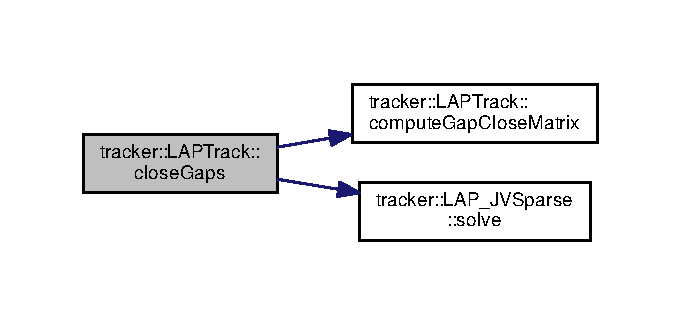
\includegraphics[width=327pt]{classtracker_1_1LAPTrack_a7e1ce573ac1f20bbb1f7bb6a51876525_cgraph}
\end{center}
\end{figure}




Here is the caller graph for this function\+:\nopagebreak
\begin{figure}[H]
\begin{center}
\leavevmode
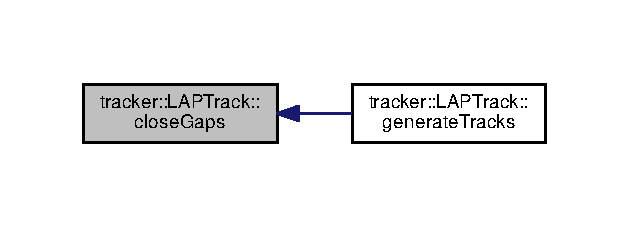
\includegraphics[width=302pt]{classtracker_1_1LAPTrack_a7e1ce573ac1f20bbb1f7bb6a51876525_icgraph}
\end{center}
\end{figure}


\index{tracker\+::\+L\+A\+P\+Track@{tracker\+::\+L\+A\+P\+Track}!compute\+F2\+F\+Cost\+Mat@{compute\+F2\+F\+Cost\+Mat}}
\index{compute\+F2\+F\+Cost\+Mat@{compute\+F2\+F\+Cost\+Mat}!tracker\+::\+L\+A\+P\+Track@{tracker\+::\+L\+A\+P\+Track}}
\paragraph[{\texorpdfstring{compute\+F2\+F\+Cost\+Mat(int cur\+Frame, int next\+Frame) const }{computeF2FCostMat(int curFrame, int nextFrame) const }}]{\setlength{\rightskip}{0pt plus 5cm}{\bf L\+A\+P\+Track\+::\+Sp\+MatT} tracker\+::\+L\+A\+P\+Track\+::compute\+F2\+F\+Cost\+Mat (
\begin{DoxyParamCaption}
\item[{int}]{cur\+Frame, }
\item[{int}]{next\+Frame}
\end{DoxyParamCaption}
) const}\hypertarget{classtracker_1_1LAPTrack_a993c8f819a93d6d2ed442a1678c5ce81}{}\label{classtracker_1_1LAPTrack_a993c8f819a93d6d2ed442a1678c5ce81}


Definition at line 231 of file L\+A\+P\+Track.\+cpp.



References cost\+\_\+epsilon, D, tracker\+::\+Tracker\+::feature, feature\+Var, tracker\+::\+Tracker\+::first\+Frame, tracker\+::\+Tracker\+::frame\+Loc\+Idx, log1mkoff, tracker\+::\+Tracker\+::log2pi, logkoff, logkon, logrho, max\+Feature\+Displacement\+Sigma, max\+Position\+Displacement\+Sigma, max\+Speed, tracker\+::\+Tracker\+::n\+Dims, tracker\+::\+Tracker\+::n\+Features, tracker\+::\+Tracker\+::n\+Frame\+Locs, tracker\+::\+Tracker\+::position, tracker\+::\+Tracker\+::\+S\+E\+\_\+feature, and tracker\+::\+Tracker\+::\+S\+E\+\_\+position.



Referenced by debug\+F2\+F(), and link\+F2\+F().



Here is the caller graph for this function\+:\nopagebreak
\begin{figure}[H]
\begin{center}
\leavevmode
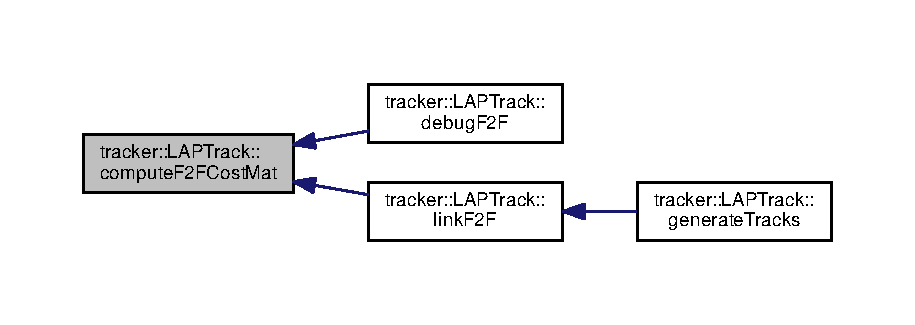
\includegraphics[width=350pt]{classtracker_1_1LAPTrack_a993c8f819a93d6d2ed442a1678c5ce81_icgraph}
\end{center}
\end{figure}


\index{tracker\+::\+L\+A\+P\+Track@{tracker\+::\+L\+A\+P\+Track}!compute\+Gap\+Close\+Matrix@{compute\+Gap\+Close\+Matrix}}
\index{compute\+Gap\+Close\+Matrix@{compute\+Gap\+Close\+Matrix}!tracker\+::\+L\+A\+P\+Track@{tracker\+::\+L\+A\+P\+Track}}
\paragraph[{\texorpdfstring{compute\+Gap\+Close\+Matrix() const }{computeGapCloseMatrix() const }}]{\setlength{\rightskip}{0pt plus 5cm}{\bf L\+A\+P\+Track\+::\+Sp\+MatT} tracker\+::\+L\+A\+P\+Track\+::compute\+Gap\+Close\+Matrix (
\begin{DoxyParamCaption}
{}
\end{DoxyParamCaption}
) const}\hypertarget{classtracker_1_1LAPTrack_a3a195a7fa82a0019115bc3fd53a38e5f}{}\label{classtracker_1_1LAPTrack_a3a195a7fa82a0019115bc3fd53a38e5f}


Definition at line 415 of file L\+A\+P\+Track.\+cpp.



References birth\+Frame\+Idx, cost\+\_\+epsilon, D, tracker\+::\+Tracker\+::feature, feature\+Var, tracker\+::\+Tracker\+::first\+Frame, frame\+Birth\+Start\+Idx, tracker\+::\+Tracker\+::frame\+Idx, tracker\+::\+Tracker\+::last\+Frame, tracker\+::\+Tracker\+::log2pi, logkoff, logkon, logrho, max\+Feature\+Displacement\+Sigma, max\+Gap\+Close\+Frames, max\+Position\+Displacement\+Sigma, max\+Speed, min\+Gap\+Close\+Track\+Length, tracker\+::\+Tracker\+::n\+Dims, tracker\+::\+Tracker\+::n\+Features, tracker\+::\+Tracker\+::position, tracker\+::\+Tracker\+::\+S\+E\+\_\+feature, tracker\+::\+Tracker\+::\+S\+E\+\_\+position, and tracker\+::\+Tracker\+::tracks.



Referenced by close\+Gaps(), and debug\+Close\+Gaps().



Here is the caller graph for this function\+:\nopagebreak
\begin{figure}[H]
\begin{center}
\leavevmode
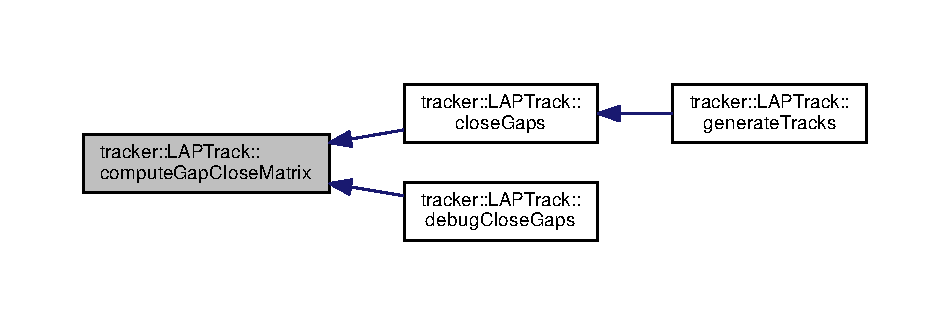
\includegraphics[width=350pt]{classtracker_1_1LAPTrack_a3a195a7fa82a0019115bc3fd53a38e5f_icgraph}
\end{center}
\end{figure}


\index{tracker\+::\+L\+A\+P\+Track@{tracker\+::\+L\+A\+P\+Track}!debug\+Close\+Gaps@{debug\+Close\+Gaps}}
\index{debug\+Close\+Gaps@{debug\+Close\+Gaps}!tracker\+::\+L\+A\+P\+Track@{tracker\+::\+L\+A\+P\+Track}}
\paragraph[{\texorpdfstring{debug\+Close\+Gaps(\+Sp\+Mat\+T \&cost, I\+Mat\+T \&connections, Vec\+T \&conn\+\_\+costs) const }{debugCloseGaps(SpMatT &cost, IMatT &connections, VecT &conn_costs) const }}]{\setlength{\rightskip}{0pt plus 5cm}void tracker\+::\+L\+A\+P\+Track\+::debug\+Close\+Gaps (
\begin{DoxyParamCaption}
\item[{{\bf Sp\+MatT} \&}]{cost, }
\item[{{\bf I\+MatT} \&}]{connections, }
\item[{{\bf VecT} \&}]{conn\+\_\+costs}
\end{DoxyParamCaption}
) const}\hypertarget{classtracker_1_1LAPTrack_a52533a484c3fca552698a94785f5054a}{}\label{classtracker_1_1LAPTrack_a52533a484c3fca552698a94785f5054a}


Definition at line 351 of file L\+A\+P\+Track.\+cpp.



References tracker\+::\+L\+A\+P\+\_\+\+J\+V\+Sparse$<$ Float\+T $>$\+::compute\+Cost(), compute\+Gap\+Close\+Matrix(), cost\+\_\+epsilon, F2\+F\+\_\+\+L\+I\+N\+K\+ED, tracker\+::\+L\+A\+P\+\_\+\+J\+V\+Sparse$<$ Float\+T $>$\+::solve(), state, and tracker\+::\+Tracker\+::tracks.



Here is the call graph for this function\+:\nopagebreak
\begin{figure}[H]
\begin{center}
\leavevmode
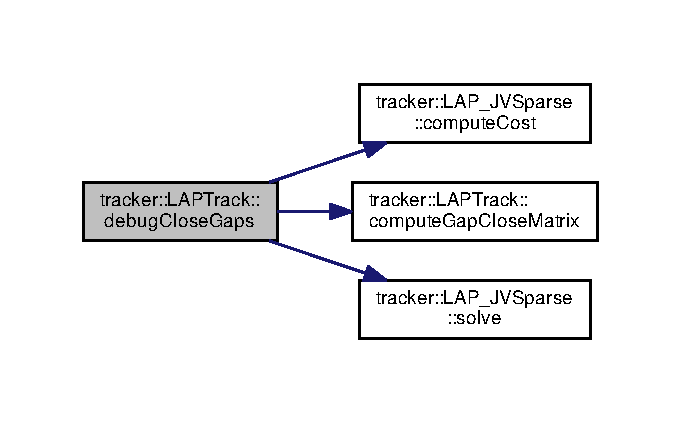
\includegraphics[width=327pt]{classtracker_1_1LAPTrack_a52533a484c3fca552698a94785f5054a_cgraph}
\end{center}
\end{figure}


\index{tracker\+::\+L\+A\+P\+Track@{tracker\+::\+L\+A\+P\+Track}!debug\+F2F@{debug\+F2F}}
\index{debug\+F2F@{debug\+F2F}!tracker\+::\+L\+A\+P\+Track@{tracker\+::\+L\+A\+P\+Track}}
\paragraph[{\texorpdfstring{debug\+F2\+F(int frame\+Idx, I\+Vec\+T \&cur\+\_\+locs, I\+Vec\+T \&next\+\_\+locs, Sp\+Mat\+T \&cost, I\+Mat\+T \&connections, Vec\+T \&conn\+\_\+costs) const }{debugF2F(int frameIdx, IVecT &cur_locs, IVecT &next_locs, SpMatT &cost, IMatT &connections, VecT &conn_costs) const }}]{\setlength{\rightskip}{0pt plus 5cm}void tracker\+::\+L\+A\+P\+Track\+::debug\+F2F (
\begin{DoxyParamCaption}
\item[{int}]{frame\+Idx, }
\item[{{\bf I\+VecT} \&}]{cur\+\_\+locs, }
\item[{{\bf I\+VecT} \&}]{next\+\_\+locs, }
\item[{{\bf Sp\+MatT} \&}]{cost, }
\item[{{\bf I\+MatT} \&}]{connections, }
\item[{{\bf VecT} \&}]{conn\+\_\+costs}
\end{DoxyParamCaption}
) const}\hypertarget{classtracker_1_1LAPTrack_a1f334e86d674d5fa4eb69b281e3db62c}{}\label{classtracker_1_1LAPTrack_a1f334e86d674d5fa4eb69b281e3db62c}


Definition at line 92 of file L\+A\+P\+Track.\+cpp.



References tracker\+::\+L\+A\+P\+\_\+\+J\+V\+Sparse$<$ Float\+T $>$\+::compute\+Cost(), compute\+F2\+F\+Cost\+Mat(), cost\+\_\+epsilon, tracker\+::\+Tracker\+::first\+Frame, tracker\+::\+Tracker\+::frame\+Loc\+Idx, tracker\+::\+Tracker\+::last\+Frame, tracker\+::\+Tracker\+::n\+Frame\+Locs, and tracker\+::\+L\+A\+P\+\_\+\+J\+V\+Sparse$<$ Float\+T $>$\+::solve().



Here is the call graph for this function\+:\nopagebreak
\begin{figure}[H]
\begin{center}
\leavevmode
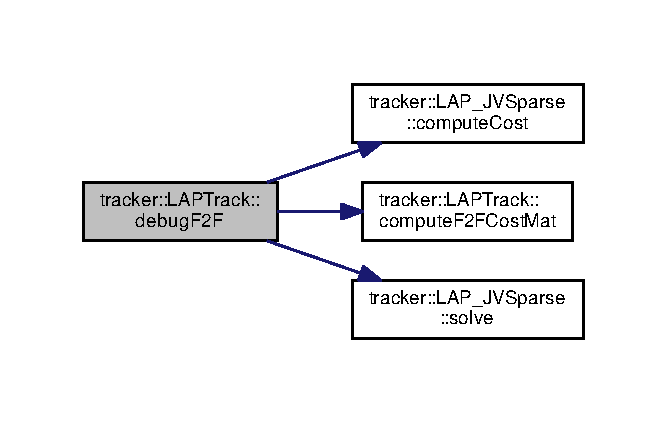
\includegraphics[width=320pt]{classtracker_1_1LAPTrack_a1f334e86d674d5fa4eb69b281e3db62c_cgraph}
\end{center}
\end{figure}


\index{tracker\+::\+L\+A\+P\+Track@{tracker\+::\+L\+A\+P\+Track}!generate\+Tracks@{generate\+Tracks}}
\index{generate\+Tracks@{generate\+Tracks}!tracker\+::\+L\+A\+P\+Track@{tracker\+::\+L\+A\+P\+Track}}
\paragraph[{\texorpdfstring{generate\+Tracks()}{generateTracks()}}]{\setlength{\rightskip}{0pt plus 5cm}void tracker\+::\+L\+A\+P\+Track\+::generate\+Tracks (
\begin{DoxyParamCaption}
{}
\end{DoxyParamCaption}
)\hspace{0.3cm}{\ttfamily [virtual]}}\hypertarget{classtracker_1_1LAPTrack_aac61350c9f3e2c12c9aef7892a718f38}{}\label{classtracker_1_1LAPTrack_aac61350c9f3e2c12c9aef7892a718f38}


Implements \hyperlink{classtracker_1_1Tracker_a14823a45c80086192c92aa90eb58ca17}{tracker\+::\+Tracker}.



Definition at line 77 of file L\+A\+P\+Track.\+cpp.



References close\+Gaps(), F2\+F\+\_\+\+L\+I\+N\+K\+ED, G\+A\+P\+S\+\_\+\+C\+L\+O\+S\+ED, link\+F2\+F(), state, and U\+N\+T\+R\+A\+C\+K\+ED.



Here is the call graph for this function\+:\nopagebreak
\begin{figure}[H]
\begin{center}
\leavevmode
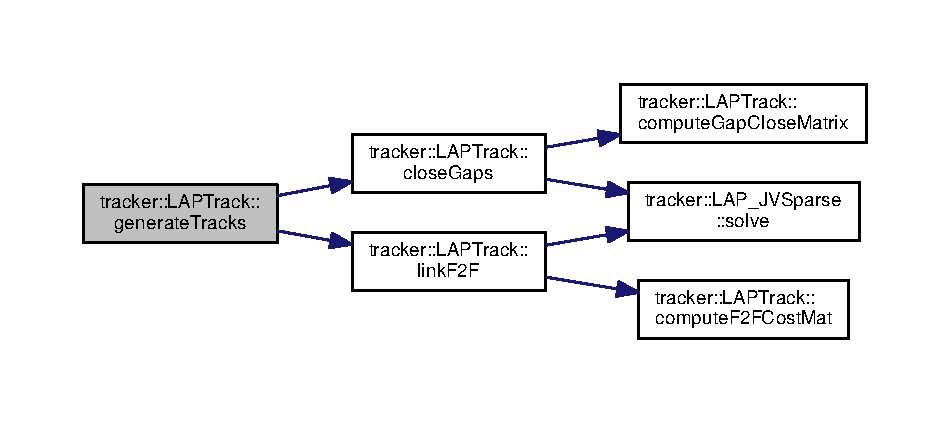
\includegraphics[width=350pt]{classtracker_1_1LAPTrack_aac61350c9f3e2c12c9aef7892a718f38_cgraph}
\end{center}
\end{figure}


\index{tracker\+::\+L\+A\+P\+Track@{tracker\+::\+L\+A\+P\+Track}!get\+Stats@{get\+Stats}}
\index{get\+Stats@{get\+Stats}!tracker\+::\+L\+A\+P\+Track@{tracker\+::\+L\+A\+P\+Track}}
\paragraph[{\texorpdfstring{get\+Stats() const }{getStats() const }}]{\setlength{\rightskip}{0pt plus 5cm}{\bf L\+A\+P\+Track\+::\+Vec\+ParamT} tracker\+::\+L\+A\+P\+Track\+::get\+Stats (
\begin{DoxyParamCaption}
{}
\end{DoxyParamCaption}
) const\hspace{0.3cm}{\ttfamily [virtual]}}\hypertarget{classtracker_1_1LAPTrack_ab5dc7bdfbaafa9eafec4d9fd7ade3411}{}\label{classtracker_1_1LAPTrack_ab5dc7bdfbaafa9eafec4d9fd7ade3411}


Reimplemented from \hyperlink{classtracker_1_1Tracker_a0ff525214ca14a98bacb8af427000cfa}{tracker\+::\+Tracker}.



Definition at line 46 of file L\+A\+P\+Track.\+cpp.



References D, feature\+Var, tracker\+::\+Tracker\+::get\+Stats(), koff, kon, max\+Feature\+Displacement\+Sigma, max\+Gap\+Close\+Frames, max\+Position\+Displacement\+Sigma, max\+Speed, min\+Final\+Track\+Length, min\+Gap\+Close\+Track\+Length, and rho.



Here is the call graph for this function\+:\nopagebreak
\begin{figure}[H]
\begin{center}
\leavevmode
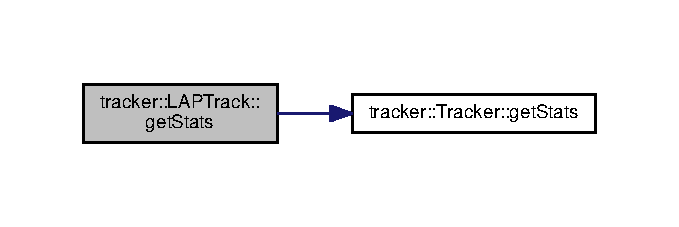
\includegraphics[width=326pt]{classtracker_1_1LAPTrack_ab5dc7bdfbaafa9eafec4d9fd7ade3411_cgraph}
\end{center}
\end{figure}


\index{tracker\+::\+L\+A\+P\+Track@{tracker\+::\+L\+A\+P\+Track}!initialize\+Tracks@{initialize\+Tracks}}
\index{initialize\+Tracks@{initialize\+Tracks}!tracker\+::\+L\+A\+P\+Track@{tracker\+::\+L\+A\+P\+Track}}
\paragraph[{\texorpdfstring{initialize\+Tracks(const I\+Vec\+T \&frame\+Idx\+\_\+, const Mat\+T \&position\+\_\+, const Mat\+T \&\+S\+E\+\_\+position\+\_\+)}{initializeTracks(const IVecT &frameIdx_, const MatT &position_, const MatT &SE_position_)}}]{\setlength{\rightskip}{0pt plus 5cm}void tracker\+::\+L\+A\+P\+Track\+::initialize\+Tracks (
\begin{DoxyParamCaption}
\item[{const {\bf I\+VecT} \&}]{frame\+Idx\+\_\+, }
\item[{const {\bf MatT} \&}]{position\+\_\+, }
\item[{const {\bf MatT} \&}]{S\+E\+\_\+position\+\_\+}
\end{DoxyParamCaption}
)\hspace{0.3cm}{\ttfamily [virtual]}}\hypertarget{classtracker_1_1LAPTrack_a9561d939e76b3ed9afca03cc4d457c9e}{}\label{classtracker_1_1LAPTrack_a9561d939e76b3ed9afca03cc4d457c9e}


Reimplemented from \hyperlink{classtracker_1_1Tracker_a54cebc540275536380aca0d9ecb7e575}{tracker\+::\+Tracker}.



Definition at line 63 of file L\+A\+P\+Track.\+cpp.

\index{tracker\+::\+L\+A\+P\+Track@{tracker\+::\+L\+A\+P\+Track}!initialize\+Tracks@{initialize\+Tracks}}
\index{initialize\+Tracks@{initialize\+Tracks}!tracker\+::\+L\+A\+P\+Track@{tracker\+::\+L\+A\+P\+Track}}
\paragraph[{\texorpdfstring{initialize\+Tracks(const I\+Vec\+T \&frame\+Idx\+\_\+, const Mat\+T \&position\+\_\+, const Mat\+T \&\+S\+E\+\_\+position\+\_\+, const Mat\+T \&feature\+\_\+, const Mat\+T \&\+S\+E\+\_\+feature\+\_\+)}{initializeTracks(const IVecT &frameIdx_, const MatT &position_, const MatT &SE_position_, const MatT &feature_, const MatT &SE_feature_)}}]{\setlength{\rightskip}{0pt plus 5cm}void tracker\+::\+L\+A\+P\+Track\+::initialize\+Tracks (
\begin{DoxyParamCaption}
\item[{const {\bf I\+VecT} \&}]{frame\+Idx\+\_\+, }
\item[{const {\bf MatT} \&}]{position\+\_\+, }
\item[{const {\bf MatT} \&}]{S\+E\+\_\+position\+\_\+, }
\item[{const {\bf MatT} \&}]{feature\+\_\+, }
\item[{const {\bf MatT} \&}]{S\+E\+\_\+feature\+\_\+}
\end{DoxyParamCaption}
)\hspace{0.3cm}{\ttfamily [virtual]}}\hypertarget{classtracker_1_1LAPTrack_a22ba01a68c707be9b3e906e14b84ff1f}{}\label{classtracker_1_1LAPTrack_a22ba01a68c707be9b3e906e14b84ff1f}


Reimplemented from \hyperlink{classtracker_1_1Tracker_a9fbf44fc368d294b47cd3bc48c0c69bd}{tracker\+::\+Tracker}.



Definition at line 69 of file L\+A\+P\+Track.\+cpp.



References birth\+Frame\+Idx, frame\+Birth\+Start\+Idx, tracker\+::\+Tracker\+::initialize\+Tracks(), state, and U\+N\+T\+R\+A\+C\+K\+ED.



Here is the call graph for this function\+:\nopagebreak
\begin{figure}[H]
\begin{center}
\leavevmode
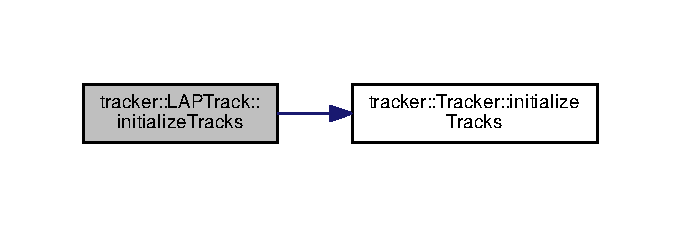
\includegraphics[width=327pt]{classtracker_1_1LAPTrack_a22ba01a68c707be9b3e906e14b84ff1f_cgraph}
\end{center}
\end{figure}


\index{tracker\+::\+L\+A\+P\+Track@{tracker\+::\+L\+A\+P\+Track}!link\+F2F@{link\+F2F}}
\index{link\+F2F@{link\+F2F}!tracker\+::\+L\+A\+P\+Track@{tracker\+::\+L\+A\+P\+Track}}
\paragraph[{\texorpdfstring{link\+F2\+F()}{linkF2F()}}]{\setlength{\rightskip}{0pt plus 5cm}void tracker\+::\+L\+A\+P\+Track\+::link\+F2F (
\begin{DoxyParamCaption}
{}
\end{DoxyParamCaption}
)}\hypertarget{classtracker_1_1LAPTrack_acb3db52d2371baf8f96c35cf9e3741bd}{}\label{classtracker_1_1LAPTrack_acb3db52d2371baf8f96c35cf9e3741bd}


Definition at line 130 of file L\+A\+P\+Track.\+cpp.



References birth\+Frame\+Idx, compute\+F2\+F\+Cost\+Mat(), F2\+F\+\_\+\+L\+I\+N\+K\+ED, tracker\+::\+Tracker\+::first\+Frame, frame\+Birth\+Start\+Idx, tracker\+::\+Tracker\+::frame\+Loc\+Idx, tracker\+::\+Tracker\+::last\+Frame, tracker\+::\+Tracker\+::n\+Frame\+Locs, tracker\+::\+Tracker\+::n\+Frames, tracker\+::\+L\+A\+P\+\_\+\+J\+V\+Sparse$<$ Float\+T $>$\+::solve(), state, tracker\+::\+Tracker\+::track\+Assignment, tracker\+::\+Tracker\+::tracks, and U\+N\+T\+R\+A\+C\+K\+ED.



Referenced by generate\+Tracks().



Here is the call graph for this function\+:\nopagebreak
\begin{figure}[H]
\begin{center}
\leavevmode
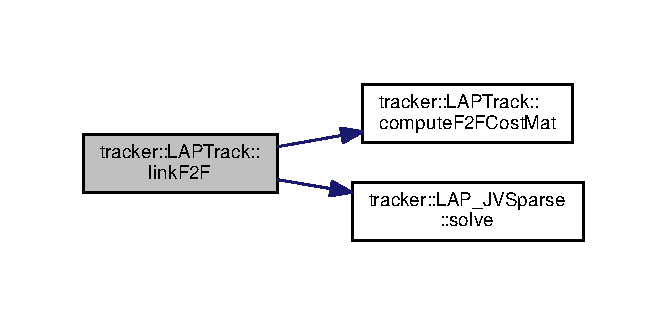
\includegraphics[width=320pt]{classtracker_1_1LAPTrack_acb3db52d2371baf8f96c35cf9e3741bd_cgraph}
\end{center}
\end{figure}




Here is the caller graph for this function\+:\nopagebreak
\begin{figure}[H]
\begin{center}
\leavevmode
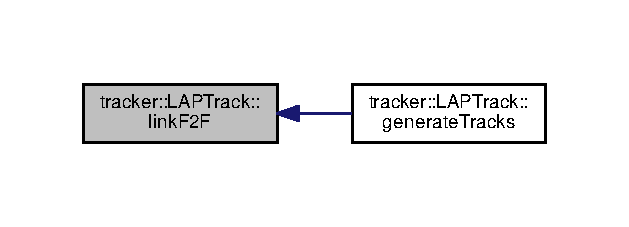
\includegraphics[width=302pt]{classtracker_1_1LAPTrack_acb3db52d2371baf8f96c35cf9e3741bd_icgraph}
\end{center}
\end{figure}


\index{tracker\+::\+L\+A\+P\+Track@{tracker\+::\+L\+A\+P\+Track}!print\+Tracks@{print\+Tracks}}
\index{print\+Tracks@{print\+Tracks}!tracker\+::\+L\+A\+P\+Track@{tracker\+::\+L\+A\+P\+Track}}
\paragraph[{\texorpdfstring{print\+Tracks() const }{printTracks() const }}]{\setlength{\rightskip}{0pt plus 5cm}void tracker\+::\+Tracker\+::print\+Tracks (
\begin{DoxyParamCaption}
{}
\end{DoxyParamCaption}
) const\hspace{0.3cm}{\ttfamily [inherited]}}\hypertarget{classtracker_1_1Tracker_a5d1d2a969102d181b69b23333c874fc3}{}\label{classtracker_1_1Tracker_a5d1d2a969102d181b69b23333c874fc3}


Definition at line 126 of file Tracker.\+cpp.



References tracker\+::\+Tracker\+::frame\+Idx, and tracker\+::\+Tracker\+::tracks.



\subsubsection{Member Data Documentation}
\index{tracker\+::\+L\+A\+P\+Track@{tracker\+::\+L\+A\+P\+Track}!birth\+Frame\+Idx@{birth\+Frame\+Idx}}
\index{birth\+Frame\+Idx@{birth\+Frame\+Idx}!tracker\+::\+L\+A\+P\+Track@{tracker\+::\+L\+A\+P\+Track}}
\paragraph[{\texorpdfstring{birth\+Frame\+Idx}{birthFrameIdx}}]{\setlength{\rightskip}{0pt plus 5cm}{\bf Index\+VectorT} tracker\+::\+L\+A\+P\+Track\+::birth\+Frame\+Idx\hspace{0.3cm}{\ttfamily [protected]}}\hypertarget{classtracker_1_1LAPTrack_a56dd0c2e669f3311471a817d2c12595c}{}\label{classtracker_1_1LAPTrack_a56dd0c2e669f3311471a817d2c12595c}


Definition at line 62 of file L\+A\+P\+Track.\+h.



Referenced by close\+Gaps(), compute\+Gap\+Close\+Matrix(), initialize\+Tracks(), and link\+F2\+F().

\index{tracker\+::\+L\+A\+P\+Track@{tracker\+::\+L\+A\+P\+Track}!cost\+\_\+epsilon@{cost\+\_\+epsilon}}
\index{cost\+\_\+epsilon@{cost\+\_\+epsilon}!tracker\+::\+L\+A\+P\+Track@{tracker\+::\+L\+A\+P\+Track}}
\paragraph[{\texorpdfstring{cost\+\_\+epsilon}{cost_epsilon}}]{\setlength{\rightskip}{0pt plus 5cm}const {\bf FloatT} tracker\+::\+L\+A\+P\+Track\+::cost\+\_\+epsilon = std\+::numeric\+\_\+limits$<${\bf FloatT}$>$\+::epsilon()}\hypertarget{classtracker_1_1LAPTrack_a7e64b62f96af123e349ce5ba7801cced}{}\label{classtracker_1_1LAPTrack_a7e64b62f96af123e349ce5ba7801cced}


Definition at line 35 of file L\+A\+P\+Track.\+h.



Referenced by compute\+F2\+F\+Cost\+Mat(), compute\+Gap\+Close\+Matrix(), debug\+Close\+Gaps(), and debug\+F2\+F().

\index{tracker\+::\+L\+A\+P\+Track@{tracker\+::\+L\+A\+P\+Track}!D@{D}}
\index{D@{D}!tracker\+::\+L\+A\+P\+Track@{tracker\+::\+L\+A\+P\+Track}}
\paragraph[{\texorpdfstring{D}{D}}]{\setlength{\rightskip}{0pt plus 5cm}{\bf FloatT} tracker\+::\+L\+A\+P\+Track\+::D}\hypertarget{classtracker_1_1LAPTrack_aeb0584b18f32b86e395de5a973108187}{}\label{classtracker_1_1LAPTrack_aeb0584b18f32b86e395de5a973108187}


Definition at line 22 of file L\+A\+P\+Track.\+h.



Referenced by compute\+F2\+F\+Cost\+Mat(), compute\+Gap\+Close\+Matrix(), get\+Stats(), and L\+A\+P\+Track().

\index{tracker\+::\+L\+A\+P\+Track@{tracker\+::\+L\+A\+P\+Track}!feature@{feature}}
\index{feature@{feature}!tracker\+::\+L\+A\+P\+Track@{tracker\+::\+L\+A\+P\+Track}}
\paragraph[{\texorpdfstring{feature}{feature}}]{\setlength{\rightskip}{0pt plus 5cm}{\bf MatT} tracker\+::\+Tracker\+::feature\hspace{0.3cm}{\ttfamily [inherited]}}\hypertarget{classtracker_1_1Tracker_ab9d6c09e4ae84ff482cd21cc32878138}{}\label{classtracker_1_1Tracker_ab9d6c09e4ae84ff482cd21cc32878138}


Definition at line 66 of file Tracker.\+h.



Referenced by compute\+F2\+F\+Cost\+Mat(), compute\+Gap\+Close\+Matrix(), and tracker\+::\+Tracker\+::initialize\+Tracks().

\index{tracker\+::\+L\+A\+P\+Track@{tracker\+::\+L\+A\+P\+Track}!feature\+Var@{feature\+Var}}
\index{feature\+Var@{feature\+Var}!tracker\+::\+L\+A\+P\+Track@{tracker\+::\+L\+A\+P\+Track}}
\paragraph[{\texorpdfstring{feature\+Var}{featureVar}}]{\setlength{\rightskip}{0pt plus 5cm}{\bf VecT} tracker\+::\+L\+A\+P\+Track\+::feature\+Var}\hypertarget{classtracker_1_1LAPTrack_a69599f06e61865ba634d6c88a1119319}{}\label{classtracker_1_1LAPTrack_a69599f06e61865ba634d6c88a1119319}


Definition at line 26 of file L\+A\+P\+Track.\+h.



Referenced by compute\+F2\+F\+Cost\+Mat(), compute\+Gap\+Close\+Matrix(), get\+Stats(), and L\+A\+P\+Track().

\index{tracker\+::\+L\+A\+P\+Track@{tracker\+::\+L\+A\+P\+Track}!first\+Frame@{first\+Frame}}
\index{first\+Frame@{first\+Frame}!tracker\+::\+L\+A\+P\+Track@{tracker\+::\+L\+A\+P\+Track}}
\paragraph[{\texorpdfstring{first\+Frame}{firstFrame}}]{\setlength{\rightskip}{0pt plus 5cm}{\bf IdxT} tracker\+::\+Tracker\+::first\+Frame = 0\hspace{0.3cm}{\ttfamily [inherited]}}\hypertarget{classtracker_1_1Tracker_a3ba78a0a502bd2ac432601fc204e3ba1}{}\label{classtracker_1_1Tracker_a3ba78a0a502bd2ac432601fc204e3ba1}


Definition at line 68 of file Tracker.\+h.



Referenced by check\+Frame\+Idxs(), compute\+F2\+F\+Cost\+Mat(), compute\+Gap\+Close\+Matrix(), debug\+F2\+F(), tracker\+::\+Tracker\+::get\+Stats(), tracker\+::\+Tracker\+::initialize\+Tracks(), and link\+F2\+F().

\index{tracker\+::\+L\+A\+P\+Track@{tracker\+::\+L\+A\+P\+Track}!frame\+Birth\+Start\+Idx@{frame\+Birth\+Start\+Idx}}
\index{frame\+Birth\+Start\+Idx@{frame\+Birth\+Start\+Idx}!tracker\+::\+L\+A\+P\+Track@{tracker\+::\+L\+A\+P\+Track}}
\paragraph[{\texorpdfstring{frame\+Birth\+Start\+Idx}{frameBirthStartIdx}}]{\setlength{\rightskip}{0pt plus 5cm}{\bf I\+VecT} tracker\+::\+L\+A\+P\+Track\+::frame\+Birth\+Start\+Idx\hspace{0.3cm}{\ttfamily [protected]}}\hypertarget{classtracker_1_1LAPTrack_a19b9e3e8cc4e908fa2e3816f386a7f27}{}\label{classtracker_1_1LAPTrack_a19b9e3e8cc4e908fa2e3816f386a7f27}


Definition at line 63 of file L\+A\+P\+Track.\+h.



Referenced by check\+Frame\+Idxs(), close\+Gaps(), compute\+Gap\+Close\+Matrix(), initialize\+Tracks(), and link\+F2\+F().

\index{tracker\+::\+L\+A\+P\+Track@{tracker\+::\+L\+A\+P\+Track}!frame\+Idx@{frame\+Idx}}
\index{frame\+Idx@{frame\+Idx}!tracker\+::\+L\+A\+P\+Track@{tracker\+::\+L\+A\+P\+Track}}
\paragraph[{\texorpdfstring{frame\+Idx}{frameIdx}}]{\setlength{\rightskip}{0pt plus 5cm}{\bf I\+VecT} tracker\+::\+Tracker\+::frame\+Idx\hspace{0.3cm}{\ttfamily [inherited]}}\hypertarget{classtracker_1_1Tracker_aa3e32ff8183fe70af1d351f6324e7615}{}\label{classtracker_1_1Tracker_aa3e32ff8183fe70af1d351f6324e7615}


Definition at line 63 of file Tracker.\+h.



Referenced by check\+Frame\+Idxs(), compute\+Gap\+Close\+Matrix(), tracker\+::\+Tracker\+::initialize\+Tracks(), and tracker\+::\+Tracker\+::print\+Tracks().

\index{tracker\+::\+L\+A\+P\+Track@{tracker\+::\+L\+A\+P\+Track}!frame\+Loc\+Idx@{frame\+Loc\+Idx}}
\index{frame\+Loc\+Idx@{frame\+Loc\+Idx}!tracker\+::\+L\+A\+P\+Track@{tracker\+::\+L\+A\+P\+Track}}
\paragraph[{\texorpdfstring{frame\+Loc\+Idx}{frameLocIdx}}]{\setlength{\rightskip}{0pt plus 5cm}{\bf I\+Vec\+FieldT} tracker\+::\+Tracker\+::frame\+Loc\+Idx\hspace{0.3cm}{\ttfamily [inherited]}}\hypertarget{classtracker_1_1Tracker_a089a3af55a168691f56d856658786159}{}\label{classtracker_1_1Tracker_a089a3af55a168691f56d856658786159}


Definition at line 74 of file Tracker.\+h.



Referenced by compute\+F2\+F\+Cost\+Mat(), debug\+F2\+F(), tracker\+::\+Tracker\+::initialize\+Tracks(), and link\+F2\+F().

\index{tracker\+::\+L\+A\+P\+Track@{tracker\+::\+L\+A\+P\+Track}!koff@{koff}}
\index{koff@{koff}!tracker\+::\+L\+A\+P\+Track@{tracker\+::\+L\+A\+P\+Track}}
\paragraph[{\texorpdfstring{koff}{koff}}]{\setlength{\rightskip}{0pt plus 5cm}{\bf FloatT} tracker\+::\+L\+A\+P\+Track\+::koff}\hypertarget{classtracker_1_1LAPTrack_a726079bfbbc885c065086b76ee549bfa}{}\label{classtracker_1_1LAPTrack_a726079bfbbc885c065086b76ee549bfa}


Definition at line 24 of file L\+A\+P\+Track.\+h.



Referenced by get\+Stats(), and L\+A\+P\+Track().

\index{tracker\+::\+L\+A\+P\+Track@{tracker\+::\+L\+A\+P\+Track}!kon@{kon}}
\index{kon@{kon}!tracker\+::\+L\+A\+P\+Track@{tracker\+::\+L\+A\+P\+Track}}
\paragraph[{\texorpdfstring{kon}{kon}}]{\setlength{\rightskip}{0pt plus 5cm}{\bf FloatT} tracker\+::\+L\+A\+P\+Track\+::kon}\hypertarget{classtracker_1_1LAPTrack_ad0e45f79d117cd5156818f27c3a41d45}{}\label{classtracker_1_1LAPTrack_ad0e45f79d117cd5156818f27c3a41d45}


Definition at line 23 of file L\+A\+P\+Track.\+h.



Referenced by get\+Stats(), and L\+A\+P\+Track().

\index{tracker\+::\+L\+A\+P\+Track@{tracker\+::\+L\+A\+P\+Track}!last\+Frame@{last\+Frame}}
\index{last\+Frame@{last\+Frame}!tracker\+::\+L\+A\+P\+Track@{tracker\+::\+L\+A\+P\+Track}}
\paragraph[{\texorpdfstring{last\+Frame}{lastFrame}}]{\setlength{\rightskip}{0pt plus 5cm}{\bf IdxT} tracker\+::\+Tracker\+::last\+Frame = 0\hspace{0.3cm}{\ttfamily [inherited]}}\hypertarget{classtracker_1_1Tracker_af3219a1e02551ca5c6aafc4a8c14ff30}{}\label{classtracker_1_1Tracker_af3219a1e02551ca5c6aafc4a8c14ff30}


Definition at line 69 of file Tracker.\+h.



Referenced by check\+Frame\+Idxs(), compute\+Gap\+Close\+Matrix(), debug\+F2\+F(), tracker\+::\+Tracker\+::get\+Stats(), tracker\+::\+Tracker\+::initialize\+Tracks(), and link\+F2\+F().

\index{tracker\+::\+L\+A\+P\+Track@{tracker\+::\+L\+A\+P\+Track}!log1mkoff@{log1mkoff}}
\index{log1mkoff@{log1mkoff}!tracker\+::\+L\+A\+P\+Track@{tracker\+::\+L\+A\+P\+Track}}
\paragraph[{\texorpdfstring{log1mkoff}{log1mkoff}}]{\setlength{\rightskip}{0pt plus 5cm}{\bf FloatT} tracker\+::\+L\+A\+P\+Track\+::log1mkoff\hspace{0.3cm}{\ttfamily [protected]}}\hypertarget{classtracker_1_1LAPTrack_a0d698061ef3117aed73b71975b217ef1}{}\label{classtracker_1_1LAPTrack_a0d698061ef3117aed73b71975b217ef1}


Definition at line 52 of file L\+A\+P\+Track.\+h.



Referenced by compute\+F2\+F\+Cost\+Mat(), and L\+A\+P\+Track().

\index{tracker\+::\+L\+A\+P\+Track@{tracker\+::\+L\+A\+P\+Track}!log1mkon@{log1mkon}}
\index{log1mkon@{log1mkon}!tracker\+::\+L\+A\+P\+Track@{tracker\+::\+L\+A\+P\+Track}}
\paragraph[{\texorpdfstring{log1mkon}{log1mkon}}]{\setlength{\rightskip}{0pt plus 5cm}{\bf FloatT} tracker\+::\+L\+A\+P\+Track\+::log1mkon\hspace{0.3cm}{\ttfamily [protected]}}\hypertarget{classtracker_1_1LAPTrack_ac0e506d8b8b4e29689cbf2a112f86df4}{}\label{classtracker_1_1LAPTrack_ac0e506d8b8b4e29689cbf2a112f86df4}


Definition at line 53 of file L\+A\+P\+Track.\+h.



Referenced by L\+A\+P\+Track().

\index{tracker\+::\+L\+A\+P\+Track@{tracker\+::\+L\+A\+P\+Track}!log2pi@{log2pi}}
\index{log2pi@{log2pi}!tracker\+::\+L\+A\+P\+Track@{tracker\+::\+L\+A\+P\+Track}}
\paragraph[{\texorpdfstring{log2pi}{log2pi}}]{\setlength{\rightskip}{0pt plus 5cm}const {\bf Tracker\+::\+FloatT} tracker\+::\+Tracker\+::log2pi = log(2$\ast$arma\+::\+Datum$<${\bf Tracker\+::\+FloatT}$>$\+::pi)\hspace{0.3cm}{\ttfamily [static]}, {\ttfamily [protected]}, {\ttfamily [inherited]}}\hypertarget{classtracker_1_1Tracker_adf40b4f798f070419f5eb697b36b65ac}{}\label{classtracker_1_1Tracker_adf40b4f798f070419f5eb697b36b65ac}


Definition at line 92 of file Tracker.\+h.



Referenced by compute\+F2\+F\+Cost\+Mat(), and compute\+Gap\+Close\+Matrix().

\index{tracker\+::\+L\+A\+P\+Track@{tracker\+::\+L\+A\+P\+Track}!logkoff@{logkoff}}
\index{logkoff@{logkoff}!tracker\+::\+L\+A\+P\+Track@{tracker\+::\+L\+A\+P\+Track}}
\paragraph[{\texorpdfstring{logkoff}{logkoff}}]{\setlength{\rightskip}{0pt plus 5cm}{\bf FloatT} tracker\+::\+L\+A\+P\+Track\+::logkoff\hspace{0.3cm}{\ttfamily [protected]}}\hypertarget{classtracker_1_1LAPTrack_a75af05f0cad86fd46bcb32ac63e36abb}{}\label{classtracker_1_1LAPTrack_a75af05f0cad86fd46bcb32ac63e36abb}


Definition at line 56 of file L\+A\+P\+Track.\+h.



Referenced by compute\+F2\+F\+Cost\+Mat(), compute\+Gap\+Close\+Matrix(), and L\+A\+P\+Track().

\index{tracker\+::\+L\+A\+P\+Track@{tracker\+::\+L\+A\+P\+Track}!logkon@{logkon}}
\index{logkon@{logkon}!tracker\+::\+L\+A\+P\+Track@{tracker\+::\+L\+A\+P\+Track}}
\paragraph[{\texorpdfstring{logkon}{logkon}}]{\setlength{\rightskip}{0pt plus 5cm}{\bf FloatT} tracker\+::\+L\+A\+P\+Track\+::logkon\hspace{0.3cm}{\ttfamily [protected]}}\hypertarget{classtracker_1_1LAPTrack_ac257b647714df10faf5c3bc15ae9ed43}{}\label{classtracker_1_1LAPTrack_ac257b647714df10faf5c3bc15ae9ed43}


Definition at line 55 of file L\+A\+P\+Track.\+h.



Referenced by compute\+F2\+F\+Cost\+Mat(), compute\+Gap\+Close\+Matrix(), and L\+A\+P\+Track().

\index{tracker\+::\+L\+A\+P\+Track@{tracker\+::\+L\+A\+P\+Track}!logrho@{logrho}}
\index{logrho@{logrho}!tracker\+::\+L\+A\+P\+Track@{tracker\+::\+L\+A\+P\+Track}}
\paragraph[{\texorpdfstring{logrho}{logrho}}]{\setlength{\rightskip}{0pt plus 5cm}{\bf FloatT} tracker\+::\+L\+A\+P\+Track\+::logrho\hspace{0.3cm}{\ttfamily [protected]}}\hypertarget{classtracker_1_1LAPTrack_a95e4746d8eac4e665e0bb34be5ad4198}{}\label{classtracker_1_1LAPTrack_a95e4746d8eac4e665e0bb34be5ad4198}


Definition at line 54 of file L\+A\+P\+Track.\+h.



Referenced by compute\+F2\+F\+Cost\+Mat(), compute\+Gap\+Close\+Matrix(), and L\+A\+P\+Track().

\index{tracker\+::\+L\+A\+P\+Track@{tracker\+::\+L\+A\+P\+Track}!max\+Feature\+Displacement\+Sigma@{max\+Feature\+Displacement\+Sigma}}
\index{max\+Feature\+Displacement\+Sigma@{max\+Feature\+Displacement\+Sigma}!tracker\+::\+L\+A\+P\+Track@{tracker\+::\+L\+A\+P\+Track}}
\paragraph[{\texorpdfstring{max\+Feature\+Displacement\+Sigma}{maxFeatureDisplacementSigma}}]{\setlength{\rightskip}{0pt plus 5cm}{\bf VecT} tracker\+::\+L\+A\+P\+Track\+::max\+Feature\+Displacement\+Sigma}\hypertarget{classtracker_1_1LAPTrack_a220f2d5a80b5999ed3c70e31a04901b0}{}\label{classtracker_1_1LAPTrack_a220f2d5a80b5999ed3c70e31a04901b0}


Definition at line 29 of file L\+A\+P\+Track.\+h.



Referenced by compute\+F2\+F\+Cost\+Mat(), compute\+Gap\+Close\+Matrix(), get\+Stats(), and L\+A\+P\+Track().

\index{tracker\+::\+L\+A\+P\+Track@{tracker\+::\+L\+A\+P\+Track}!max\+Gap\+Close\+Frames@{max\+Gap\+Close\+Frames}}
\index{max\+Gap\+Close\+Frames@{max\+Gap\+Close\+Frames}!tracker\+::\+L\+A\+P\+Track@{tracker\+::\+L\+A\+P\+Track}}
\paragraph[{\texorpdfstring{max\+Gap\+Close\+Frames}{maxGapCloseFrames}}]{\setlength{\rightskip}{0pt plus 5cm}{\bf IdxT} tracker\+::\+L\+A\+P\+Track\+::max\+Gap\+Close\+Frames = 20}\hypertarget{classtracker_1_1LAPTrack_a3b70051e6eb22f9798c865109740ab48}{}\label{classtracker_1_1LAPTrack_a3b70051e6eb22f9798c865109740ab48}


Definition at line 30 of file L\+A\+P\+Track.\+h.



Referenced by compute\+Gap\+Close\+Matrix(), get\+Stats(), and L\+A\+P\+Track().

\index{tracker\+::\+L\+A\+P\+Track@{tracker\+::\+L\+A\+P\+Track}!max\+Position\+Displacement\+Sigma@{max\+Position\+Displacement\+Sigma}}
\index{max\+Position\+Displacement\+Sigma@{max\+Position\+Displacement\+Sigma}!tracker\+::\+L\+A\+P\+Track@{tracker\+::\+L\+A\+P\+Track}}
\paragraph[{\texorpdfstring{max\+Position\+Displacement\+Sigma}{maxPositionDisplacementSigma}}]{\setlength{\rightskip}{0pt plus 5cm}{\bf FloatT} tracker\+::\+L\+A\+P\+Track\+::max\+Position\+Displacement\+Sigma = 5.\+0}\hypertarget{classtracker_1_1LAPTrack_ad3662aeeb356ae8dd4070f583a8ba9c9}{}\label{classtracker_1_1LAPTrack_ad3662aeeb356ae8dd4070f583a8ba9c9}


Definition at line 28 of file L\+A\+P\+Track.\+h.



Referenced by compute\+F2\+F\+Cost\+Mat(), compute\+Gap\+Close\+Matrix(), get\+Stats(), and L\+A\+P\+Track().

\index{tracker\+::\+L\+A\+P\+Track@{tracker\+::\+L\+A\+P\+Track}!max\+Speed@{max\+Speed}}
\index{max\+Speed@{max\+Speed}!tracker\+::\+L\+A\+P\+Track@{tracker\+::\+L\+A\+P\+Track}}
\paragraph[{\texorpdfstring{max\+Speed}{maxSpeed}}]{\setlength{\rightskip}{0pt plus 5cm}{\bf FloatT} tracker\+::\+L\+A\+P\+Track\+::max\+Speed = 0}\hypertarget{classtracker_1_1LAPTrack_a8da459415ca2bb4f3d57b3c8db87e66e}{}\label{classtracker_1_1LAPTrack_a8da459415ca2bb4f3d57b3c8db87e66e}


Definition at line 27 of file L\+A\+P\+Track.\+h.



Referenced by compute\+F2\+F\+Cost\+Mat(), compute\+Gap\+Close\+Matrix(), get\+Stats(), and L\+A\+P\+Track().

\index{tracker\+::\+L\+A\+P\+Track@{tracker\+::\+L\+A\+P\+Track}!min\+Cost@{min\+Cost}}
\index{min\+Cost@{min\+Cost}!tracker\+::\+L\+A\+P\+Track@{tracker\+::\+L\+A\+P\+Track}}
\paragraph[{\texorpdfstring{min\+Cost}{minCost}}]{\setlength{\rightskip}{0pt plus 5cm}{\bf FloatT} tracker\+::\+L\+A\+P\+Track\+::min\+Cost = 1e-\/6\hspace{0.3cm}{\ttfamily [protected]}}\hypertarget{classtracker_1_1LAPTrack_a6909c7f712dc8abbde326ef7c77d3885}{}\label{classtracker_1_1LAPTrack_a6909c7f712dc8abbde326ef7c77d3885}


Definition at line 51 of file L\+A\+P\+Track.\+h.

\index{tracker\+::\+L\+A\+P\+Track@{tracker\+::\+L\+A\+P\+Track}!min\+Final\+Track\+Length@{min\+Final\+Track\+Length}}
\index{min\+Final\+Track\+Length@{min\+Final\+Track\+Length}!tracker\+::\+L\+A\+P\+Track@{tracker\+::\+L\+A\+P\+Track}}
\paragraph[{\texorpdfstring{min\+Final\+Track\+Length}{minFinalTrackLength}}]{\setlength{\rightskip}{0pt plus 5cm}{\bf IdxT} tracker\+::\+L\+A\+P\+Track\+::min\+Final\+Track\+Length = 1}\hypertarget{classtracker_1_1LAPTrack_a9a856327b91dddeb277b8a3633184cb3}{}\label{classtracker_1_1LAPTrack_a9a856327b91dddeb277b8a3633184cb3}


Definition at line 32 of file L\+A\+P\+Track.\+h.



Referenced by close\+Gaps(), get\+Stats(), and L\+A\+P\+Track().

\index{tracker\+::\+L\+A\+P\+Track@{tracker\+::\+L\+A\+P\+Track}!min\+Gap\+Close\+Track\+Length@{min\+Gap\+Close\+Track\+Length}}
\index{min\+Gap\+Close\+Track\+Length@{min\+Gap\+Close\+Track\+Length}!tracker\+::\+L\+A\+P\+Track@{tracker\+::\+L\+A\+P\+Track}}
\paragraph[{\texorpdfstring{min\+Gap\+Close\+Track\+Length}{minGapCloseTrackLength}}]{\setlength{\rightskip}{0pt plus 5cm}{\bf IdxT} tracker\+::\+L\+A\+P\+Track\+::min\+Gap\+Close\+Track\+Length = 1}\hypertarget{classtracker_1_1LAPTrack_a580b1ec32d1e21c40e5a19f3f26518b4}{}\label{classtracker_1_1LAPTrack_a580b1ec32d1e21c40e5a19f3f26518b4}


Definition at line 31 of file L\+A\+P\+Track.\+h.



Referenced by compute\+Gap\+Close\+Matrix(), get\+Stats(), and L\+A\+P\+Track().

\index{tracker\+::\+L\+A\+P\+Track@{tracker\+::\+L\+A\+P\+Track}!N@{N}}
\index{N@{N}!tracker\+::\+L\+A\+P\+Track@{tracker\+::\+L\+A\+P\+Track}}
\paragraph[{\texorpdfstring{N}{N}}]{\setlength{\rightskip}{0pt plus 5cm}{\bf IdxT} tracker\+::\+Tracker\+::N = 0\hspace{0.3cm}{\ttfamily [inherited]}}\hypertarget{classtracker_1_1Tracker_a5d8cb7831463035649c791311001228f}{}\label{classtracker_1_1Tracker_a5d8cb7831463035649c791311001228f}


Definition at line 60 of file Tracker.\+h.



Referenced by tracker\+::\+Tracker\+::get\+Stats(), and tracker\+::\+Tracker\+::initialize\+Tracks().

\index{tracker\+::\+L\+A\+P\+Track@{tracker\+::\+L\+A\+P\+Track}!n\+Dims@{n\+Dims}}
\index{n\+Dims@{n\+Dims}!tracker\+::\+L\+A\+P\+Track@{tracker\+::\+L\+A\+P\+Track}}
\paragraph[{\texorpdfstring{n\+Dims}{nDims}}]{\setlength{\rightskip}{0pt plus 5cm}{\bf IdxT} tracker\+::\+Tracker\+::n\+Dims = 0\hspace{0.3cm}{\ttfamily [inherited]}}\hypertarget{classtracker_1_1Tracker_a5efb17589760984816411fb6f69d561d}{}\label{classtracker_1_1Tracker_a5efb17589760984816411fb6f69d561d}


Definition at line 61 of file Tracker.\+h.



Referenced by compute\+F2\+F\+Cost\+Mat(), compute\+Gap\+Close\+Matrix(), tracker\+::\+Tracker\+::get\+Stats(), and tracker\+::\+Tracker\+::initialize\+Tracks().

\index{tracker\+::\+L\+A\+P\+Track@{tracker\+::\+L\+A\+P\+Track}!n\+Features@{n\+Features}}
\index{n\+Features@{n\+Features}!tracker\+::\+L\+A\+P\+Track@{tracker\+::\+L\+A\+P\+Track}}
\paragraph[{\texorpdfstring{n\+Features}{nFeatures}}]{\setlength{\rightskip}{0pt plus 5cm}{\bf IdxT} tracker\+::\+Tracker\+::n\+Features = 0\hspace{0.3cm}{\ttfamily [inherited]}}\hypertarget{classtracker_1_1Tracker_ade0b77f0b5ffc71aecddc70593ec16bb}{}\label{classtracker_1_1Tracker_ade0b77f0b5ffc71aecddc70593ec16bb}


Definition at line 62 of file Tracker.\+h.



Referenced by compute\+F2\+F\+Cost\+Mat(), compute\+Gap\+Close\+Matrix(), tracker\+::\+Tracker\+::get\+Stats(), and tracker\+::\+Tracker\+::initialize\+Tracks().

\index{tracker\+::\+L\+A\+P\+Track@{tracker\+::\+L\+A\+P\+Track}!n\+Frame\+Locs@{n\+Frame\+Locs}}
\index{n\+Frame\+Locs@{n\+Frame\+Locs}!tracker\+::\+L\+A\+P\+Track@{tracker\+::\+L\+A\+P\+Track}}
\paragraph[{\texorpdfstring{n\+Frame\+Locs}{nFrameLocs}}]{\setlength{\rightskip}{0pt plus 5cm}{\bf I\+VecT} tracker\+::\+Tracker\+::n\+Frame\+Locs\hspace{0.3cm}{\ttfamily [inherited]}}\hypertarget{classtracker_1_1Tracker_a84d3000b7a2b7a2566791f05d3b8afcb}{}\label{classtracker_1_1Tracker_a84d3000b7a2b7a2566791f05d3b8afcb}


Definition at line 73 of file Tracker.\+h.



Referenced by compute\+F2\+F\+Cost\+Mat(), debug\+F2\+F(), tracker\+::\+Tracker\+::initialize\+Tracks(), and link\+F2\+F().

\index{tracker\+::\+L\+A\+P\+Track@{tracker\+::\+L\+A\+P\+Track}!n\+Frames@{n\+Frames}}
\index{n\+Frames@{n\+Frames}!tracker\+::\+L\+A\+P\+Track@{tracker\+::\+L\+A\+P\+Track}}
\paragraph[{\texorpdfstring{n\+Frames}{nFrames}}]{\setlength{\rightskip}{0pt plus 5cm}{\bf IdxT} tracker\+::\+Tracker\+::n\+Frames = 0\hspace{0.3cm}{\ttfamily [inherited]}}\hypertarget{classtracker_1_1Tracker_a103afa608ae5693103d81e040a9e29d6}{}\label{classtracker_1_1Tracker_a103afa608ae5693103d81e040a9e29d6}


Definition at line 70 of file Tracker.\+h.



Referenced by tracker\+::\+Tracker\+::get\+Stats(), tracker\+::\+Tracker\+::initialize\+Tracks(), and link\+F2\+F().

\index{tracker\+::\+L\+A\+P\+Track@{tracker\+::\+L\+A\+P\+Track}!position@{position}}
\index{position@{position}!tracker\+::\+L\+A\+P\+Track@{tracker\+::\+L\+A\+P\+Track}}
\paragraph[{\texorpdfstring{position}{position}}]{\setlength{\rightskip}{0pt plus 5cm}{\bf MatT} tracker\+::\+Tracker\+::position\hspace{0.3cm}{\ttfamily [inherited]}}\hypertarget{classtracker_1_1Tracker_a89978ed5ec72607820f45f3dcf63dd04}{}\label{classtracker_1_1Tracker_a89978ed5ec72607820f45f3dcf63dd04}


Definition at line 64 of file Tracker.\+h.



Referenced by compute\+F2\+F\+Cost\+Mat(), compute\+Gap\+Close\+Matrix(), and tracker\+::\+Tracker\+::initialize\+Tracks().

\index{tracker\+::\+L\+A\+P\+Track@{tracker\+::\+L\+A\+P\+Track}!rho@{rho}}
\index{rho@{rho}!tracker\+::\+L\+A\+P\+Track@{tracker\+::\+L\+A\+P\+Track}}
\paragraph[{\texorpdfstring{rho}{rho}}]{\setlength{\rightskip}{0pt plus 5cm}{\bf FloatT} tracker\+::\+L\+A\+P\+Track\+::rho}\hypertarget{classtracker_1_1LAPTrack_a67d4adb49fbda172c6ea701c93985713}{}\label{classtracker_1_1LAPTrack_a67d4adb49fbda172c6ea701c93985713}


Definition at line 25 of file L\+A\+P\+Track.\+h.



Referenced by get\+Stats(), and L\+A\+P\+Track().

\index{tracker\+::\+L\+A\+P\+Track@{tracker\+::\+L\+A\+P\+Track}!S\+E\+\_\+feature@{S\+E\+\_\+feature}}
\index{S\+E\+\_\+feature@{S\+E\+\_\+feature}!tracker\+::\+L\+A\+P\+Track@{tracker\+::\+L\+A\+P\+Track}}
\paragraph[{\texorpdfstring{S\+E\+\_\+feature}{SE_feature}}]{\setlength{\rightskip}{0pt plus 5cm}{\bf MatT} tracker\+::\+Tracker\+::\+S\+E\+\_\+feature\hspace{0.3cm}{\ttfamily [inherited]}}\hypertarget{classtracker_1_1Tracker_a0aa2719b06bfd7b630628486b67ca5fd}{}\label{classtracker_1_1Tracker_a0aa2719b06bfd7b630628486b67ca5fd}


Definition at line 67 of file Tracker.\+h.



Referenced by compute\+F2\+F\+Cost\+Mat(), compute\+Gap\+Close\+Matrix(), and tracker\+::\+Tracker\+::initialize\+Tracks().

\index{tracker\+::\+L\+A\+P\+Track@{tracker\+::\+L\+A\+P\+Track}!S\+E\+\_\+position@{S\+E\+\_\+position}}
\index{S\+E\+\_\+position@{S\+E\+\_\+position}!tracker\+::\+L\+A\+P\+Track@{tracker\+::\+L\+A\+P\+Track}}
\paragraph[{\texorpdfstring{S\+E\+\_\+position}{SE_position}}]{\setlength{\rightskip}{0pt plus 5cm}{\bf MatT} tracker\+::\+Tracker\+::\+S\+E\+\_\+position\hspace{0.3cm}{\ttfamily [inherited]}}\hypertarget{classtracker_1_1Tracker_acd4e8651a05dff9170230149b7fe0029}{}\label{classtracker_1_1Tracker_acd4e8651a05dff9170230149b7fe0029}


Definition at line 65 of file Tracker.\+h.



Referenced by compute\+F2\+F\+Cost\+Mat(), compute\+Gap\+Close\+Matrix(), and tracker\+::\+Tracker\+::initialize\+Tracks().

\index{tracker\+::\+L\+A\+P\+Track@{tracker\+::\+L\+A\+P\+Track}!state@{state}}
\index{state@{state}!tracker\+::\+L\+A\+P\+Track@{tracker\+::\+L\+A\+P\+Track}}
\paragraph[{\texorpdfstring{state}{state}}]{\setlength{\rightskip}{0pt plus 5cm}{\bf StateT} tracker\+::\+L\+A\+P\+Track\+::state\hspace{0.3cm}{\ttfamily [protected]}}\hypertarget{classtracker_1_1LAPTrack_a0e74c48780822951efdc3570348a3dd5}{}\label{classtracker_1_1LAPTrack_a0e74c48780822951efdc3570348a3dd5}


Definition at line 59 of file L\+A\+P\+Track.\+h.



Referenced by check\+Frame\+Idxs(), close\+Gaps(), debug\+Close\+Gaps(), generate\+Tracks(), initialize\+Tracks(), and link\+F2\+F().

\index{tracker\+::\+L\+A\+P\+Track@{tracker\+::\+L\+A\+P\+Track}!track\+Assignment@{track\+Assignment}}
\index{track\+Assignment@{track\+Assignment}!tracker\+::\+L\+A\+P\+Track@{tracker\+::\+L\+A\+P\+Track}}
\paragraph[{\texorpdfstring{track\+Assignment}{trackAssignment}}]{\setlength{\rightskip}{0pt plus 5cm}{\bf I\+VecT} tracker\+::\+Tracker\+::track\+Assignment\hspace{0.3cm}{\ttfamily [protected]}, {\ttfamily [inherited]}}\hypertarget{classtracker_1_1Tracker_a638ecbd5a6466c2730e7c7b9561e9fc9}{}\label{classtracker_1_1Tracker_a638ecbd5a6466c2730e7c7b9561e9fc9}


Definition at line 93 of file Tracker.\+h.



Referenced by close\+Gaps(), tracker\+::\+Tracker\+::get\+Stats(), tracker\+::\+Tracker\+::initialize\+Tracks(), and link\+F2\+F().

\index{tracker\+::\+L\+A\+P\+Track@{tracker\+::\+L\+A\+P\+Track}!tracks@{tracks}}
\index{tracks@{tracks}!tracker\+::\+L\+A\+P\+Track@{tracker\+::\+L\+A\+P\+Track}}
\paragraph[{\texorpdfstring{tracks}{tracks}}]{\setlength{\rightskip}{0pt plus 5cm}{\bf Track\+VecT} tracker\+::\+Tracker\+::tracks\hspace{0.3cm}{\ttfamily [inherited]}}\hypertarget{classtracker_1_1Tracker_a1e43335eb50e56014399a157b261160b}{}\label{classtracker_1_1Tracker_a1e43335eb50e56014399a157b261160b}


Definition at line 77 of file Tracker.\+h.



Referenced by check\+Frame\+Idxs(), close\+Gaps(), compute\+Gap\+Close\+Matrix(), debug\+Close\+Gaps(), tracker\+::\+Tracker\+::get\+Stats(), tracker\+::\+Tracker\+::initialize\+Tracks(), link\+F2\+F(), and tracker\+::\+Tracker\+::print\+Tracks().



The documentation for this class was generated from the following files\+:\begin{DoxyCompactItemize}
\item 
\hyperlink{LAPTrack_8h}{L\+A\+P\+Track.\+h}\item 
\hyperlink{LAPTrack_8cpp}{L\+A\+P\+Track.\+cpp}\end{DoxyCompactItemize}

\hypertarget{structtracker_1_1LogicalError}{}\subsection{tracker\+:\+:Logical\+Error Struct Reference}
\label{structtracker_1_1LogicalError}\index{tracker\+::\+Logical\+Error@{tracker\+::\+Logical\+Error}}


Parameter value is not valid.  




{\ttfamily \#include $<$/home/travis/build/markjolah/\+Tracker/include/\+Tracker/\+Tracker.\+h$>$}



Inheritance diagram for tracker\+:\+:Logical\+Error\+:\nopagebreak
\begin{figure}[H]
\begin{center}
\leavevmode
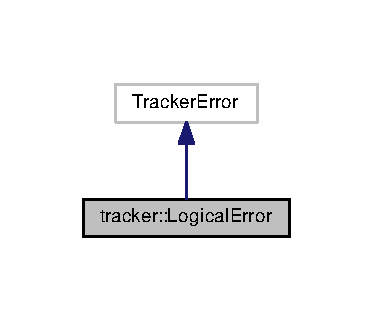
\includegraphics[width=179pt]{structtracker_1_1LogicalError__inherit__graph}
\end{center}
\end{figure}


Collaboration diagram for tracker\+:\+:Logical\+Error\+:\nopagebreak
\begin{figure}[H]
\begin{center}
\leavevmode
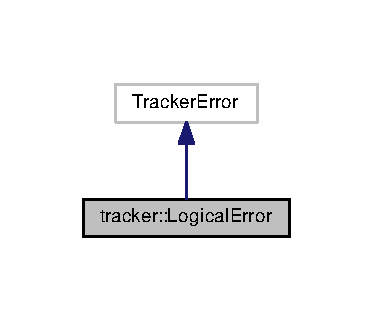
\includegraphics[width=179pt]{structtracker_1_1LogicalError__coll__graph}
\end{center}
\end{figure}
\subsubsection*{Public Member Functions}
\begin{DoxyCompactItemize}
\item 
\hyperlink{structtracker_1_1LogicalError_ac5057f6383f4c192f123d8316cd2044d}{Logical\+Error} (std\+::string message)
\end{DoxyCompactItemize}


\subsubsection{Detailed Description}
Parameter value is not valid. 

Definition at line 40 of file Tracker.\+h.



\subsubsection{Constructor \& Destructor Documentation}
\index{tracker\+::\+Logical\+Error@{tracker\+::\+Logical\+Error}!Logical\+Error@{Logical\+Error}}
\index{Logical\+Error@{Logical\+Error}!tracker\+::\+Logical\+Error@{tracker\+::\+Logical\+Error}}
\paragraph[{\texorpdfstring{Logical\+Error(std\+::string message)}{LogicalError(std::string message)}}]{\setlength{\rightskip}{0pt plus 5cm}tracker\+::\+Logical\+Error\+::\+Logical\+Error (
\begin{DoxyParamCaption}
\item[{std\+::string}]{message}
\end{DoxyParamCaption}
)\hspace{0.3cm}{\ttfamily [inline]}}\hypertarget{structtracker_1_1LogicalError_ac5057f6383f4c192f123d8316cd2044d}{}\label{structtracker_1_1LogicalError_ac5057f6383f4c192f123d8316cd2044d}


Definition at line 42 of file Tracker.\+h.



The documentation for this struct was generated from the following file\+:\begin{DoxyCompactItemize}
\item 
\hyperlink{Tracker_8h}{Tracker.\+h}\end{DoxyCompactItemize}

\hypertarget{structtracker_1_1ParameterValueError}{}\subsection{tracker\+:\+:Parameter\+Value\+Error Struct Reference}
\label{structtracker_1_1ParameterValueError}\index{tracker\+::\+Parameter\+Value\+Error@{tracker\+::\+Parameter\+Value\+Error}}


Parameter value is not valid.  




{\ttfamily \#include $<$/home/travis/build/markjolah/\+Tracker/include/\+Tracker/\+Tracker.\+h$>$}



Inheritance diagram for tracker\+:\+:Parameter\+Value\+Error\+:\nopagebreak
\begin{figure}[H]
\begin{center}
\leavevmode
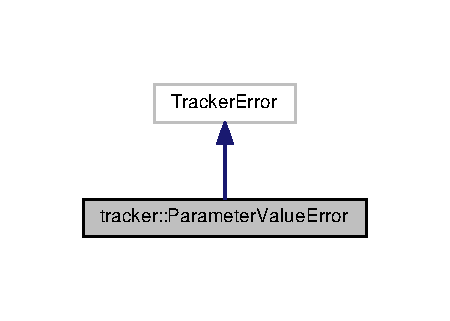
\includegraphics[width=216pt]{structtracker_1_1ParameterValueError__inherit__graph}
\end{center}
\end{figure}


Collaboration diagram for tracker\+:\+:Parameter\+Value\+Error\+:\nopagebreak
\begin{figure}[H]
\begin{center}
\leavevmode
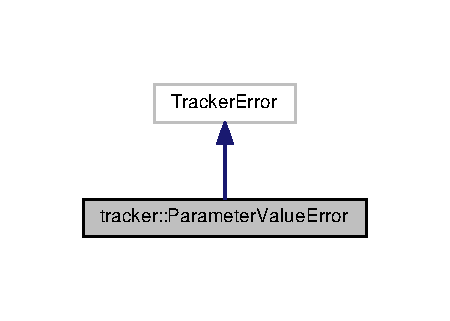
\includegraphics[width=216pt]{structtracker_1_1ParameterValueError__coll__graph}
\end{center}
\end{figure}
\subsubsection*{Public Member Functions}
\begin{DoxyCompactItemize}
\item 
\hyperlink{structtracker_1_1ParameterValueError_a36fc8f74d97839ead3570da53d7a7ba3}{Parameter\+Value\+Error} (std\+::string message)
\end{DoxyCompactItemize}


\subsubsection{Detailed Description}
Parameter value is not valid. 

Definition at line 33 of file Tracker.\+h.



\subsubsection{Constructor \& Destructor Documentation}
\index{tracker\+::\+Parameter\+Value\+Error@{tracker\+::\+Parameter\+Value\+Error}!Parameter\+Value\+Error@{Parameter\+Value\+Error}}
\index{Parameter\+Value\+Error@{Parameter\+Value\+Error}!tracker\+::\+Parameter\+Value\+Error@{tracker\+::\+Parameter\+Value\+Error}}
\paragraph[{\texorpdfstring{Parameter\+Value\+Error(std\+::string message)}{ParameterValueError(std::string message)}}]{\setlength{\rightskip}{0pt plus 5cm}tracker\+::\+Parameter\+Value\+Error\+::\+Parameter\+Value\+Error (
\begin{DoxyParamCaption}
\item[{std\+::string}]{message}
\end{DoxyParamCaption}
)\hspace{0.3cm}{\ttfamily [inline]}}\hypertarget{structtracker_1_1ParameterValueError_a36fc8f74d97839ead3570da53d7a7ba3}{}\label{structtracker_1_1ParameterValueError_a36fc8f74d97839ead3570da53d7a7ba3}


Definition at line 35 of file Tracker.\+h.



The documentation for this struct was generated from the following file\+:\begin{DoxyCompactItemize}
\item 
\hyperlink{Tracker_8h}{Tracker.\+h}\end{DoxyCompactItemize}

\hypertarget{classtracker_1_1Tracker}{}\subsection{tracker\+:\+:Tracker Class Reference}
\label{classtracker_1_1Tracker}\index{tracker\+::\+Tracker@{tracker\+::\+Tracker}}


{\ttfamily \#include $<$/home/travis/build/markjolah/\+Tracker/include/\+Tracker/\+Tracker.\+h$>$}



Inheritance diagram for tracker\+:\+:Tracker\+:\nopagebreak
\begin{figure}[H]
\begin{center}
\leavevmode
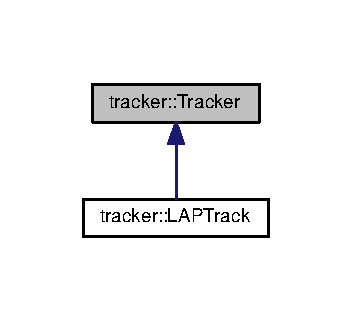
\includegraphics[width=169pt]{classtracker_1_1Tracker__inherit__graph}
\end{center}
\end{figure}


Collaboration diagram for tracker\+:\+:Tracker\+:\nopagebreak
\begin{figure}[H]
\begin{center}
\leavevmode
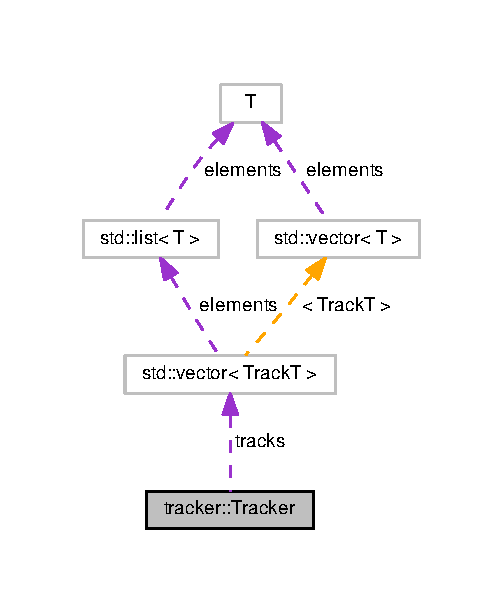
\includegraphics[width=242pt]{classtracker_1_1Tracker__coll__graph}
\end{center}
\end{figure}
\subsubsection*{Public Types}
\begin{DoxyCompactItemize}
\item 
using \hyperlink{classtracker_1_1Tracker_a66e8a81f12871e23082264c964f8f103}{FloatT} = double
\item 
using \hyperlink{classtracker_1_1Tracker_ad39a875dc6957cb6a9f3affcf6517d80}{IdxT} = int32\+\_\+t
\item 
using \hyperlink{classtracker_1_1Tracker_a9905fa9b81b252716e651d87d7d57aff}{VecT} = arma\+::\+Col$<$ \hyperlink{classtracker_1_1Tracker_a66e8a81f12871e23082264c964f8f103}{FloatT} $>$
\item 
using \hyperlink{classtracker_1_1Tracker_a60a1d6ee07284ba82f0533c79311ccfd}{MatT} = arma\+::\+Mat$<$ \hyperlink{classtracker_1_1Tracker_a66e8a81f12871e23082264c964f8f103}{FloatT} $>$
\item 
using \hyperlink{classtracker_1_1Tracker_a59a6e01be987f9c0093a8ac5ad97ce33}{I\+VecT} = arma\+::\+Col$<$ \hyperlink{classtracker_1_1Tracker_ad39a875dc6957cb6a9f3affcf6517d80}{IdxT} $>$
\item 
using \hyperlink{classtracker_1_1Tracker_a6de023cd3b5466996624c7e1b7e5d551}{I\+MatT} = arma\+::\+Mat$<$ \hyperlink{classtracker_1_1Tracker_ad39a875dc6957cb6a9f3affcf6517d80}{IdxT} $>$
\item 
using \hyperlink{classtracker_1_1Tracker_a122e1d351fcb4444aec9729cf7625322}{I\+Vec\+FieldT} = arma\+::field$<$ \hyperlink{classtracker_1_1Tracker_a59a6e01be987f9c0093a8ac5ad97ce33}{I\+VecT} $>$
\item 
using \hyperlink{classtracker_1_1Tracker_a50ae514521f940c08813b45f53b6ce2d}{Index\+VectorT} = std\+::vector$<$ \hyperlink{classtracker_1_1Tracker_ad39a875dc6957cb6a9f3affcf6517d80}{IdxT} $>$
\item 
using \hyperlink{classtracker_1_1Tracker_ac1b06aee1b9d85fb75cf6a9579eb0e84}{TrackT} = std\+::list$<$ \hyperlink{classtracker_1_1Tracker_ad39a875dc6957cb6a9f3affcf6517d80}{IdxT} $>$
\item 
using \hyperlink{classtracker_1_1Tracker_a25ee8479eb10f1619a8eefd5d310eeb7}{Track\+VecT} = std\+::vector$<$ \hyperlink{classtracker_1_1Tracker_ac1b06aee1b9d85fb75cf6a9579eb0e84}{TrackT} $>$
\item 
using \hyperlink{classtracker_1_1Tracker_a5fd443ec1139ed82910dd16316100db7}{ParamT} = std\+::map$<$ std\+::string, \hyperlink{classtracker_1_1Tracker_a66e8a81f12871e23082264c964f8f103}{FloatT} $>$
\item 
using \hyperlink{classtracker_1_1Tracker_a1a79f7073d8e1a032369dcc8105604ce}{Vec\+ParamT} = std\+::map$<$ std\+::string, \hyperlink{classtracker_1_1Tracker_a9905fa9b81b252716e651d87d7d57aff}{VecT} $>$
\end{DoxyCompactItemize}
\subsubsection*{Public Member Functions}
\begin{DoxyCompactItemize}
\item 
\hyperlink{classtracker_1_1Tracker_a27dea2aecabed66961d6d27b7a217d49}{Tracker} (const \hyperlink{classtracker_1_1Tracker_a1a79f7073d8e1a032369dcc8105604ce}{Vec\+ParamT} \&param)
\item 
virtual \hyperlink{classtracker_1_1Tracker_ab443f280a09da7d955e5e963a64b43cf}{$\sim$\+Tracker} ()
\item 
virtual \hyperlink{classtracker_1_1Tracker_a1a79f7073d8e1a032369dcc8105604ce}{Vec\+ParamT} \hyperlink{classtracker_1_1Tracker_a0ff525214ca14a98bacb8af427000cfa}{get\+Stats} () const 
\item 
virtual void \hyperlink{classtracker_1_1Tracker_a54cebc540275536380aca0d9ecb7e575}{initialize\+Tracks} (const \hyperlink{classtracker_1_1Tracker_a59a6e01be987f9c0093a8ac5ad97ce33}{I\+VecT} \&frame\+Idx\+\_\+, const \hyperlink{classtracker_1_1Tracker_a60a1d6ee07284ba82f0533c79311ccfd}{MatT} \&position\+\_\+, const \hyperlink{classtracker_1_1Tracker_a60a1d6ee07284ba82f0533c79311ccfd}{MatT} \&S\+E\+\_\+position\+\_\+)
\item 
virtual void \hyperlink{classtracker_1_1Tracker_a9fbf44fc368d294b47cd3bc48c0c69bd}{initialize\+Tracks} (const \hyperlink{classtracker_1_1Tracker_a59a6e01be987f9c0093a8ac5ad97ce33}{I\+VecT} \&frame\+Idx\+\_\+, const \hyperlink{classtracker_1_1Tracker_a60a1d6ee07284ba82f0533c79311ccfd}{MatT} \&position\+\_\+, const \hyperlink{classtracker_1_1Tracker_a60a1d6ee07284ba82f0533c79311ccfd}{MatT} \&S\+E\+\_\+position\+\_\+, const \hyperlink{classtracker_1_1Tracker_a60a1d6ee07284ba82f0533c79311ccfd}{MatT} \&feature\+\_\+, const \hyperlink{classtracker_1_1Tracker_a60a1d6ee07284ba82f0533c79311ccfd}{MatT} \&S\+E\+\_\+feature\+\_\+)
\item 
virtual void \hyperlink{classtracker_1_1Tracker_a14823a45c80086192c92aa90eb58ca17}{generate\+Tracks} ()=0
\item 
void \hyperlink{classtracker_1_1Tracker_a5d1d2a969102d181b69b23333c874fc3}{print\+Tracks} () const 
\end{DoxyCompactItemize}
\subsubsection*{Public Attributes}
\begin{DoxyCompactItemize}
\item 
\hyperlink{classtracker_1_1Tracker_ad39a875dc6957cb6a9f3affcf6517d80}{IdxT} \hyperlink{classtracker_1_1Tracker_a5d8cb7831463035649c791311001228f}{N} = 0
\item 
\hyperlink{classtracker_1_1Tracker_ad39a875dc6957cb6a9f3affcf6517d80}{IdxT} \hyperlink{classtracker_1_1Tracker_a5efb17589760984816411fb6f69d561d}{n\+Dims} = 0
\item 
\hyperlink{classtracker_1_1Tracker_ad39a875dc6957cb6a9f3affcf6517d80}{IdxT} \hyperlink{classtracker_1_1Tracker_ade0b77f0b5ffc71aecddc70593ec16bb}{n\+Features} = 0
\item 
\hyperlink{classtracker_1_1Tracker_a59a6e01be987f9c0093a8ac5ad97ce33}{I\+VecT} \hyperlink{classtracker_1_1Tracker_aa3e32ff8183fe70af1d351f6324e7615}{frame\+Idx}
\item 
\hyperlink{classtracker_1_1Tracker_a60a1d6ee07284ba82f0533c79311ccfd}{MatT} \hyperlink{classtracker_1_1Tracker_a89978ed5ec72607820f45f3dcf63dd04}{position}
\item 
\hyperlink{classtracker_1_1Tracker_a60a1d6ee07284ba82f0533c79311ccfd}{MatT} \hyperlink{classtracker_1_1Tracker_acd4e8651a05dff9170230149b7fe0029}{S\+E\+\_\+position}
\item 
\hyperlink{classtracker_1_1Tracker_a60a1d6ee07284ba82f0533c79311ccfd}{MatT} \hyperlink{classtracker_1_1Tracker_ab9d6c09e4ae84ff482cd21cc32878138}{feature}
\item 
\hyperlink{classtracker_1_1Tracker_a60a1d6ee07284ba82f0533c79311ccfd}{MatT} \hyperlink{classtracker_1_1Tracker_a0aa2719b06bfd7b630628486b67ca5fd}{S\+E\+\_\+feature}
\item 
\hyperlink{classtracker_1_1Tracker_ad39a875dc6957cb6a9f3affcf6517d80}{IdxT} \hyperlink{classtracker_1_1Tracker_a3ba78a0a502bd2ac432601fc204e3ba1}{first\+Frame} = 0
\item 
\hyperlink{classtracker_1_1Tracker_ad39a875dc6957cb6a9f3affcf6517d80}{IdxT} \hyperlink{classtracker_1_1Tracker_af3219a1e02551ca5c6aafc4a8c14ff30}{last\+Frame} = 0
\item 
\hyperlink{classtracker_1_1Tracker_ad39a875dc6957cb6a9f3affcf6517d80}{IdxT} \hyperlink{classtracker_1_1Tracker_a103afa608ae5693103d81e040a9e29d6}{n\+Frames} = 0
\item 
\hyperlink{classtracker_1_1Tracker_a59a6e01be987f9c0093a8ac5ad97ce33}{I\+VecT} \hyperlink{classtracker_1_1Tracker_a84d3000b7a2b7a2566791f05d3b8afcb}{n\+Frame\+Locs}
\item 
\hyperlink{classtracker_1_1Tracker_a122e1d351fcb4444aec9729cf7625322}{I\+Vec\+FieldT} \hyperlink{classtracker_1_1Tracker_a089a3af55a168691f56d856658786159}{frame\+Loc\+Idx}
\item 
\hyperlink{classtracker_1_1Tracker_a25ee8479eb10f1619a8eefd5d310eeb7}{Track\+VecT} \hyperlink{classtracker_1_1Tracker_a1e43335eb50e56014399a157b261160b}{tracks}
\end{DoxyCompactItemize}
\subsubsection*{Protected Attributes}
\begin{DoxyCompactItemize}
\item 
\hyperlink{classtracker_1_1Tracker_a59a6e01be987f9c0093a8ac5ad97ce33}{I\+VecT} \hyperlink{classtracker_1_1Tracker_a638ecbd5a6466c2730e7c7b9561e9fc9}{track\+Assignment}
\end{DoxyCompactItemize}
\subsubsection*{Static Protected Attributes}
\begin{DoxyCompactItemize}
\item 
static const \hyperlink{classtracker_1_1Tracker_a66e8a81f12871e23082264c964f8f103}{FloatT} \hyperlink{classtracker_1_1Tracker_adf40b4f798f070419f5eb697b36b65ac}{log2pi} = log(2$\ast$arma\+::\+Datum$<$\hyperlink{classtracker_1_1Tracker_a66e8a81f12871e23082264c964f8f103}{Tracker\+::\+FloatT}$>$\+::pi)
\end{DoxyCompactItemize}


\subsubsection{Detailed Description}


Definition at line 45 of file Tracker.\+h.



\subsubsection{Member Typedef Documentation}
\index{tracker\+::\+Tracker@{tracker\+::\+Tracker}!FloatT@{FloatT}}
\index{FloatT@{FloatT}!tracker\+::\+Tracker@{tracker\+::\+Tracker}}
\paragraph[{\texorpdfstring{FloatT}{FloatT}}]{\setlength{\rightskip}{0pt plus 5cm}using {\bf tracker\+::\+Tracker\+::\+FloatT} =  double}\hypertarget{classtracker_1_1Tracker_a66e8a81f12871e23082264c964f8f103}{}\label{classtracker_1_1Tracker_a66e8a81f12871e23082264c964f8f103}


Definition at line 47 of file Tracker.\+h.

\index{tracker\+::\+Tracker@{tracker\+::\+Tracker}!IdxT@{IdxT}}
\index{IdxT@{IdxT}!tracker\+::\+Tracker@{tracker\+::\+Tracker}}
\paragraph[{\texorpdfstring{IdxT}{IdxT}}]{\setlength{\rightskip}{0pt plus 5cm}using {\bf tracker\+::\+Tracker\+::\+IdxT} =  int32\+\_\+t}\hypertarget{classtracker_1_1Tracker_ad39a875dc6957cb6a9f3affcf6517d80}{}\label{classtracker_1_1Tracker_ad39a875dc6957cb6a9f3affcf6517d80}


Definition at line 48 of file Tracker.\+h.

\index{tracker\+::\+Tracker@{tracker\+::\+Tracker}!I\+MatT@{I\+MatT}}
\index{I\+MatT@{I\+MatT}!tracker\+::\+Tracker@{tracker\+::\+Tracker}}
\paragraph[{\texorpdfstring{I\+MatT}{IMatT}}]{\setlength{\rightskip}{0pt plus 5cm}using {\bf tracker\+::\+Tracker\+::\+I\+MatT} =  arma\+::\+Mat$<${\bf IdxT}$>$}\hypertarget{classtracker_1_1Tracker_a6de023cd3b5466996624c7e1b7e5d551}{}\label{classtracker_1_1Tracker_a6de023cd3b5466996624c7e1b7e5d551}


Definition at line 52 of file Tracker.\+h.

\index{tracker\+::\+Tracker@{tracker\+::\+Tracker}!Index\+VectorT@{Index\+VectorT}}
\index{Index\+VectorT@{Index\+VectorT}!tracker\+::\+Tracker@{tracker\+::\+Tracker}}
\paragraph[{\texorpdfstring{Index\+VectorT}{IndexVectorT}}]{\setlength{\rightskip}{0pt plus 5cm}using {\bf tracker\+::\+Tracker\+::\+Index\+VectorT} =  std\+::vector$<${\bf IdxT}$>$}\hypertarget{classtracker_1_1Tracker_a50ae514521f940c08813b45f53b6ce2d}{}\label{classtracker_1_1Tracker_a50ae514521f940c08813b45f53b6ce2d}


Definition at line 54 of file Tracker.\+h.

\index{tracker\+::\+Tracker@{tracker\+::\+Tracker}!I\+Vec\+FieldT@{I\+Vec\+FieldT}}
\index{I\+Vec\+FieldT@{I\+Vec\+FieldT}!tracker\+::\+Tracker@{tracker\+::\+Tracker}}
\paragraph[{\texorpdfstring{I\+Vec\+FieldT}{IVecFieldT}}]{\setlength{\rightskip}{0pt plus 5cm}using {\bf tracker\+::\+Tracker\+::\+I\+Vec\+FieldT} =  arma\+::field$<${\bf I\+VecT}$>$}\hypertarget{classtracker_1_1Tracker_a122e1d351fcb4444aec9729cf7625322}{}\label{classtracker_1_1Tracker_a122e1d351fcb4444aec9729cf7625322}


Definition at line 53 of file Tracker.\+h.

\index{tracker\+::\+Tracker@{tracker\+::\+Tracker}!I\+VecT@{I\+VecT}}
\index{I\+VecT@{I\+VecT}!tracker\+::\+Tracker@{tracker\+::\+Tracker}}
\paragraph[{\texorpdfstring{I\+VecT}{IVecT}}]{\setlength{\rightskip}{0pt plus 5cm}using {\bf tracker\+::\+Tracker\+::\+I\+VecT} =  arma\+::\+Col$<${\bf IdxT}$>$}\hypertarget{classtracker_1_1Tracker_a59a6e01be987f9c0093a8ac5ad97ce33}{}\label{classtracker_1_1Tracker_a59a6e01be987f9c0093a8ac5ad97ce33}


Definition at line 51 of file Tracker.\+h.

\index{tracker\+::\+Tracker@{tracker\+::\+Tracker}!MatT@{MatT}}
\index{MatT@{MatT}!tracker\+::\+Tracker@{tracker\+::\+Tracker}}
\paragraph[{\texorpdfstring{MatT}{MatT}}]{\setlength{\rightskip}{0pt plus 5cm}using {\bf tracker\+::\+Tracker\+::\+MatT} =  arma\+::\+Mat$<${\bf FloatT}$>$}\hypertarget{classtracker_1_1Tracker_a60a1d6ee07284ba82f0533c79311ccfd}{}\label{classtracker_1_1Tracker_a60a1d6ee07284ba82f0533c79311ccfd}


Definition at line 50 of file Tracker.\+h.

\index{tracker\+::\+Tracker@{tracker\+::\+Tracker}!ParamT@{ParamT}}
\index{ParamT@{ParamT}!tracker\+::\+Tracker@{tracker\+::\+Tracker}}
\paragraph[{\texorpdfstring{ParamT}{ParamT}}]{\setlength{\rightskip}{0pt plus 5cm}using {\bf tracker\+::\+Tracker\+::\+ParamT} =  std\+::map$<$std\+::string,{\bf FloatT}$>$}\hypertarget{classtracker_1_1Tracker_a5fd443ec1139ed82910dd16316100db7}{}\label{classtracker_1_1Tracker_a5fd443ec1139ed82910dd16316100db7}
A convenient form for reporting dictionaries of named FP data to matlab 

Definition at line 57 of file Tracker.\+h.

\index{tracker\+::\+Tracker@{tracker\+::\+Tracker}!TrackT@{TrackT}}
\index{TrackT@{TrackT}!tracker\+::\+Tracker@{tracker\+::\+Tracker}}
\paragraph[{\texorpdfstring{TrackT}{TrackT}}]{\setlength{\rightskip}{0pt plus 5cm}using {\bf tracker\+::\+Tracker\+::\+TrackT} =  std\+::list$<${\bf IdxT}$>$}\hypertarget{classtracker_1_1Tracker_ac1b06aee1b9d85fb75cf6a9579eb0e84}{}\label{classtracker_1_1Tracker_ac1b06aee1b9d85fb75cf6a9579eb0e84}
A type for an individual track 

Definition at line 55 of file Tracker.\+h.

\index{tracker\+::\+Tracker@{tracker\+::\+Tracker}!Track\+VecT@{Track\+VecT}}
\index{Track\+VecT@{Track\+VecT}!tracker\+::\+Tracker@{tracker\+::\+Tracker}}
\paragraph[{\texorpdfstring{Track\+VecT}{TrackVecT}}]{\setlength{\rightskip}{0pt plus 5cm}using {\bf tracker\+::\+Tracker\+::\+Track\+VecT} =  std\+::vector$<${\bf TrackT}$>$}\hypertarget{classtracker_1_1Tracker_a25ee8479eb10f1619a8eefd5d310eeb7}{}\label{classtracker_1_1Tracker_a25ee8479eb10f1619a8eefd5d310eeb7}
A type for a vector of tracks 

Definition at line 56 of file Tracker.\+h.

\index{tracker\+::\+Tracker@{tracker\+::\+Tracker}!Vec\+ParamT@{Vec\+ParamT}}
\index{Vec\+ParamT@{Vec\+ParamT}!tracker\+::\+Tracker@{tracker\+::\+Tracker}}
\paragraph[{\texorpdfstring{Vec\+ParamT}{VecParamT}}]{\setlength{\rightskip}{0pt plus 5cm}using {\bf tracker\+::\+Tracker\+::\+Vec\+ParamT} =  std\+::map$<$std\+::string,{\bf VecT}$>$}\hypertarget{classtracker_1_1Tracker_a1a79f7073d8e1a032369dcc8105604ce}{}\label{classtracker_1_1Tracker_a1a79f7073d8e1a032369dcc8105604ce}
A convenient form for reporting dictionaries of named FP data to matlab 

Definition at line 58 of file Tracker.\+h.

\index{tracker\+::\+Tracker@{tracker\+::\+Tracker}!VecT@{VecT}}
\index{VecT@{VecT}!tracker\+::\+Tracker@{tracker\+::\+Tracker}}
\paragraph[{\texorpdfstring{VecT}{VecT}}]{\setlength{\rightskip}{0pt plus 5cm}using {\bf tracker\+::\+Tracker\+::\+VecT} =  arma\+::\+Col$<${\bf FloatT}$>$}\hypertarget{classtracker_1_1Tracker_a9905fa9b81b252716e651d87d7d57aff}{}\label{classtracker_1_1Tracker_a9905fa9b81b252716e651d87d7d57aff}


Definition at line 49 of file Tracker.\+h.



\subsubsection{Constructor \& Destructor Documentation}
\index{tracker\+::\+Tracker@{tracker\+::\+Tracker}!Tracker@{Tracker}}
\index{Tracker@{Tracker}!tracker\+::\+Tracker@{tracker\+::\+Tracker}}
\paragraph[{\texorpdfstring{Tracker(const Vec\+Param\+T \&param)}{Tracker(const VecParamT &param)}}]{\setlength{\rightskip}{0pt plus 5cm}tracker\+::\+Tracker\+::\+Tracker (
\begin{DoxyParamCaption}
\item[{const {\bf Vec\+ParamT} \&}]{param}
\end{DoxyParamCaption}
)}\hypertarget{classtracker_1_1Tracker_a27dea2aecabed66961d6d27b7a217d49}{}\label{classtracker_1_1Tracker_a27dea2aecabed66961d6d27b7a217d49}
param -\/ A dictionary of floating point values to pass in. This is a flexible interface to the higher-\/level matlab code allowing each subclass to take in arbitrary floating point arguments. 

Definition at line 15 of file Tracker.\+cpp.

\index{tracker\+::\+Tracker@{tracker\+::\+Tracker}!````~Tracker@{$\sim$\+Tracker}}
\index{````~Tracker@{$\sim$\+Tracker}!tracker\+::\+Tracker@{tracker\+::\+Tracker}}
\paragraph[{\texorpdfstring{$\sim$\+Tracker()}{~Tracker()}}]{\setlength{\rightskip}{0pt plus 5cm}virtual tracker\+::\+Tracker\+::$\sim$\+Tracker (
\begin{DoxyParamCaption}
{}
\end{DoxyParamCaption}
)\hspace{0.3cm}{\ttfamily [inline]}, {\ttfamily [virtual]}}\hypertarget{classtracker_1_1Tracker_ab443f280a09da7d955e5e963a64b43cf}{}\label{classtracker_1_1Tracker_ab443f280a09da7d955e5e963a64b43cf}


Definition at line 84 of file Tracker.\+h.



\subsubsection{Member Function Documentation}
\index{tracker\+::\+Tracker@{tracker\+::\+Tracker}!generate\+Tracks@{generate\+Tracks}}
\index{generate\+Tracks@{generate\+Tracks}!tracker\+::\+Tracker@{tracker\+::\+Tracker}}
\paragraph[{\texorpdfstring{generate\+Tracks()=0}{generateTracks()=0}}]{\setlength{\rightskip}{0pt plus 5cm}virtual void tracker\+::\+Tracker\+::generate\+Tracks (
\begin{DoxyParamCaption}
{}
\end{DoxyParamCaption}
)\hspace{0.3cm}{\ttfamily [pure virtual]}}\hypertarget{classtracker_1_1Tracker_a14823a45c80086192c92aa90eb58ca17}{}\label{classtracker_1_1Tracker_a14823a45c80086192c92aa90eb58ca17}


Implemented in \hyperlink{classtracker_1_1LAPTrack_aac61350c9f3e2c12c9aef7892a718f38}{tracker\+::\+L\+A\+P\+Track}.

\index{tracker\+::\+Tracker@{tracker\+::\+Tracker}!get\+Stats@{get\+Stats}}
\index{get\+Stats@{get\+Stats}!tracker\+::\+Tracker@{tracker\+::\+Tracker}}
\paragraph[{\texorpdfstring{get\+Stats() const }{getStats() const }}]{\setlength{\rightskip}{0pt plus 5cm}{\bf Tracker\+::\+Vec\+ParamT} tracker\+::\+Tracker\+::get\+Stats (
\begin{DoxyParamCaption}
{}
\end{DoxyParamCaption}
) const\hspace{0.3cm}{\ttfamily [virtual]}}\hypertarget{classtracker_1_1Tracker_a0ff525214ca14a98bacb8af427000cfa}{}\label{classtracker_1_1Tracker_a0ff525214ca14a98bacb8af427000cfa}


Reimplemented in \hyperlink{classtracker_1_1LAPTrack_ab5dc7bdfbaafa9eafec4d9fd7ade3411}{tracker\+::\+L\+A\+P\+Track}.



Definition at line 19 of file Tracker.\+cpp.



References first\+Frame, last\+Frame, N, n\+Dims, n\+Features, n\+Frames, track\+Assignment, and tracks.



Referenced by tracker\+::\+L\+A\+P\+Track\+::get\+Stats().



Here is the caller graph for this function\+:\nopagebreak
\begin{figure}[H]
\begin{center}
\leavevmode
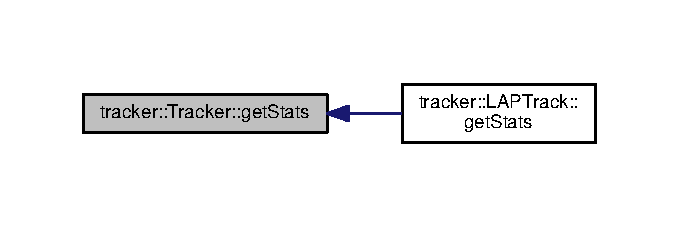
\includegraphics[width=326pt]{classtracker_1_1Tracker_a0ff525214ca14a98bacb8af427000cfa_icgraph}
\end{center}
\end{figure}


\index{tracker\+::\+Tracker@{tracker\+::\+Tracker}!initialize\+Tracks@{initialize\+Tracks}}
\index{initialize\+Tracks@{initialize\+Tracks}!tracker\+::\+Tracker@{tracker\+::\+Tracker}}
\paragraph[{\texorpdfstring{initialize\+Tracks(const I\+Vec\+T \&frame\+Idx\+\_\+, const Mat\+T \&position\+\_\+, const Mat\+T \&\+S\+E\+\_\+position\+\_\+)}{initializeTracks(const IVecT &frameIdx_, const MatT &position_, const MatT &SE_position_)}}]{\setlength{\rightskip}{0pt plus 5cm}void tracker\+::\+Tracker\+::initialize\+Tracks (
\begin{DoxyParamCaption}
\item[{const {\bf I\+VecT} \&}]{frame\+Idx\+\_\+, }
\item[{const {\bf MatT} \&}]{position\+\_\+, }
\item[{const {\bf MatT} \&}]{S\+E\+\_\+position\+\_\+}
\end{DoxyParamCaption}
)\hspace{0.3cm}{\ttfamily [virtual]}}\hypertarget{classtracker_1_1Tracker_a54cebc540275536380aca0d9ecb7e575}{}\label{classtracker_1_1Tracker_a54cebc540275536380aca0d9ecb7e575}


Reimplemented in \hyperlink{classtracker_1_1LAPTrack_a9561d939e76b3ed9afca03cc4d457c9e}{tracker\+::\+L\+A\+P\+Track}.



Definition at line 33 of file Tracker.\+cpp.



Referenced by tracker\+::\+L\+A\+P\+Track\+::initialize\+Tracks().



Here is the caller graph for this function\+:\nopagebreak
\begin{figure}[H]
\begin{center}
\leavevmode
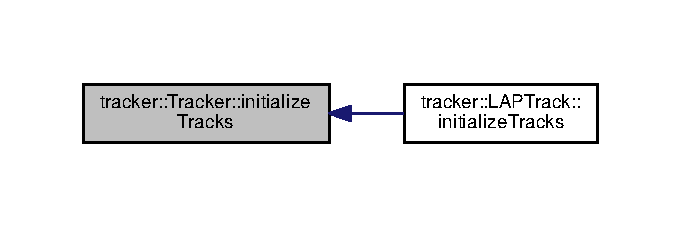
\includegraphics[width=327pt]{classtracker_1_1Tracker_a54cebc540275536380aca0d9ecb7e575_icgraph}
\end{center}
\end{figure}


\index{tracker\+::\+Tracker@{tracker\+::\+Tracker}!initialize\+Tracks@{initialize\+Tracks}}
\index{initialize\+Tracks@{initialize\+Tracks}!tracker\+::\+Tracker@{tracker\+::\+Tracker}}
\paragraph[{\texorpdfstring{initialize\+Tracks(const I\+Vec\+T \&frame\+Idx\+\_\+, const Mat\+T \&position\+\_\+, const Mat\+T \&\+S\+E\+\_\+position\+\_\+, const Mat\+T \&feature\+\_\+, const Mat\+T \&\+S\+E\+\_\+feature\+\_\+)}{initializeTracks(const IVecT &frameIdx_, const MatT &position_, const MatT &SE_position_, const MatT &feature_, const MatT &SE_feature_)}}]{\setlength{\rightskip}{0pt plus 5cm}void tracker\+::\+Tracker\+::initialize\+Tracks (
\begin{DoxyParamCaption}
\item[{const {\bf I\+VecT} \&}]{frame\+Idx\+\_\+, }
\item[{const {\bf MatT} \&}]{position\+\_\+, }
\item[{const {\bf MatT} \&}]{S\+E\+\_\+position\+\_\+, }
\item[{const {\bf MatT} \&}]{feature\+\_\+, }
\item[{const {\bf MatT} \&}]{S\+E\+\_\+feature\+\_\+}
\end{DoxyParamCaption}
)\hspace{0.3cm}{\ttfamily [virtual]}}\hypertarget{classtracker_1_1Tracker_a9fbf44fc368d294b47cd3bc48c0c69bd}{}\label{classtracker_1_1Tracker_a9fbf44fc368d294b47cd3bc48c0c69bd}


Reimplemented in \hyperlink{classtracker_1_1LAPTrack_a22ba01a68c707be9b3e906e14b84ff1f}{tracker\+::\+L\+A\+P\+Track}.



Definition at line 39 of file Tracker.\+cpp.



References feature, first\+Frame, frame\+Idx, frame\+Loc\+Idx, last\+Frame, N, n\+Dims, n\+Features, n\+Frame\+Locs, n\+Frames, position, S\+E\+\_\+feature, S\+E\+\_\+position, track\+Assignment, and tracks.

\index{tracker\+::\+Tracker@{tracker\+::\+Tracker}!print\+Tracks@{print\+Tracks}}
\index{print\+Tracks@{print\+Tracks}!tracker\+::\+Tracker@{tracker\+::\+Tracker}}
\paragraph[{\texorpdfstring{print\+Tracks() const }{printTracks() const }}]{\setlength{\rightskip}{0pt plus 5cm}void tracker\+::\+Tracker\+::print\+Tracks (
\begin{DoxyParamCaption}
{}
\end{DoxyParamCaption}
) const}\hypertarget{classtracker_1_1Tracker_a5d1d2a969102d181b69b23333c874fc3}{}\label{classtracker_1_1Tracker_a5d1d2a969102d181b69b23333c874fc3}


Definition at line 126 of file Tracker.\+cpp.



References frame\+Idx, and tracks.



\subsubsection{Member Data Documentation}
\index{tracker\+::\+Tracker@{tracker\+::\+Tracker}!feature@{feature}}
\index{feature@{feature}!tracker\+::\+Tracker@{tracker\+::\+Tracker}}
\paragraph[{\texorpdfstring{feature}{feature}}]{\setlength{\rightskip}{0pt plus 5cm}{\bf MatT} tracker\+::\+Tracker\+::feature}\hypertarget{classtracker_1_1Tracker_ab9d6c09e4ae84ff482cd21cc32878138}{}\label{classtracker_1_1Tracker_ab9d6c09e4ae84ff482cd21cc32878138}


Definition at line 66 of file Tracker.\+h.



Referenced by tracker\+::\+L\+A\+P\+Track\+::compute\+F2\+F\+Cost\+Mat(), tracker\+::\+L\+A\+P\+Track\+::compute\+Gap\+Close\+Matrix(), and initialize\+Tracks().

\index{tracker\+::\+Tracker@{tracker\+::\+Tracker}!first\+Frame@{first\+Frame}}
\index{first\+Frame@{first\+Frame}!tracker\+::\+Tracker@{tracker\+::\+Tracker}}
\paragraph[{\texorpdfstring{first\+Frame}{firstFrame}}]{\setlength{\rightskip}{0pt plus 5cm}{\bf IdxT} tracker\+::\+Tracker\+::first\+Frame = 0}\hypertarget{classtracker_1_1Tracker_a3ba78a0a502bd2ac432601fc204e3ba1}{}\label{classtracker_1_1Tracker_a3ba78a0a502bd2ac432601fc204e3ba1}


Definition at line 68 of file Tracker.\+h.



Referenced by tracker\+::\+L\+A\+P\+Track\+::check\+Frame\+Idxs(), tracker\+::\+L\+A\+P\+Track\+::compute\+F2\+F\+Cost\+Mat(), tracker\+::\+L\+A\+P\+Track\+::compute\+Gap\+Close\+Matrix(), tracker\+::\+L\+A\+P\+Track\+::debug\+F2\+F(), get\+Stats(), initialize\+Tracks(), and tracker\+::\+L\+A\+P\+Track\+::link\+F2\+F().

\index{tracker\+::\+Tracker@{tracker\+::\+Tracker}!frame\+Idx@{frame\+Idx}}
\index{frame\+Idx@{frame\+Idx}!tracker\+::\+Tracker@{tracker\+::\+Tracker}}
\paragraph[{\texorpdfstring{frame\+Idx}{frameIdx}}]{\setlength{\rightskip}{0pt plus 5cm}{\bf I\+VecT} tracker\+::\+Tracker\+::frame\+Idx}\hypertarget{classtracker_1_1Tracker_aa3e32ff8183fe70af1d351f6324e7615}{}\label{classtracker_1_1Tracker_aa3e32ff8183fe70af1d351f6324e7615}


Definition at line 63 of file Tracker.\+h.



Referenced by tracker\+::\+L\+A\+P\+Track\+::check\+Frame\+Idxs(), tracker\+::\+L\+A\+P\+Track\+::compute\+Gap\+Close\+Matrix(), initialize\+Tracks(), and print\+Tracks().

\index{tracker\+::\+Tracker@{tracker\+::\+Tracker}!frame\+Loc\+Idx@{frame\+Loc\+Idx}}
\index{frame\+Loc\+Idx@{frame\+Loc\+Idx}!tracker\+::\+Tracker@{tracker\+::\+Tracker}}
\paragraph[{\texorpdfstring{frame\+Loc\+Idx}{frameLocIdx}}]{\setlength{\rightskip}{0pt plus 5cm}{\bf I\+Vec\+FieldT} tracker\+::\+Tracker\+::frame\+Loc\+Idx}\hypertarget{classtracker_1_1Tracker_a089a3af55a168691f56d856658786159}{}\label{classtracker_1_1Tracker_a089a3af55a168691f56d856658786159}


Definition at line 74 of file Tracker.\+h.



Referenced by tracker\+::\+L\+A\+P\+Track\+::compute\+F2\+F\+Cost\+Mat(), tracker\+::\+L\+A\+P\+Track\+::debug\+F2\+F(), initialize\+Tracks(), and tracker\+::\+L\+A\+P\+Track\+::link\+F2\+F().

\index{tracker\+::\+Tracker@{tracker\+::\+Tracker}!last\+Frame@{last\+Frame}}
\index{last\+Frame@{last\+Frame}!tracker\+::\+Tracker@{tracker\+::\+Tracker}}
\paragraph[{\texorpdfstring{last\+Frame}{lastFrame}}]{\setlength{\rightskip}{0pt plus 5cm}{\bf IdxT} tracker\+::\+Tracker\+::last\+Frame = 0}\hypertarget{classtracker_1_1Tracker_af3219a1e02551ca5c6aafc4a8c14ff30}{}\label{classtracker_1_1Tracker_af3219a1e02551ca5c6aafc4a8c14ff30}


Definition at line 69 of file Tracker.\+h.



Referenced by tracker\+::\+L\+A\+P\+Track\+::check\+Frame\+Idxs(), tracker\+::\+L\+A\+P\+Track\+::compute\+Gap\+Close\+Matrix(), tracker\+::\+L\+A\+P\+Track\+::debug\+F2\+F(), get\+Stats(), initialize\+Tracks(), and tracker\+::\+L\+A\+P\+Track\+::link\+F2\+F().

\index{tracker\+::\+Tracker@{tracker\+::\+Tracker}!log2pi@{log2pi}}
\index{log2pi@{log2pi}!tracker\+::\+Tracker@{tracker\+::\+Tracker}}
\paragraph[{\texorpdfstring{log2pi}{log2pi}}]{\setlength{\rightskip}{0pt plus 5cm}const {\bf Tracker\+::\+FloatT} tracker\+::\+Tracker\+::log2pi = log(2$\ast$arma\+::\+Datum$<${\bf Tracker\+::\+FloatT}$>$\+::pi)\hspace{0.3cm}{\ttfamily [static]}, {\ttfamily [protected]}}\hypertarget{classtracker_1_1Tracker_adf40b4f798f070419f5eb697b36b65ac}{}\label{classtracker_1_1Tracker_adf40b4f798f070419f5eb697b36b65ac}


Definition at line 92 of file Tracker.\+h.



Referenced by tracker\+::\+L\+A\+P\+Track\+::compute\+F2\+F\+Cost\+Mat(), and tracker\+::\+L\+A\+P\+Track\+::compute\+Gap\+Close\+Matrix().

\index{tracker\+::\+Tracker@{tracker\+::\+Tracker}!N@{N}}
\index{N@{N}!tracker\+::\+Tracker@{tracker\+::\+Tracker}}
\paragraph[{\texorpdfstring{N}{N}}]{\setlength{\rightskip}{0pt plus 5cm}{\bf IdxT} tracker\+::\+Tracker\+::N = 0}\hypertarget{classtracker_1_1Tracker_a5d8cb7831463035649c791311001228f}{}\label{classtracker_1_1Tracker_a5d8cb7831463035649c791311001228f}


Definition at line 60 of file Tracker.\+h.



Referenced by get\+Stats(), and initialize\+Tracks().

\index{tracker\+::\+Tracker@{tracker\+::\+Tracker}!n\+Dims@{n\+Dims}}
\index{n\+Dims@{n\+Dims}!tracker\+::\+Tracker@{tracker\+::\+Tracker}}
\paragraph[{\texorpdfstring{n\+Dims}{nDims}}]{\setlength{\rightskip}{0pt plus 5cm}{\bf IdxT} tracker\+::\+Tracker\+::n\+Dims = 0}\hypertarget{classtracker_1_1Tracker_a5efb17589760984816411fb6f69d561d}{}\label{classtracker_1_1Tracker_a5efb17589760984816411fb6f69d561d}


Definition at line 61 of file Tracker.\+h.



Referenced by tracker\+::\+L\+A\+P\+Track\+::compute\+F2\+F\+Cost\+Mat(), tracker\+::\+L\+A\+P\+Track\+::compute\+Gap\+Close\+Matrix(), get\+Stats(), and initialize\+Tracks().

\index{tracker\+::\+Tracker@{tracker\+::\+Tracker}!n\+Features@{n\+Features}}
\index{n\+Features@{n\+Features}!tracker\+::\+Tracker@{tracker\+::\+Tracker}}
\paragraph[{\texorpdfstring{n\+Features}{nFeatures}}]{\setlength{\rightskip}{0pt plus 5cm}{\bf IdxT} tracker\+::\+Tracker\+::n\+Features = 0}\hypertarget{classtracker_1_1Tracker_ade0b77f0b5ffc71aecddc70593ec16bb}{}\label{classtracker_1_1Tracker_ade0b77f0b5ffc71aecddc70593ec16bb}


Definition at line 62 of file Tracker.\+h.



Referenced by tracker\+::\+L\+A\+P\+Track\+::compute\+F2\+F\+Cost\+Mat(), tracker\+::\+L\+A\+P\+Track\+::compute\+Gap\+Close\+Matrix(), get\+Stats(), and initialize\+Tracks().

\index{tracker\+::\+Tracker@{tracker\+::\+Tracker}!n\+Frame\+Locs@{n\+Frame\+Locs}}
\index{n\+Frame\+Locs@{n\+Frame\+Locs}!tracker\+::\+Tracker@{tracker\+::\+Tracker}}
\paragraph[{\texorpdfstring{n\+Frame\+Locs}{nFrameLocs}}]{\setlength{\rightskip}{0pt plus 5cm}{\bf I\+VecT} tracker\+::\+Tracker\+::n\+Frame\+Locs}\hypertarget{classtracker_1_1Tracker_a84d3000b7a2b7a2566791f05d3b8afcb}{}\label{classtracker_1_1Tracker_a84d3000b7a2b7a2566791f05d3b8afcb}


Definition at line 73 of file Tracker.\+h.



Referenced by tracker\+::\+L\+A\+P\+Track\+::compute\+F2\+F\+Cost\+Mat(), tracker\+::\+L\+A\+P\+Track\+::debug\+F2\+F(), initialize\+Tracks(), and tracker\+::\+L\+A\+P\+Track\+::link\+F2\+F().

\index{tracker\+::\+Tracker@{tracker\+::\+Tracker}!n\+Frames@{n\+Frames}}
\index{n\+Frames@{n\+Frames}!tracker\+::\+Tracker@{tracker\+::\+Tracker}}
\paragraph[{\texorpdfstring{n\+Frames}{nFrames}}]{\setlength{\rightskip}{0pt plus 5cm}{\bf IdxT} tracker\+::\+Tracker\+::n\+Frames = 0}\hypertarget{classtracker_1_1Tracker_a103afa608ae5693103d81e040a9e29d6}{}\label{classtracker_1_1Tracker_a103afa608ae5693103d81e040a9e29d6}


Definition at line 70 of file Tracker.\+h.



Referenced by get\+Stats(), initialize\+Tracks(), and tracker\+::\+L\+A\+P\+Track\+::link\+F2\+F().

\index{tracker\+::\+Tracker@{tracker\+::\+Tracker}!position@{position}}
\index{position@{position}!tracker\+::\+Tracker@{tracker\+::\+Tracker}}
\paragraph[{\texorpdfstring{position}{position}}]{\setlength{\rightskip}{0pt plus 5cm}{\bf MatT} tracker\+::\+Tracker\+::position}\hypertarget{classtracker_1_1Tracker_a89978ed5ec72607820f45f3dcf63dd04}{}\label{classtracker_1_1Tracker_a89978ed5ec72607820f45f3dcf63dd04}


Definition at line 64 of file Tracker.\+h.



Referenced by tracker\+::\+L\+A\+P\+Track\+::compute\+F2\+F\+Cost\+Mat(), tracker\+::\+L\+A\+P\+Track\+::compute\+Gap\+Close\+Matrix(), and initialize\+Tracks().

\index{tracker\+::\+Tracker@{tracker\+::\+Tracker}!S\+E\+\_\+feature@{S\+E\+\_\+feature}}
\index{S\+E\+\_\+feature@{S\+E\+\_\+feature}!tracker\+::\+Tracker@{tracker\+::\+Tracker}}
\paragraph[{\texorpdfstring{S\+E\+\_\+feature}{SE_feature}}]{\setlength{\rightskip}{0pt plus 5cm}{\bf MatT} tracker\+::\+Tracker\+::\+S\+E\+\_\+feature}\hypertarget{classtracker_1_1Tracker_a0aa2719b06bfd7b630628486b67ca5fd}{}\label{classtracker_1_1Tracker_a0aa2719b06bfd7b630628486b67ca5fd}


Definition at line 67 of file Tracker.\+h.



Referenced by tracker\+::\+L\+A\+P\+Track\+::compute\+F2\+F\+Cost\+Mat(), tracker\+::\+L\+A\+P\+Track\+::compute\+Gap\+Close\+Matrix(), and initialize\+Tracks().

\index{tracker\+::\+Tracker@{tracker\+::\+Tracker}!S\+E\+\_\+position@{S\+E\+\_\+position}}
\index{S\+E\+\_\+position@{S\+E\+\_\+position}!tracker\+::\+Tracker@{tracker\+::\+Tracker}}
\paragraph[{\texorpdfstring{S\+E\+\_\+position}{SE_position}}]{\setlength{\rightskip}{0pt plus 5cm}{\bf MatT} tracker\+::\+Tracker\+::\+S\+E\+\_\+position}\hypertarget{classtracker_1_1Tracker_acd4e8651a05dff9170230149b7fe0029}{}\label{classtracker_1_1Tracker_acd4e8651a05dff9170230149b7fe0029}


Definition at line 65 of file Tracker.\+h.



Referenced by tracker\+::\+L\+A\+P\+Track\+::compute\+F2\+F\+Cost\+Mat(), tracker\+::\+L\+A\+P\+Track\+::compute\+Gap\+Close\+Matrix(), and initialize\+Tracks().

\index{tracker\+::\+Tracker@{tracker\+::\+Tracker}!track\+Assignment@{track\+Assignment}}
\index{track\+Assignment@{track\+Assignment}!tracker\+::\+Tracker@{tracker\+::\+Tracker}}
\paragraph[{\texorpdfstring{track\+Assignment}{trackAssignment}}]{\setlength{\rightskip}{0pt plus 5cm}{\bf I\+VecT} tracker\+::\+Tracker\+::track\+Assignment\hspace{0.3cm}{\ttfamily [protected]}}\hypertarget{classtracker_1_1Tracker_a638ecbd5a6466c2730e7c7b9561e9fc9}{}\label{classtracker_1_1Tracker_a638ecbd5a6466c2730e7c7b9561e9fc9}


Definition at line 93 of file Tracker.\+h.



Referenced by tracker\+::\+L\+A\+P\+Track\+::close\+Gaps(), get\+Stats(), initialize\+Tracks(), and tracker\+::\+L\+A\+P\+Track\+::link\+F2\+F().

\index{tracker\+::\+Tracker@{tracker\+::\+Tracker}!tracks@{tracks}}
\index{tracks@{tracks}!tracker\+::\+Tracker@{tracker\+::\+Tracker}}
\paragraph[{\texorpdfstring{tracks}{tracks}}]{\setlength{\rightskip}{0pt plus 5cm}{\bf Track\+VecT} tracker\+::\+Tracker\+::tracks}\hypertarget{classtracker_1_1Tracker_a1e43335eb50e56014399a157b261160b}{}\label{classtracker_1_1Tracker_a1e43335eb50e56014399a157b261160b}


Definition at line 77 of file Tracker.\+h.



Referenced by tracker\+::\+L\+A\+P\+Track\+::check\+Frame\+Idxs(), tracker\+::\+L\+A\+P\+Track\+::close\+Gaps(), tracker\+::\+L\+A\+P\+Track\+::compute\+Gap\+Close\+Matrix(), tracker\+::\+L\+A\+P\+Track\+::debug\+Close\+Gaps(), get\+Stats(), initialize\+Tracks(), tracker\+::\+L\+A\+P\+Track\+::link\+F2\+F(), and print\+Tracks().



The documentation for this class was generated from the following files\+:\begin{DoxyCompactItemize}
\item 
\hyperlink{Tracker_8h}{Tracker.\+h}\item 
\hyperlink{Tracker_8cpp}{Tracker.\+cpp}\end{DoxyCompactItemize}

\section{File Documentation}
\hypertarget{LAP__JVSparse_8cpp}{}\subsection{L\+A\+P\+\_\+\+J\+V\+Sparse.\+cpp File Reference}
\label{LAP__JVSparse_8cpp}\index{L\+A\+P\+\_\+\+J\+V\+Sparse.\+cpp@{L\+A\+P\+\_\+\+J\+V\+Sparse.\+cpp}}


The member definitions for the L\+AP Jonker Volgenant algorithm.  


{\ttfamily \#include $<$cmath$>$}\\*
{\ttfamily \#include $<$iostream$>$}\\*
{\ttfamily \#include $<$iomanip$>$}\\*
{\ttfamily \#include \char`\"{}Tracker/\+L\+A\+P\+\_\+\+J\+V\+Sparse.\+h\char`\"{}}\\*
Include dependency graph for L\+A\+P\+\_\+\+J\+V\+Sparse.\+cpp\+:\nopagebreak
\begin{figure}[H]
\begin{center}
\leavevmode
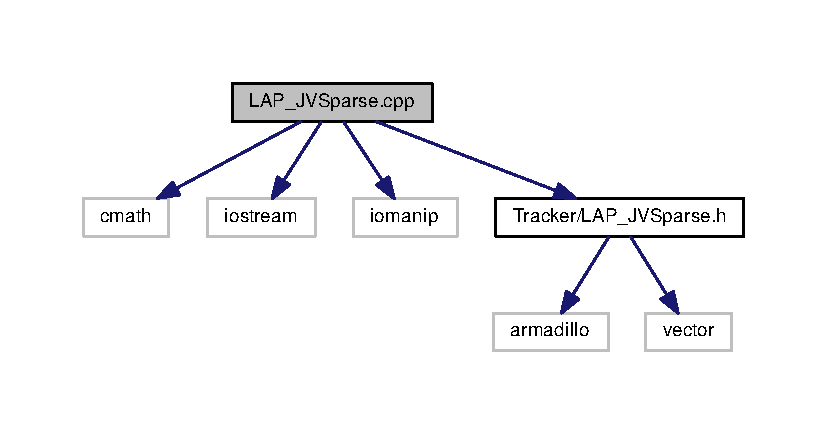
\includegraphics[width=350pt]{LAP__JVSparse_8cpp__incl}
\end{center}
\end{figure}
\subsubsection*{Namespaces}
\begin{DoxyCompactItemize}
\item 
 \hyperlink{namespacetracker}{tracker}
\end{DoxyCompactItemize}


\subsubsection{Detailed Description}
The member definitions for the L\+AP Jonker Volgenant algorithm. 

\begin{DoxyAuthor}{Author}
Mark J. Olah (mjo at cs.\+unm.\+edu) 
\end{DoxyAuthor}
\begin{DoxyDate}{Date}
2015-\/2019 This is a modern dense/sparse C++ implementation of Jonker Volgenant algoirthm using armadillo and presenting C++ and Matlab interface.
\end{DoxyDate}
Adapted from text of Jonker and Volgenant. Computing 38, 324-\/340 (1986) 
\hypertarget{LAP__JVSparse_8h}{}\subsection{L\+A\+P\+\_\+\+J\+V\+Sparse.\+h File Reference}
\label{LAP__JVSparse_8h}\index{L\+A\+P\+\_\+\+J\+V\+Sparse.\+h@{L\+A\+P\+\_\+\+J\+V\+Sparse.\+h}}


The class declaration for the L\+AP Jonker Volgenant algorithm.  


{\ttfamily \#include $<$armadillo$>$}\\*
{\ttfamily \#include $<$vector$>$}\\*
Include dependency graph for L\+A\+P\+\_\+\+J\+V\+Sparse.\+h\+:\nopagebreak
\begin{figure}[H]
\begin{center}
\leavevmode
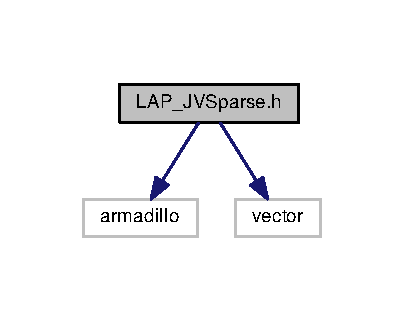
\includegraphics[width=194pt]{LAP__JVSparse_8h__incl}
\end{center}
\end{figure}
This graph shows which files directly or indirectly include this file\+:\nopagebreak
\begin{figure}[H]
\begin{center}
\leavevmode
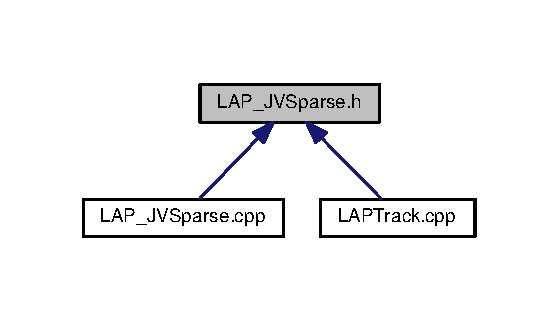
\includegraphics[width=268pt]{LAP__JVSparse_8h__dep__incl}
\end{center}
\end{figure}
\subsubsection*{Classes}
\begin{DoxyCompactItemize}
\item 
class \hyperlink{classtracker_1_1LAP__JVSparse}{tracker\+::\+L\+A\+P\+\_\+\+J\+V\+Sparse$<$ Float\+T $>$}
\end{DoxyCompactItemize}
\subsubsection*{Namespaces}
\begin{DoxyCompactItemize}
\item 
 \hyperlink{namespacetracker}{tracker}
\end{DoxyCompactItemize}


\subsubsection{Detailed Description}
The class declaration for the L\+AP Jonker Volgenant algorithm. 

\begin{DoxyAuthor}{Author}
Mark J. Olah (mjo@cs.\+unm.\+edu) 
\end{DoxyAuthor}
\begin{DoxyDate}{Date}
05-\/2015 This is a modern dense/sparse C++ implementation of Jonker Volgenant algoirthm using armadillo and presenting C++ and Matlab interface.
\end{DoxyDate}
Adapted from text of Jonker and Volgenant. Computing 38, 324-\/340 (1986) 
\hypertarget{LAPTrack_8cpp}{}\subsection{L\+A\+P\+Track.\+cpp File Reference}
\label{LAPTrack_8cpp}\index{L\+A\+P\+Track.\+cpp@{L\+A\+P\+Track.\+cpp}}


The member definitions for L\+A\+P\+Track.  


{\ttfamily \#include \char`\"{}Tracker/\+L\+A\+P\+Track.\+h\char`\"{}}\\*
{\ttfamily \#include \char`\"{}Tracker/\+L\+A\+P\+\_\+\+J\+V\+Sparse.\+h\char`\"{}}\\*
Include dependency graph for L\+A\+P\+Track.\+cpp\+:\nopagebreak
\begin{figure}[H]
\begin{center}
\leavevmode
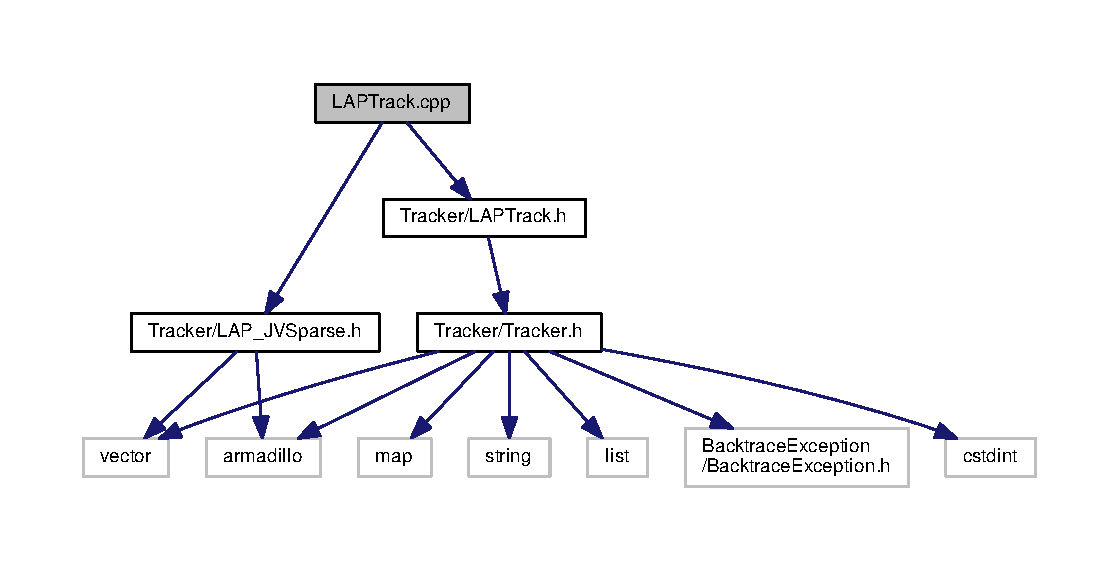
\includegraphics[width=350pt]{LAPTrack_8cpp__incl}
\end{center}
\end{figure}
\subsubsection*{Namespaces}
\begin{DoxyCompactItemize}
\item 
 \hyperlink{namespacetracker}{tracker}
\end{DoxyCompactItemize}


\subsubsection{Detailed Description}
The member definitions for L\+A\+P\+Track. 

\begin{DoxyAuthor}{Author}
Mark J. Olah (mjo at cs.\+unm.\+edu) 
\end{DoxyAuthor}
\begin{DoxyDate}{Date}
2015-\/2019 
\end{DoxyDate}

\hypertarget{LAPTrack_8h}{}\subsection{L\+A\+P\+Track.\+h File Reference}
\label{LAPTrack_8h}\index{L\+A\+P\+Track.\+h@{L\+A\+P\+Track.\+h}}


The class declaration and inline and templated functions for L\+A\+P\+Track.  


{\ttfamily \#include \char`\"{}Tracker/\+Tracker.\+h\char`\"{}}\\*
Include dependency graph for L\+A\+P\+Track.\+h\+:\nopagebreak
\begin{figure}[H]
\begin{center}
\leavevmode
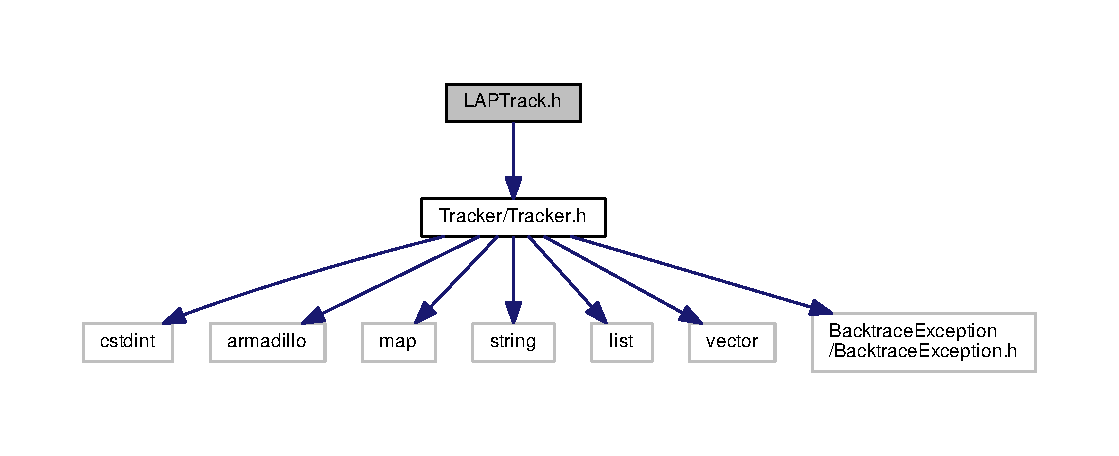
\includegraphics[width=350pt]{LAPTrack_8h__incl}
\end{center}
\end{figure}
This graph shows which files directly or indirectly include this file\+:\nopagebreak
\begin{figure}[H]
\begin{center}
\leavevmode
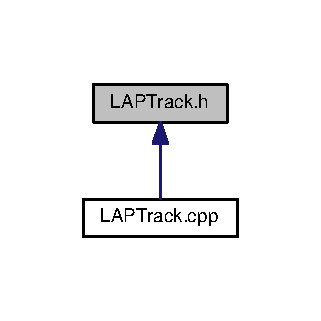
\includegraphics[width=154pt]{LAPTrack_8h__dep__incl}
\end{center}
\end{figure}
\subsubsection*{Classes}
\begin{DoxyCompactItemize}
\item 
class \hyperlink{classtracker_1_1LAPTrack}{tracker\+::\+L\+A\+P\+Track}
\end{DoxyCompactItemize}
\subsubsection*{Namespaces}
\begin{DoxyCompactItemize}
\item 
 \hyperlink{namespacetracker}{tracker}
\end{DoxyCompactItemize}


\subsubsection{Detailed Description}
The class declaration and inline and templated functions for L\+A\+P\+Track. 

\begin{DoxyAuthor}{Author}
Mark J. Olah (mjo@cs.\+unm.\+edu) 
\end{DoxyAuthor}
\begin{DoxyDate}{Date}
02-\/2015 A simple L\+A\+P/\+Jaquman based tracker 
\end{DoxyDate}

\hypertarget{README_8md}{}\subsection{R\+E\+A\+D\+M\+E.\+md File Reference}
\label{README_8md}\index{R\+E\+A\+D\+M\+E.\+md@{R\+E\+A\+D\+M\+E.\+md}}

\hypertarget{Tracker_8cpp}{}\subsection{Tracker.\+cpp File Reference}
\label{Tracker_8cpp}\index{Tracker.\+cpp@{Tracker.\+cpp}}


The member definitions for Tracker.  


{\ttfamily \#include $<$cmath$>$}\\*
{\ttfamily \#include \char`\"{}Tracker/\+Tracker.\+h\char`\"{}}\\*
Include dependency graph for Tracker.\+cpp\+:\nopagebreak
\begin{figure}[H]
\begin{center}
\leavevmode
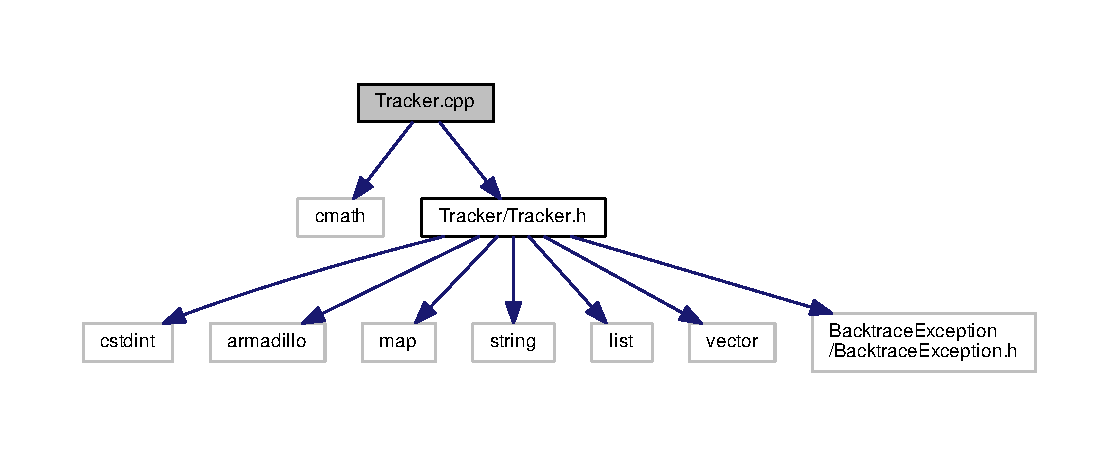
\includegraphics[width=350pt]{Tracker_8cpp__incl}
\end{center}
\end{figure}
\subsubsection*{Namespaces}
\begin{DoxyCompactItemize}
\item 
 \hyperlink{namespacetracker}{tracker}
\end{DoxyCompactItemize}


\subsubsection{Detailed Description}
The member definitions for Tracker. 

\begin{DoxyAuthor}{Author}
Mark J. Olah (mjo at cs.\+unm.\+edu) 
\end{DoxyAuthor}
\begin{DoxyDate}{Date}
04-\/2015 
\end{DoxyDate}

\hypertarget{Tracker_8h}{}\subsection{Tracker.\+h File Reference}
\label{Tracker_8h}\index{Tracker.\+h@{Tracker.\+h}}


The class declaration and inline and templated functions for Tracker.  


{\ttfamily \#include $<$cstdint$>$}\\*
{\ttfamily \#include $<$armadillo$>$}\\*
{\ttfamily \#include $<$map$>$}\\*
{\ttfamily \#include $<$string$>$}\\*
{\ttfamily \#include $<$list$>$}\\*
{\ttfamily \#include $<$vector$>$}\\*
{\ttfamily \#include \char`\"{}Backtrace\+Exception/\+Backtrace\+Exception.\+h\char`\"{}}\\*
Include dependency graph for Tracker.\+h\+:\nopagebreak
\begin{figure}[H]
\begin{center}
\leavevmode
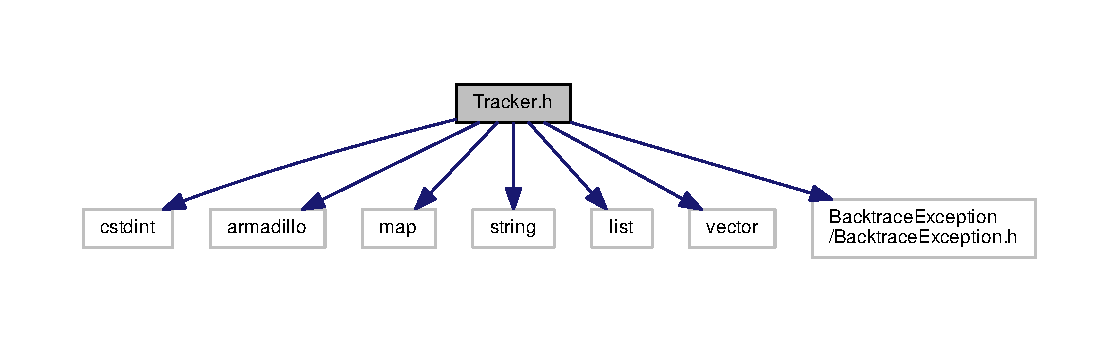
\includegraphics[width=350pt]{Tracker_8h__incl}
\end{center}
\end{figure}
This graph shows which files directly or indirectly include this file\+:\nopagebreak
\begin{figure}[H]
\begin{center}
\leavevmode
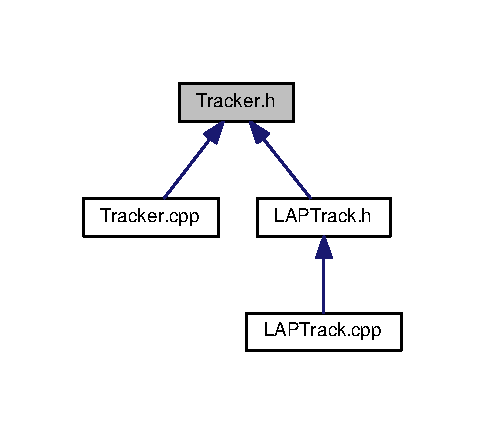
\includegraphics[width=233pt]{Tracker_8h__dep__incl}
\end{center}
\end{figure}
\subsubsection*{Classes}
\begin{DoxyCompactItemize}
\item 
struct \hyperlink{structtracker_1_1ParameterValueError}{tracker\+::\+Parameter\+Value\+Error}
\begin{DoxyCompactList}\small\item\em Parameter value is not valid. \end{DoxyCompactList}\item 
struct \hyperlink{structtracker_1_1LogicalError}{tracker\+::\+Logical\+Error}
\begin{DoxyCompactList}\small\item\em Parameter value is not valid. \end{DoxyCompactList}\item 
class \hyperlink{classtracker_1_1Tracker}{tracker\+::\+Tracker}
\end{DoxyCompactItemize}
\subsubsection*{Namespaces}
\begin{DoxyCompactItemize}
\item 
 \hyperlink{namespacetracker}{tracker}
\end{DoxyCompactItemize}
\subsubsection*{Typedefs}
\begin{DoxyCompactItemize}
\item 
using \hyperlink{namespacetracker_afa61236fc365dda12f9244e9277ddf30}{tracker\+::\+Tracker\+Error} = backtrace\+\_\+exception\+::\+Backtrace\+Exception
\end{DoxyCompactItemize}


\subsubsection{Detailed Description}
The class declaration and inline and templated functions for Tracker. 

\begin{DoxyAuthor}{Author}
Mark J. Olah (mjo@cs.\+unm.\+edu) 
\end{DoxyAuthor}
\begin{DoxyDate}{Date}
2015-\/2019 The base class for all Tracking models
\end{DoxyDate}
Insted of templating on the FloatT type, which is problematic for inheritance hierarchies of templated base classes. Instead wuse a typedef to allow configuration of use with either float/double. Default is double. 
%--- End generated contents ---

% Index
\newpage
\phantomsection
\clearemptydoublepage
\addcontentsline{toc}{section}{Index}
\printindex

\end{document}
